\documentclass[12pt]{report}
\usepackage[utf8]{inputenc}
\usepackage{mathtools}
\usepackage{graphics}
\usepackage[T1]{tgtermes}
\usepackage{subfigure}
\usepackage{float}
\usepackage[left=1.5in, right=1in, top=1in, bottom=1in]{geometry}
\usepackage{nomencl}
\usepackage[hidelinks]{hyperref}
\hypersetup{
    pdftitle={Component 3 Report - Thomas Ward}
}
\usepackage{fancyhdr, lastpage}
\pagestyle{fancy}
\lhead{\textit{Component 3 Report}}

\rhead{\textit{Thomas Ward - Candidate Number 7278}}
\usepackage[Conny]{fncychap}
\usepackage{fancyvrb}
\usepackage{etoolbox}
\usepackage{tikz} 
\usepackage{graphicx}
\usepackage[export]{adjustbox}
\usepackage{soul}

\makenomenclature

\title{Component 3 Report}
\author{Thomas Ward}
\date{September 2020}
\begin{document}

\begin{titlepage} % Suppresses headers and footers on the title page
	\centering % Centre all text
	{\Huge \textbf{Component 3 Report}}\\[\baselineskip] % Title
	{\Large \textbf{Development of an Educational Application}}\\ % Subtitle or further description
	\vfill % Whitespace between the title and the author name
	{\Large Thomas Ward\\ Candidate Number 7278}\\
	\vfill
	{\large 4th October 2021 - 29th Aprill 2022}% Author name
	\vfill % Whitespace between the author name and the rainford text
	Rainford $6^{th}$ Form
\end{titlepage}

\pagebreak

\pagenumbering{roman}
\setcounter{page}{2}

\setcounter{secnumdepth}{0}

\thispagestyle{plain}

\chapter*{Copyright}
\vfill
\begin{center}
© 2022\\
Thomas Ward\\
ALL RIGHTS RESERVED
\end{center}
\vfill

\chapter*{Abstract}
\begin{center}
Thomas Ward: Development of an Educational Application\\
A-Level Computer Science 2020-2022\\
\end{center}

Over the course of this report, I will be identifying the problem I am faced with, which is to create an educational game for high-school students, and also be conducting research into the appropriate field of computer games i.e. platforming games. I will then be developing an educational application for said users.\\

The specific problem I will be facing is that currently, there are no educational applications in which educate the user about the background processes that run when browsing the internet. I aim to produce an application in which fills this gap in education.\\

Previous research suggests that users are more likely to engage with education through the media of playable games. I will be using this knowledge heuristically moving forward with my project.\\

I have found that a two-dimensional navigation game will be most beneficial for this specific instance, as unnecessary details can be easily abstracted. I have then applied this knowledge over the course of my solution, allowing me to create a functional educational application for high-school students.


\chapter*{Dedication}
\textit{This paper is dedicated to David Williams. You have always supported me over the course of my studies and have motivated when I needed it the most.   }

\vfill

\textit{Thank you Dave.}

\vfill

\pagebreak

\chapter*{Acknowledgements}
\begin{center}
I would like to thank Mr D Williams for the motivation to complete this report in the assigned time-frame and to the best of my ability. I would also like to thank the computer science department at Rainford 6$th$ from for their ongoing support across my A-Level journey. My special thanks are extended to the staff of Rainford 6$th$ Form for the overall support provided over the course of studying Computer Science at A-Level.
\end{center}

\vfill
\pagebreak

\setcounter{tocdepth}{3}
\tableofcontents

\addtocontents{toc}{~\hfill\textbf{Page}\par}

\pagebreak

\addcontentsline{toc}{section}{\listfigurename}
\listoffigures

\addtocontents{lof}{~\hfill\textbf{Page}\par}

\pagebreak

\addcontentsline{toc}{section}{\listtablename}
\listoftables

\addtocontents{lot}{~\hfill\textbf{Page}\par}

\pagebreak

\nomenclature{\textbf{JSP}}{Jackson Structured Programming}
\nomenclature{\textbf{PSHE}}{Personal Social Health and Economic}
\nomenclature{\textbf{CPU}}{Central Processing Unit}
\nomenclature{\textbf{FDE}}{Fetch Decode Execute}
\nomenclature{\textbf{NPC}}{Non-Player Character}
\nomenclature{\textbf{OS}}{Operating System}
\nomenclature{\textbf{RAM}}{Random Access Memory}
\nomenclature{\textbf{CSV}}{Comma Separated Values}
\nomenclature{\textbf{IDE}}{Integrated Development Environment}
\nomenclature{\textbf{IDLE}}{Integrated Development Learning Environment}
\nomenclature{\textbf{UML}}{Unified Modeling Language}
\nomenclature{\textbf{STR}}{String}
\nomenclature{\textbf{INT}}{Integer}
\nomenclature{\textbf{BOOL}}{Boolean}
\nomenclature{\textbf{IMG}}{Image}
\nomenclature{\textbf{SDLC}}{Software Development Life Cycle}
\nomenclature{\textbf{FPS}}{Frames Per Second}
\nomenclature{\textbf{EXE}}{Executable}

\printnomenclature
\addcontentsline{toc}{section}{Nomenclature}
\apptocmd{\thebibliography}{\csname phantomsection\endcsname\addcontentsline{toc}{chapter}{\bibname}}{}{}

\pagebreak

\cfoot{Page \thepage\ of \pageref{mylastpage}}


\pagenumbering{arabic}

\setcounter{secnumdepth}{3}

\chapter{Introduction and Computation}

\section{Introduction}
For the component three part of my Computer Science A-level, I will be creating an educational game for the lower years in the high school area of my college. I will be creating the game along with this document to show you my journey through the process of game development and to make any additional comments. In section 1 I will be proposing my idea for my project, talking about who my stakeholder is and the relationship I will have with them and finally talking about the computational methods that I will be implementing into my project and how they will improve aspects of the game.

\section{About Me}
I am a Computer Science driven student studying A-Level Computer Science along with Information Technology and Business Studies at Rainford High. I am keen to expand my knowledge of the engineering side of Computer Science so I will be exploring, experimenting and pushing myself throughout this project to develop my programming skills and report writing at the same time. I will be using Python as my main language in this project as it is the language that I am most familiar with and has some very powerful libraries when it comes to two-dimensional game development. I am also familiar with C++ and may write some sections of code in this language to break it down to a lower level, then analyse the code to further my understanding towards my project. 

\pagebreak

\section{Proposal}
I will be creating a two-dimensional maze-navigating game which aims to educate high-school students about the background processes that go on whilst searching the internet.The game will be called ‘Background’ and will have a minimalist art style. I will also have a stakeholder that I will regularly communicate with and make sure the game meets their expectations and satisfies them. I will be creating all of the art in my game which will allow me to develop my artistic skills as well as software engineering and report writing skills. I will be creating this game to meet my stakeholder’s requirements, adjusting, testing and then consulting with my stakeholder to make sure everything meets their requirements. I will also be creating some in-game music with the help of a friend to pull my game together into a finished product that the user will want to play and learn. The platformer will have multiple levels which vary in detail. There should also be educational screens which aim to educate the students. The game will include a grid-like level system in which the player can navigate. The level will have collide-able walls, collectable items, enemies to avoid, and a door to the next level. The game will also have pop-ups in which a question has to be answered. The question will be based off of a resource pack provided. The students should learn the content and then play the game to retain this information through being quizzed. The fun incentive of the game will encourage students to engage with the curriculum. 

\section{Stakeholder}
My stakeholder will be the head of PSHE. This will enable the head of PSHE to distribute my game to high-school years 7-11. We have had some initial discussions and she has given me some key points to start basing my game off of to get the ball rolling. My stakeholder will use this cyber security game to educate years seven to eleven in my high school and to warn them of the danger of browsing online. Some of the initial ideas that my stakeholder has put forward to me are to make the game user friendly and accessible, for the game to have a simplistic 8-bit art style and for the game to work on the school computers so that it can be used in lessons or of a form time as a PSHE exercise for students. 
\newline
\newline
This solution will benefit my stakeholder as they will be able to use this application within their PSHE curriculum to educate the students. This application will provide a fun and interactive way to convey a segment of the PSHE curriculum in the morning during form time. The stakeholder will require an engaging solution as the users who will be playing will need a high level of engagement to enforce the educational aspect. The stakeholder will need this form of game solution over a  question answer game for this reason.

\pagebreak

\section{Computational Methods}
Computational methods are ways in which problems can be solved by using the computing (computational) power of a computer. Some of these methods are abstraction, backtracking, data mining, performance modelling, pipelining, visualisation and heuristics. All of these computations may not apply to my project so I will just be talking about the relevant methods. 

\subsection{Abstraction}
Abstraction is the process of filtering out unnecessary detail and concentrating on the key details. The process of abstraction is used to break something down to its key constructs and to significantly reduce the complexity of the item. For example, in my project, I will be using abstraction to break down parts of my code and trying to make them as efficient as possible without removing any functionality. I will also be using abstraction in my work to give the art style an ‘8-bit’ appearance which will mean there are minute details that will be removed; however, the style will still be close enough so that you still know which objects are which.

\subsection{Backtracking}
Backtracking is a general algorithm for solving most computational problems. It involves creating a solution by trying an approach and if that approach is unsuccessful, the algorithm will try a different approach and repeat unsuccessful. A backtracking approach does not include trying a random order of potential solutions; the algorithm will try a list of potential solutions and then work backwards if none of the initial list resolve the issue. A perfect example of this is a post-order traversal of a binary tree data structure. The post order traversal aims to list all of the data in each node in ascending order. The search will start by moving down the left-hand side of the tree, constantly looking if there is a node to the right. When a node is found, the traversal backtracks up the tree and continues until the traversal is completed. This usage of backtracking allows certain problems to be solved where a form of trial and error needs to be implemented. I will be implementing a sense of backtracking into the way I develop my project by using this computational way of thinking to debug my code for any errors by working my way through the source code. I will also be taking backtracking into account if my stakeholder wants to change an aspect of the project and I will have to work backwards to append the project suitably.

\pagebreak

\subsection{Heuristics}
A heuristic approach is an approach which considers information that is already known and an approach in which cuts corners based off of this information. For example, when you are crossing the road you would not calculate the velocity of the car coming towards you. You would take a brief glance and make an informed decision on whether it is safe to cross the road or not. I will be using heuristics in my project to make developing the program more efficient and also for implementing certain features such as the educational details about cyber security as this information is known.

\subsection{Performance Modelling}
Performance Modelling is when you see how your software performs on a large scale. You can predict how well the software will run when used on lots of machines at the same time under load. I will be using performance modelling in my project to see how the online scoreboard element of the game will handle 50 requests, 100 requests to even 500+ requests for worst case scenarios. 

\subsection{Pipelining}
Pipelining is the concept of executing instructions to give the appearance of multiple instructions being executed at the same time. Pipelining uses each core of the CPU to perform specific tasks in the FDE cycle in a production line manner. I will be using pipelining in my project to make the game run more efficiently. For example, the game music will be playing whilst the user can play the game. This allows it to look as if the two processes are being processed at once using pipelining. There is a diagram of how pipelining works below.

\begin{figure}[H]
    \centering
    \includegraphics[width=3.5in, frame]{pipelining.png}
    \caption{Pipelining \cite{pipelining}}
    \label{Pipelining}
\end{figure}

\subsection{Visualisation}
Visualization is the process of solving a problem by viewing said problem differently. This approach can be extremely useful when trying to figure out a logical issue in your code. For example, if you are trying to develop a login system then sometimes it is best to work out the logic behind the problem by making a flowchart or writing the problem out in pseudo code. These are all examples of a visual approach to problem solving. 

\subsection{Other Computational Methods}

\begin{itemize}
    \item \textbf{Thinking Abstractly}
    \setlength{\itemindent}{0.3in}
    \item[\textbf{-}] The process of separating specific details from the problem so that a simplified version of the solution is produced.
    \item[\textbf{-}] This will be applied by abstracting level design to remove unnecessary detail, also applying this to any designs e.g., characters.
    \setlength{\itemindent}{0in}
    \item \textbf{Thinking Ahead}
    \setlength{\itemindent}{0.3in}
    \item[\textbf{-}]The process of planning the outcome of a project/piece of code so that the outcome is the one desired and is the same as originally planned.
    \item[\textbf{-}] This will be applied by planning my overall solution and sticking to criteria that I will predefined before starting development.
    \setlength{\itemindent}{0in}
    \item \textbf{Thinking Procedurally}
    \setlength{\itemindent}{0.3in}
    \item[\textbf{-}] This  is  the  process  of  breaking  down  large  tasks  into smaller sub-tasks so that they become easier to solve/complete.
    \item[\textbf{-}]This will be applied by separating elements of my code into functions to  allow  for  maintainability  of  my  code.   Also,  by  breaking  down  large  tasks  into sub-tasks to make the project more manageable. 
    \setlength{\itemindent}{0in}
    \item \textbf{Thinking Concurrently}
    \setlength{\itemindent}{0.3in}
    \item[\textbf{-}] The process of executing more than one task at a time.This speeds up processing time and allows for a more polished looking solution.
    \item[\textbf{-}] This will be applied by having multiple processes seem to be completed simultaneously e.g., music and game running at the same time.
    \setlength{\itemindent}{0in}
    \item \textbf{Thinking Logically}
    \setlength{\itemindent}{0.3in}
    \item[\textbf{-}] The process of applying rules to problem solving. Algorithms designed as a set of steps to follow to solve a problem. 
    \item[\textbf{-}] By creating flow chart diagrams to map out the flow of my program.
    \setlength{\itemindent}{0in}
\end{itemize}

\pagebreak

\chapter{Research and Requirements}
\section{Field Research}
I will begin my project by researching similar games in which certain features may overlap. I will be finding games with similar elements that I would like to implement into my game, analysing these features in depth and then explaining how I will use and implement these into my project. 

\subsection{High Strangeness}
High Strangeness is a top-down adventure game in which the user switches between a sixteen- and eight-bit art style. The player uses generational differences in the art styles. High Strangeness uses the same camera angle in which I will use in my game. It is a top-down view where the camera follows the room or square the player is in. This is a static game camera in which I will be aiming to implement in my game. The art style of High Strangeness is also similar to the one I will be aiming to use within my project so that it looks professional and clean. The game switches between the eight-bit art style and the sixteen-bit art style flawlessly, giving the user an excellent experience whilst playing the game. High Strangeness is also similar to my idea as you can explore a map looking for objects to interact with and people to talk to. The game is also not very machine intensive so this would benefit me as my game will need to run on school computers with a low specification. \cite{high strangeness}  

\begin{figure}[h]
    \centering
    \includegraphics[width=5in]{highStrangeness.jpg}
    \caption{High Strangeness \cite{high strangeness}}
    \label{HighStangeness}
\end{figure}

\pagebreak

\subsection{Hyper Light Drifter}
Hyper Light Drifter is a top-down adventure game in which the player explores an open world through a thirty two-bit art style. The combat in this game is excellent so I will be using this game as a target when I implement the combat elements of my game. In Hyper Light Drifter, you can also navigate the world and interact with enemies, objects and NPC’s. I have included a screen shot from the game whilst the player is in combat \cite{hyperL}. 

\begin{figure}[H]
    \centering
    \subfigure[Fig.a]{
    \includegraphics[width=2.75in]{HLD1.jpg}
    }
    \subfigure[Fig.b]{
    \includegraphics[width=2.75in]{HLD2.jpg}
    }
    \caption{Hyper Light Drifter \cite{hyperL}}
\end{figure}

\pagebreak

\subsection{LEGO Harry Potter Years 1-4}
The Lego Harry Potter games use an open world map extremely well. The game also includes gold coin collectables which I will have in my game. The game allows the user to collect these coins and keeps track of the number of coins each user has. I will be implementing this feature into my game as a score counter. Each user’s score will then be displayed onto a leader board for everyone to view. The user will accumulate scores by completing educational tasks about cyber security \cite{harryP}. 

\begin{figure}[h]
     \centering
    \subfigure[Fig.a]{
    \includegraphics[width=4in, frame]{harryp1.jpg}
    }
    \subfigure[Fig.b]{
    \includegraphics[width=4in, frame]{harryp2.png}
    }
    \caption{Lego Harry Potter Years 1-4 \cite{harryP}}
\end{figure}

\subsection{Pokemon Crystal}
Pokémon Crystal is one of the first Pokémon games to be released for the Gameboy Colour. Pokémon has an excellent screen layout for when you are interacting with an NPC or battling another Pokémon trainer. I will be implementing a similar interaction screen in my game which will be based off of the one in Pokémon Crystal. The text boxes are very well placed, and I will be using a similar layout as well as the button layout to be able to interact with the NPC’s \cite{pokemonC}.

\begin{figure}[H]
     \centering
    \subfigure[Fig.a]{
    \includegraphics[width=4.5in, frame]{pokemon1.png}
    }
    \subfigure[Fig.b]{
    \includegraphics[width=4.5in, frame]{pokemon2.png}
    }
    \caption{Pokemon Crystal \cite{pokemonC}}
\end{figure}

\pagebreak

\subsection{Pokemon X and Y}
Pokémon X and Y was developed for the Nintendo    
3DS and is the 15Th game in the franchise. This Pokémon game features an incredible map which is displayed on the top screen on the console as the player navigates the open map. I will be implementing a similar feature to my game with the map in the top left of the user’s screen. There will be a marker that constantly updates on the map to mark the players location at all times to allow them to navigate the map which is inside of a high school \cite{pokemonXY}.

\begin{figure}[h]
    \centering
    \includegraphics[width=\linewidth, frame]{pokemonXY.png}
    \caption{Pokemon X and Y \cite{pokemonXY}}
    \label{PokemonXnY}
\end{figure}

\clearpage

\section{Viability Research}
I have conducted some further research into whether there is a need for my project. I have conducted a google survey to dive deeper into the users of my solution and find out what they think about the viability of my solution. 

\subsection{Viability Evidence}
The two-dimensional platformer that I will be creating will be a popular game amongst my target audience. I know this because platforms are one of the most popular genres of video games, second to puzzle games. There is a graph below to support this \cite{viabilityG}.

\begin{figure}[ht]
    \centering
    \includegraphics[width=\linewidth, frame]{viability.png}
    \caption{Solution Viability Graph \cite{viabilityG}}
    \label{SolutionViabilty}
\end{figure}

\section{Summary of Research}
The research that I have collated about various open world games has given me an excellent idea into how to implement character interactions into my game. As I will be creating a two-dimensional platformer, I mainly conducted my research around interacting with NPC’s as this is the part of the game where extra external knowledge was required. This research has given me many more ideas of how I will implement this mechanic into my game.

\pagebreak

\section{Stakeholder Conversation}
After proposing my solution and summarising my research, I have presented this to my stakeholder. Overall they are pleased with the eligibility of my solution. Going forward me and my stakeholder have decided to devise a set of limitations and a success criteria. The stakeholder has asked for this research to be conducted as they want to be made aware of any potential problems/limitations that may be presented in the future. They have also asked for a success criteria to be generated so that it can be referred back to into the future. The success criteria should contain the key areas of my solution and then sub-points explaining in further detail the point above. Here is an email from my stakeholder explaining how they would like to see this presented.

\begin{figure}[ht]
    \centering
    \includegraphics[width=\linewidth, frame]{stakeholder1.png}
    \caption{1st Stakeholder Conversation}
    \label{stakeholder1}
\end{figure}

\pagebreak

\section{Meeting Notes}
Whilst in the meeting with my stakeholder, I made some notes about the meeting. These notes contain information about the aim of the meeting and also what was achieved in the meeting. I will display these notes below.

\begin{figure}[H]
    \centering
    \includegraphics[width=\linewidth, frame]{meetingnotes1.PNG}
    \caption{Meeting Notes}
    \label{stakeholder1}
\end{figure}

\pagebreak

\section{Limitations}
In my project I am going to find some drawbacks and limitations to stop me from doing exactly what I would like to during development. I will be discussing these limitations below and explaining what steps I can take to work around these limitations. 

\subsection{Software Limitations}
I will be programming my game in Python using a game function library called Pygame. Python is very good for the basic game development features that I need for my game, however these features limit the complexity of the project. To program a game is immensely complex and using Python will make the process easier whilst still delivering an amazing level of game opportunities. The logic in the game will be minimalist as this is all the Pygame library allows for. 

\subsection{Programming Limitations}
As powerful as the Pygame library is, my programming skill will limit the complexity of the game. I have only been programming in python for 3 years so I am considered a beginner and I will be constantly learning throughout this project. I will also be writing in python which only has limited debug features so I will have to look through my code and plan out how to fix any logical errors.

\subsection{Hardware Limitations}
The computers that I am designing this game for are only schoolwork stations with low specifications. This means that the program that I create will have to be very easy to run as the computer’s hardware will limit the performance of the game. This means I will also have to spend extra time optimising my code to make it run as efficiently as possible on these machines. 

\subsection{Time Limitations}
This project needs to be completed before March of 2022, so specific time deadlines must be met to make sure the game has had maximum development in the time frame given to me. This means I will only be able to spend a limited amount of time on coding the logic and designing the artwork which means the project will be limited to as much as I can do a week. This will keep the project small and with no over-ambitious goals that will not be completed at the end of the time frame. 

\pagebreak

\subsection{Stakeholder Limitations}
My stakeholder will have a large impact on the outcome of my project as I am making it to their specifications and design ideas as the game is ultimately for them to distribute. They will tell me if they do not like a feature and I will have to make updates and edit said feature to meet the requirements they have set for me. This may not always be the best idea in terms of development for the project, but I will have to abide by their command and append the project accordingly. 

\subsection{Creative Limitations}
The creative limitations of this project will limit the success of the outcome. For example, I am not the greatest graphical designer so the artwork will be basic and to my ability. Additionally, I may not be able to think of new, innovative ideas for my project so there will be some ideas that are commonly seen in similar games to add functionality to the game. I will also be limited by thinking of logical solutions to some of my problems as they might be too complex to solve.

\subsection{Learning Theory Limitations}
There will be a limit to how effective the educational aspect of my application will be. This is because I have no training/qualifications in teaching, and no prior first-hand research/knowledge when it comes to educating. The solution I will generate is what I think will be the most effective for my stakeholders users based on heuristic knowledge. My lack of teaching knowledge could also mean that this 'gameified' solution isn't the best way to educate the students, but I think it will be at least engaging as these students will enjoy the game aspect.   

\section{Hardware and Software Requirements}
My game will be developed in the Godot game engine which has relatively easy to run hardware requirements. The game engine uses the OpenGL game development code library. I will list the specific hardware requirements for a Windows machine and a Macintosh below. The school I am building this game for has Windows and Macintosh machines. 

\small
\paragraph{Requirements}
\begin{itemize}
    \item {Modern Operating System}
    \setlength{\itemindent}{0.5in}
    \item \textit{Windows 7 or 10}
    \item \textit{Mac OS X 10.11 or higher; 64-bit}
    \item \textit{64-bit CPU (Intel / AMD architecture)}
    \setlength{\itemindent}{0in}
    \item 4GB of RAM
    \item 5GB of free disk space
\end{itemize}
\normalsize

\pagebreak

\section{Overall Project Success Criteria}
My project requires a list of features so that progress can be achieved and goals can be completed. These elements of my project must be completed to make it a success. I have spoken to my stakeholder and agreed on these success criteria. My game must:

\footnotesize
\begin{enumerate}
    \item \textbf{Always include a fully functioning exit game button}
    \item \textbf{Include a scoreboard with all of the players scores displayed on it}
    \setlength{\itemindent}{0.5in}
    \item[a.]Scores stored in external file
    \item[b.]Scoreboard data read from external file
    \item[c.]Program writes the users score and username to the scoreboard file
    \item[d.]Data for each user stored on a new line
    \setlength{\itemindent}{0in}
    \item \textbf{Include a multi room game}
    \setlength{\itemindent}{0.5in}
    \item[a.] Levels must all be the same size
    \item[b.] Levels must be stored in external data files
    \item[c.] Levels must be ascending in difficulty order
    \setlength{\itemindent}{0in}
    \item \textbf{Include characters that the player can interact with}
    \item \textbf{Include objects that the player can interact with}
    \setlength{\itemindent}{0.5in}
    \item[a.] Coins which add a score point
    \item[b.] Enemies which reset the player
    \item[c.] Exit gates which lead to the next level
    \setlength{\itemindent}{0in}
    \item \textbf{Work on all computer systems within the school}
    \setlength{\itemindent}{0.5in}
    \item[a.] This means it must be optimised for these computers as these machines do not have much processing power
    \setlength{\itemindent}{0in}
    \item \textbf{Convey information in an educational and easy to understand manor}
    \setlength{\itemindent}{0.5in}
    \item[a.] This can be done through simple question screens
    \item[b.] Answers should be key terms/words to maximise ease of answering each question
    \setlength{\itemindent}{0in}
    \item \textbf{Working character animations}
    \item \textbf{Working physics for player characters}
    \setlength{\itemindent}{0.5in}
    \item[a.] Players must stop when collided with wall
    \item[b.] Player must reset when collided with an enemy
    \item[c.] Score incremented when player interacts with coin
    \item[d.] Player can move up, down, left and right around the game window.
    \setlength{\itemindent}{0in}
    \item \textbf{Working score counter visible to the player when playing the game}
\end{enumerate}
\normalsize

\pagebreak

\section{Further Stakeholder Discussion}
I have liaised with my stakeholder after presenting them with these requirements and limitations. I have also presented them with the success criteria that I have generated based on their previous feedback. Overall my stakeholder was pleased with the reasonable set of limitations and success criteria that I had produced for them. My stakeholder has now asked me to produce some designs. They would like me to do most of the playing on this stage also. They have asked me to present them with elements of the list presented below in our email communications.

\begin{figure}[h]
    \centering
    \includegraphics[width=6in, frame]{stakeholder2.png}
    \caption{Further Conversation with Stakeholder}
    \label{stakeholder2}
\end{figure}

\pagebreak

\section{Further Meeting notes}
Whilst in the meeting with my stakeholder, I made some notes about the meeting. I will display these notes below.

\begin{figure}[H]
    \centering
    \includegraphics[width=5in, frame]{meetingnotes2.PNG}
    \caption{Meeting Notes}
    \label{stakeholder2}
\end{figure}

\pagebreak

\chapter{Design and Testing}

\section{Menu Designs}
I have created a hand drawn menu design. This design will be a baseline for me to create computer-generated designs off of. The menu design that I have drawn is an abstracted version of the designs that will be used in my actual game. This has allowed me to generate basic ideas which can be developed at a later point.

\begin{figure}[H]
    \centering
    \subfigure[Fig.a]{
    \includegraphics[width=2.75in, frame]{hand drawn 1.jpg}
    }
    \subfigure[Fig.b]{
    \includegraphics[width=2.75in, frame]{hand drawn 2.jpg}
    }
    \caption{Hand Drawn Menu Designs}
\end{figure}

I have created a minimalist main menu and retry screen. I have designed the screens this way as it fits into the abstracted theme of my game. On the menu screen, there is the games logo, a play button, a quit button and a mute sounds button. This allows the user to mute the in-game sounds if they need to. The play button takes the user to the first level in the game. The quit button properly exits the program if the user would like to. These are the necessities of a main game menu and will remain the same throughout the development process of this game. The retry screen also fits into the abstracted theme of my game. The retry screen displays the final score of the player in the top left corner of the screen. This is so the player knows what they scored that round. There is also a button to play again, as well as a quit game button for players who wish to quit.

\section{Level Designs}
I have created an abstracted hand drawn level design which will then help me create these levels in more detail digitally later on. These designs will be of the starting level, and an example of an NPC interaction.

\begin{figure}[H]
    \centering
    \subfigure[Fig.a]{
    \includegraphics[width=3in, frame]{hand drawn 3.jpg}
    }
    \subfigure[Fig.b]{
    \includegraphics[width=3in, frame]{hand drawn 4.jpg}
    }
    \caption{Hand Drawn Level Designs}
\end{figure}

\pagebreak

Above, I have created an example of a level design combining multiple game elements and also an example of the player's interaction with an NPC. In the NPC interaction example, I have drawn what I want an educational interaction to look like. The NPC should give the user a fact about security on the internet and also prompt the user to write it down. These facts will then be used to test the students after they have played the game. This will help cement this knowledge into the students memory. The level that I have designed will be the first level in my game. It teaches the basic mechanics (jumping and avoiding lava) whilst still being fun. The level is made up of tiles which can represent a number of different blocks. There are grass, dirt, lava, platform and a door block which all interact differently with the player. 

\section{Design Feedback}
After completing these designs, I presented them to my stakeholder. My stakeholder's general consensus was to make the levels more complicated. This is in relation to the size and amount of obstacles per level. This can be easily achieved as when I am developing the levels, I will increase the size of the grid. This will allow more obstacles per level. The other change they suggested was to add a knowledge test after the game has been completed. This is to cement the information that is presented thought the game. I have inserted a screenshot of the email from my stakeholder explaining this. 

\begin{figure}[H]
    \centering
    \includegraphics[width=6in, frame]{stakeholder3.png}
    \caption{Stakeholder Design Improvements}
    \label{stakeholder3}
\end{figure}

\clearpage

\section{Design Amendments}
Following the feedback given to me by my stakeholder above, I have made some amendments to the designs level design. I have made the grid 20x20 instead of the 8x10 used in the hand drawn design. I have also made this design on the computer to get one step closer to final game.

\paragraph{Level Design}
Below, I have created a mock-design of what I would like the final solutions' levels to look like. This example level includes the player, collectable coins, an enemy, and an exit gate to the next level. 

\begin{figure}[H]
    \centering
    \includegraphics[width=5in,frame]{Leveldesign.png}
    \caption{Computer-Generated Level Design}
    \label{leveldesign}
\end{figure}

\clearpage

\section{Gantt Chart}
I have created a gantt chart to plan my time over the course of this project. This gantt chart allows me to keep track of my progress and where I would like to be up to each week. This will also satisfy my stakeholders demands as they have asked for a gantt chart to be produced in our last conversation. I will be using RAD to develop my software. 

\begin{figure}[h]
    \centering
    \includegraphics[width=\linewidth, frame]{gantt chart.png}
    \caption{Gantt Chart}
    \label{gantChart}
\end{figure}

\section{Problem Decomposition Using JSP}
To make my project more manageable, I have decomposed the project into smaller, more manageable sub-sections. This method is called Jackson Structured Programming, or otherwise known as Stepwise Refinement. This will allow me to visualise the problem I am faced with. This is a good example of the computational method Visualization and how it can be applied within a development scenario.

\begin{figure}[h]
    \centering
    \includegraphics[width=6in, frame]{JSP.png}
    \caption{Decomposition Using JSP}
    \label{JSPmodel}
\end{figure}

\pagebreak

\section{Flowcharts}
I have created 5 flowcharts to visualise the flow of my program. Each flowchart symbol represents a different process/decision within my program; some lead to other sub-routines within the program.

\paragraph{Main Program and Menu Screen}
 The first flowchart I have created is the main program. This is just a line of subroutines as most of the computation is performed inside of functions or classes. The second flowchart that I have created is the flow of the menu screen. Each button is loaded onto the screen. The user then has a choice of which button they would like to click. The appropriate action is then taken e.g it loads the appropriate function. 

\paragraph{Login System and Leader-board}
In these flow charts I have visualized the Login System and the leader-board functions in my program. I have tried to represent as closely as possible all the steps that take place when the login system is run. It has an attempt limiter and also checks usernames and passwords compared to a CSV file. This is beneficial as the user can store/delete accounts easily. This login system will be primarily used by admins to access questions and their answers etc. I have also created a flow chart to map out the flow of the function in which lists all the scores in a leader-board manner. This function opens a CSV, prints the values in the first and second columns, and then closes the CSV. Finally it returns back to the menu screen. This effectively gives the user a print out of the top scores and the usernames of the users who had scored said score.

\paragraph{The Main Game}
In this flowchart I have represented the main game loop. The main game loop flowchart is more complex than the others as this is where most of the updating and computation happens. The function starts off by creating a ‘while the game is running’ loop. The function then blits the background, level, and player to the screen. This is how each element of the game is drawn to the screen. This is a highly abstracted model of what will actually happen in my program code. The function then checks to see if the player is alive. If yes, it then checks if the player has moved. If the payer has not moved, the function just repeats. If movement is detected, the function will then calculate the new player position on the screen and also move the player to there. Again, this is a highly abstracted process from the one in which will occur in my program code. The function then checks for any collisions with collectables e.g a coin. If contact with a coin is made, a point will be added to the player's score count. If not, the function performs one final check. It checks to see if the player is in contact with the level exit door. If so, the level counter is incremented by one. If the player makes contact with dangerous blocks such as lava or enemies, the function will detect this and break from the loop, presenting the player with the retry or quit screen.

\pagebreak

\begin{figure}[H]
    \centering
    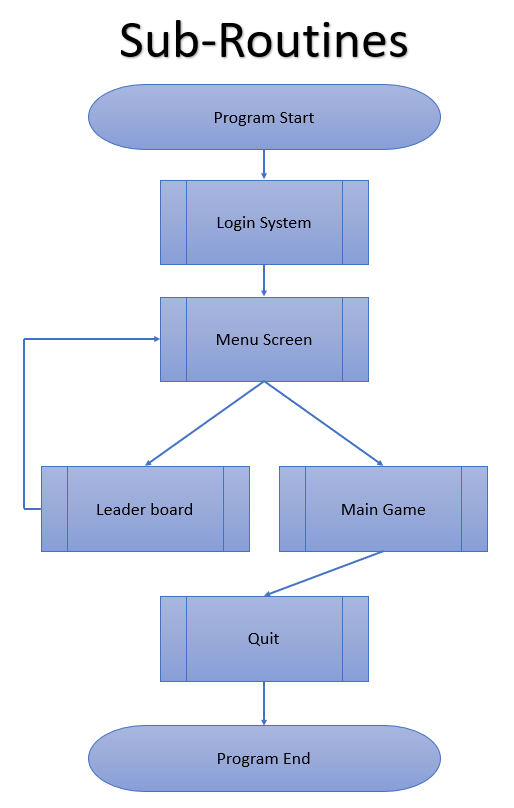
\includegraphics[width=5.4in, frame]{flowchartSubroutines.PNG}
    \caption{Sub-routines Flowchart}
    \label{flowc1}
\end{figure}

\begin{figure}[H]
    \centering
    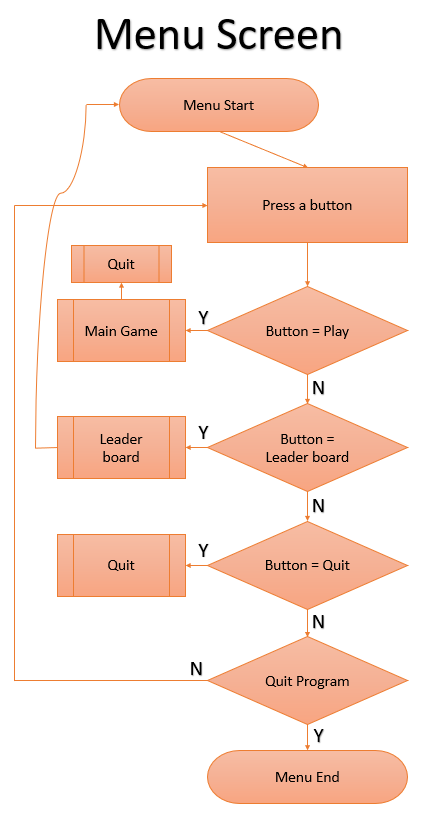
\includegraphics[width=4.5in, frame]{flowchartMenu.PNG}
    \caption{Menu Screen Flowchart}
    \label{flowc2}
\end{figure}

\begin{figure}[H]
    \centering
    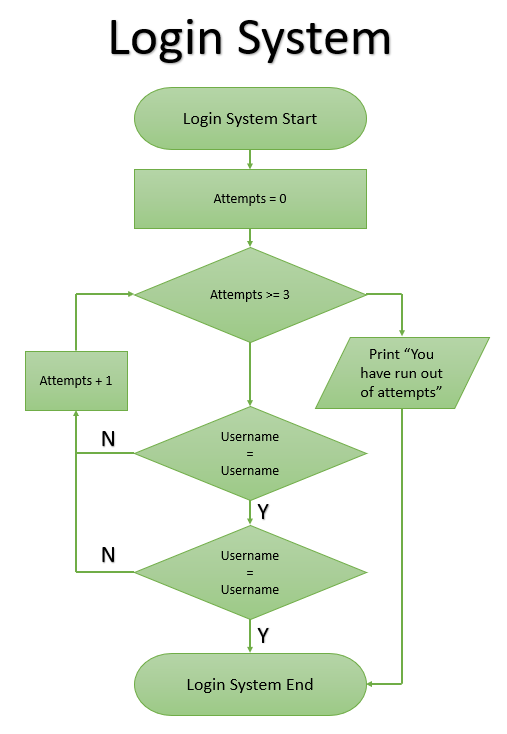
\includegraphics[width=5.75in, frame]{flowchartLogin.PNG}
    \caption{Login System Flowchart}
    \label{flowc3}
\end{figure}

\begin{figure}[H]
    \centering
    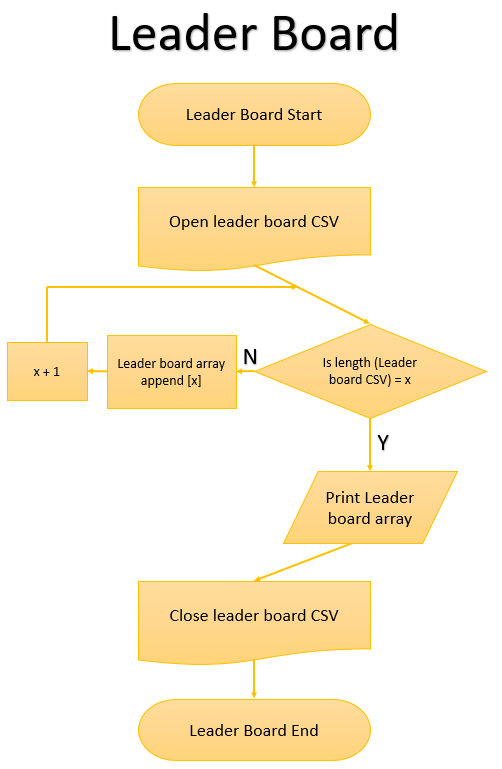
\includegraphics[width=5.5in, frame]{flowchartLeaderboard.PNG}
    \caption{Leader-board System Flowchart}
    \label{flowc4}
\end{figure}

\begin{figure}[H]
    \centering
    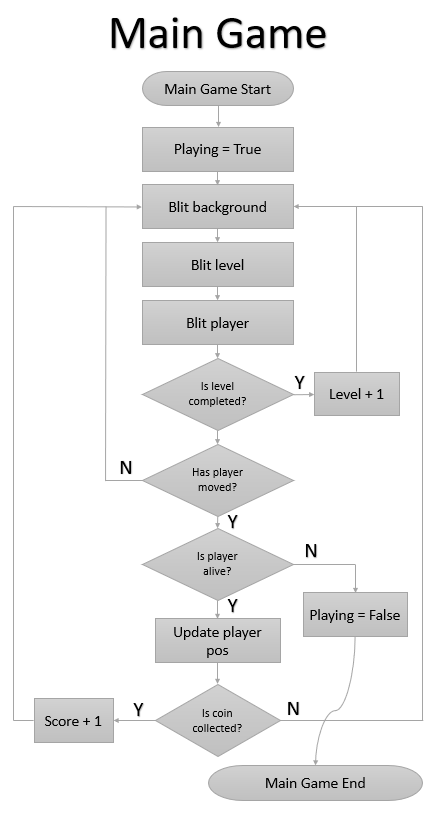
\includegraphics[width=4.5in, frame]{flowchartMain.PNG}
    \caption{Main Game Flowchart}
    \label{flowc6}
\end{figure}

\pagebreak

\section{Pseudo Code}
I have created some pseudo code to give me an idea of what certain parts of the program will look like. The pseudo code gives a simplified view ow what a section of could should look like when being developed.

\begin{Verbatim}[numbers=left, frame=single]
FUNC loginSystem():
    username = INPUT("Enter username: ")
    loggedin = FALSE
    i = 3
    WHILE loggedin == FALSE and i > 0:
        FROM CSV "usernames.csv"
        FOR x in CSV:
            IF username == CSV[x]:
                PRINT("Username correct")
                password = INPUT("Enter password: ")
                FROM CSV "passwords.csv"
                FOR x in CSV:
                    IF password == CSV[x]:
                        PRINT("Password correct")
                        loggedin = TRUE
                    ELSE:
                        PRINT("Password not found")
                        i - 1
            ELSE:
                PRINT("Username not found")
                i - 1
    RETURN username
\end{Verbatim}

\section{Validation}
I will be using validation throughout my program code for multiple reasons. The main reason is to check the users keyboard inputs in which control the player sprite. Validation is used in this application to check the button pressed corresponds to the correct movement i.e when the left arrow is pressed, the player moves left. Validation can also be used to check the answers provided by students in the quiz portion of my program.  

\pagebreak

\section{UML Diagram}
I have created a UML diagram to visualise how the class structure will work in my solution. The Classes that are highlighted are the super classes. This means that they do not inherit any methods or attributes from any other classes. This is a good way to visually represent how each of my classes inherits, if it does at all. Each class has attributes and methods. An attribute is a variable assigned to the instance of the class, and a method is a function inside of a class. There are also private and public attributes. A private attribute can not be modified by any other classes, whereas a public attribute can be changed globally. 

\begin{figure}[h]
    \centering
    \includegraphics[width=6in, frame]{Screenshot 2022-01-31 102128.png}
    \caption{Object-Orientated Programming UML}
    \label{UML}
\end{figure}

\pagebreak

\section{Plans for Iteration Each Iteration}
\paragraph{Iteration 1}
In iteration 1, I will be creating a basic maze-like game. Features will include a basic character movement system with a single basic level. The game should be playable to a basic level with the appropriate collisions in place. The collisions will work by predicting where the player will move, and if they intersect with a level piece, the player will stop. There should also be a working 'x' button so that the user can exit the game at any time. 

\paragraph{Iteration 2}
In iteration 2, the game should be similar to iteration 1 with more levels implemented into the solution. This can be achieved by creating the levels in a text document and importing said text document into python. The levels are constructed by assigning each square of the level a value between 1-10. Each value represents a certain tile i.e dirt, grass or lava etc. 

\paragraph{Iteration 3}
In iteration 3, I would like the final solution to be nearly complete. This means a fully playable platforming game, with multiple levels and a start screen. There should also be collectable coins, moving platforms, moving enemies, and lava to add an element of difficulty to each level. There should also be a working door in each level so that the player can progress to the next level.

\paragraph{Iteration 4}
In iteration 4, my solution should be fully complete with minimal errors. The game should also include informational slides in between levels. This is to educate the users about cookies and background processes when using the internet. There should also be a quiz at the end to test the students on the information that is provided to them throughout the game. There should also be a working scoreboard which displays the name and score, in descending order, of the top 15 students. 


\section{Testing}
I will be testing my game following the SDLC cycle. SDLC stands for systems/software development life cycle. This involves designing the program; Implementing the designed features; testing the features; evaluating said features and then analyzing these newly implemented features. This is a form of iterative testing. As Well as this iterative testing, I will be testing my program at the end of development to check for errors/bugs. This is called final testing. I will also be white box testing my game, which is when the developer checks the code manually for errors. After the game has been white box tested, I will be completing some black box testing also, after highlighting any syntax errors. Black box testing is when the game is tested via playing through each element and testing if it works correctly. I will be presenting these test results in the test table below. 

\pagebreak

\section{Why is Testing Needed?}
Testing is needed throughout the development of this solution for multiple reasons. First and foremost, testing will be used throughout this project to ensure the final solution is working in the specified, intended way. This stops the end-users complaining and returning my solution with negative feedback. A fully working solution also means that the game will have the maximum impact on the students. 

\section{Testing Within Each Iteration}
\paragraph{Iteration 1}
Testing will be used throughout iteration 1 to ensure the fundamentals of the program are working in correct order. I hope to test to see if the images load into the program properly. This will give me a good indication of the scale of each image. I will be able to see if the image's resolution needs to be changed. This will be done by using black box testing. I will be including a test table for each iteration, within each iteration.

\paragraph{Iteration 2}
Over the course of iteration 2, I will be primarily black box testing my game to ensure the fundamentals are working correctly. This will then ensure a solid base game is generated which can be built up throughout iteration 3 and 4. 

\paragraph{Iteration 3}
During my time developing iteration 3,  I will be completing both white and black box testing. This is to insure the code and program flow are working and can be maintained to a high level. I will also preform alpha-testing by handing my game to my peers to test for me. This may highlight some fundamental errors. A second or third perspective can be beneficial as they may have a different sub-conscious way of testing. 

\paragraph{Iteration 4}
In iteration 4, I will have completed a full test table. I will be testing in small amounts to ensure the newly implemented features from the previous iteration. I will also be testing the end of game quiz. This testing will be both white and black box testing. I will be testing if the program can read from a CSV, and then write the players score to a separate CSV file.

\pagebreak

\chapter{Iteration 1}

\begin{figure}[h]
    \centering
    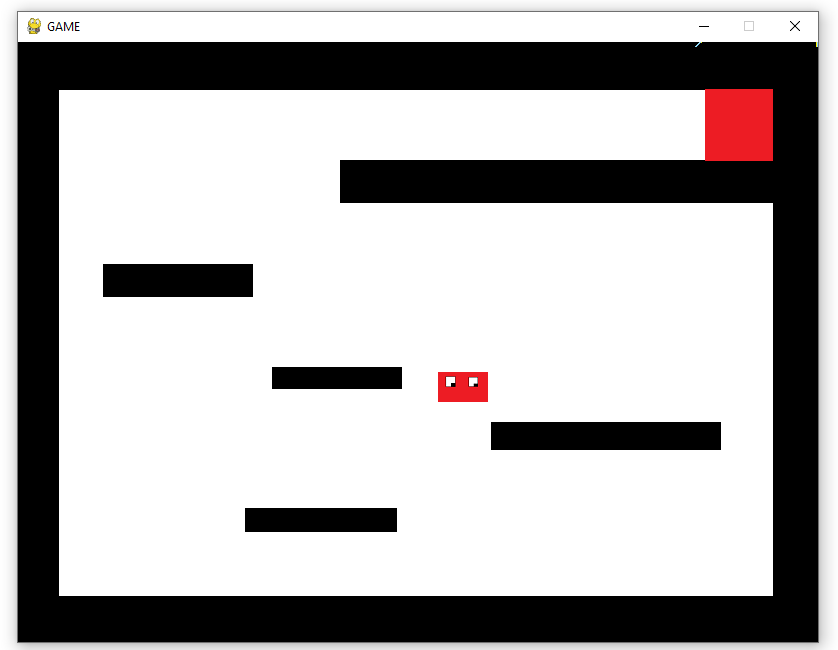
\includegraphics[width=\linewidth]{iteration1title.png}
    \label{iteration1title}
\end{figure}

\pagebreak

\section{Introduction}
Over the course of iteration 1, I will be developing a basic maze game, along with a basic level system. This iteration should achieve a number of aims in which I will set in the success criteria below.

\section{Iteration 1 Success Criteria}
Throughout Iteration 1, I will be developing with the intention of my game being able to:

\begin{enumerate}
    \item run on a school computer at 60 FPS.
    \item run in a separate game window from the python IDLE shell.
    \item display a working player model with basic collisions.
    \item display a background to the game window.
    \item close when the 'X' button is pressed at any time.
    \item all files saved into a single project folder.
    \item include basic platform for development i.e creation of classes, ready for iteration 2.
\end{enumerate}

\paragraph{why?}
I will be referring to this mini success criteria throughout iteration 1, and using it to evaluate the success of each test. I will also be using this success criteria to help guide me code each individual feature of the game. This is a more specific version of the main success criteria, with a few points decomposed. 

\pagebreak

\section{Test Plan for Iteration 1}

\paragraph{What I Plan to Test}
Testing will be used throughout iteration 1 to ensure the fundamentals of the program are working in correct order. I hope to test to see if the images load into the program properly. This will give me a good indication of the scale of each image. I will be able to see if the image's resolution needs to be changed. This will be done by using black box testing. I will be including a test table for each iteration, within each iteration.

\begin{table}[H]
    \centering
    \begin{tabular}{|c|c|c|c|}
    \hline
    \textbf{*} & \textbf{Test Description} & \textbf{Test Data} & \textbf{Expected Outcome}\\
    \hline
    1 & 800 x 600 game window is & Executing code. & Game window opens successfully\\
    & created. & & in python.\\
    \hline
    2 & Background image is & On start-up. & Image is loaded when the\\
      & loaded.              &             & program is run. \\
    \hline
    3 & Background image is & On start up. & The image is displayed onto\\
    & displayed. & & the game window. \\
    \hline
    4 & The 'X' button closes & On press. & The program will close.\\
    & the program. & & \\
    \hline
    5 & A player image is & On start-up. & The program will display the \\
    & displayed to the game & & players sprite to the game \\
    & window. & & window.\\
    \hline
    6 & The player has basic & On left or & The player will move to the\\
    & movement in the $x$ direction. & right button & left or right, depending on \\
    & & press. & the input.\\
    \hline
    7 & The player has basic & On up or down & The player will move up or\\
    & movement in the $y$ direction. & button press. & down, depending on the button\\
    & & & pressed. \\
    \hline
    \end{tabular}
    \caption{Iteration 1 Pre-Development Testing Plan}
    \label{TestTable}
\end{table}

\pagebreak

\section{Code Development}
I will be displaying my program code for iteration 1 below and justifying the rationale behind my decisions when creating this code.

\subsection{Libraries, Initialisation, Globals and Display}
Here I have displayed the first section of my code. I will be breaking down my code into each of its individual elements. I will then be justifying my decisions throughout.

\small

\begin{Verbatim}[numbers=left, frame=single]
### LIBS ###
import pygame   # Imports the pygame library                                   
import time     # Imports the time library                                        

    
### INITIALISATION ###
# Initialises the pygame module
pygame.init()       
# Creates a clock to regulate updates
clock = pygame.time.Clock()        


### GLOBALS ###
# RGB value for red
red = (255,0,0)     
# Height and width of the game window
height, width = 600, 800     
# Assigns the frames per second
fps = 60                                                            


### IMAGES ###
# Loads the player image
player1_img = pygame.image.load("p1.png")
# Loads the background image
backG = pygame.image.load("background.png")


### DISPLAY ###
# Creates a game display with the height and width that is asigned
gameDisplay = pygame.display.set_mode((width, height))
# Sets application caption
pygame.display.set_caption('GAME')                                  
background_rect = pygame.Rect((0,0),(width,height))
\end{Verbatim}

\normalsize

\pagebreak

\subsubsection{Libraries}
Here are the libraries in which I have used so far in my program. The first library, \textit{import pygame}, is used to import the Pygame game library. This library has many features such as the creation of game windows, bliting images to the screen, and many more features. 

The library \textit{import time} is used to import a clock into python. This clock can be used to display the date, set a timer, and can add pauses to the program. 

\begin{Verbatim}[numbers=left, frame=single]
### LIBS ###
import pygame                                                       
import time  
\end{Verbatim}

\subsubsection{Initialisation}
These two lines of code initialise the pygame library, and also create a clock to keep the game at a set FPS. \textit{pygame.init()} calls the constructor class of Pygame. This assigns all the appropriate variables to the attribute \textit{self}.

\textit{pygame.time.clock()} calls the internal clock method within Pygame. This is then used further in the program to tick the clock, and also to regulate the FPS of the game.

\begin{Verbatim}[numbers=left, frame=single]
### INITIALISATION ###
pygame.init()                                                       
clock = pygame.time.Clock()
\end{Verbatim}

\subsubsection{Globals}
Global variables are variables in which can be called at any point in the program. They are in the global scope of the program, not a local scope. This means they can be passes into any function without having to be returned from another. \textit{red} assigns the RGB value \textit{255,0,0} so that it can be referenced at any point later in the code. If this value changes, any times \textit{red} is used, it will change accordingly. 

\textit{height} and \textit{width} are used to set the size of the game window. Having these variables in the global scope allows these values to be changed easily. If the game window needs to be \textit{800,800} for example, one number change in the global scope will change the value throughout the program.

\textit{backG} sets the background image for the game. For now, I have just used a .png of what a level will look like.  \textit{fps} sets the FPS of the game. I have chosen \textit{60} as most monitors are typically \textit{60 Hz}.

\begin{Verbatim}[numbers=left, frame=single]
### GLOBALS ###
red = (255,0,0)
height, width = 600, 800                                
backG = pygame.image.load("background.png")                         
fps = 60 
\end{Verbatim}

\pagebreak

\subsubsection{Images and Display}
\textit{player1\_img} sets the image for player 1. This allows the image code to stay the same, whilst still being able to change the contents of the image. As long as the player image is saved as \textit{p1.png}, the appropriate image will be loaded and displayed within the game.

The display element of the code creates the run time environment for the program to run in. \textit{pygame.display.set\_mode()} takes two arguments, \textit{width} and \textit{height}. This line of code creates an empty game window for the program to run in. \textit{game.display.set\_caption()} takes a single argument which must be a string. This sets the caption of the window created by \textit{pygame.display.set\_mode()}.

I have also used \textit{pygame.Rect()} in this section of code. This will get a rectangle of the background image. This will allow the implementation of collisions in the future as the player position can be compared to the edges of the rectangle. 

\begin{Verbatim}[numbers=left, frame=single]
### IMAGES ###
player1_img = pygame.image.load("p1.png")                           

### DISPLAY ###
gameDisplay = pygame.display.set_mode((width, height))  
pygame.display.set_caption('GAME')                      
\end{Verbatim}

\subsection{Classes}
I have opted for a object-orientated approach when creating the player. This means that the player is created through instantiation. This is when an instance of a class is created. I have used an object-orientated approach to create the player as it allows me to add features easily in the future. For example, I would just add a method for a scoring system when I am looking to implement one. 

\scriptsize

\begin{Verbatim}[numbers=left, frame=single]
class Player:
    # Constructor method
    def __init__(self,x,y):
        # Asigns image to player instance
        self.player1_img = pygame.image,load("p1.png")
        # Sets player x pos
        self.x = x
        # Sets player y pos
        self.y = y
        
    # Method to get player rect pos
    def getRect(self,x,y):
        # Gets player rect pos
        player_rect = pygame.Rect((x,y),(50,30))
        return player_rect
        
    def update(self,x,y):
        # Blits player class to screen
        gameDisplay.blit(self.player1_img, (x,y))
\end{Verbatim}

\normalsize

\subsubsection{The Constructor \textit{(\_\_init\_\_)}}
This method is the constructor for the class. This function initialises the class by assigning any used variables to the function, through the use of \textit{self}. The arguments passed into this function are also required when instancing this class. The player constructor will take two initial arguments, $x$ and $y$. This is so the player can be created and the image blited to a location on the \textit{gameDisplay}. \textit{self.x} and \textit{self.y} assign the $x$ and $y$ attributes to the constructor, so they can be used throughout the class.

\begin{Verbatim}[numbers=left, frame=single]
class Player:
    # Constructor method
    def __init__(self,x,y):
        # Asigns image to player instance
        self.player1_img = pygame.image.load("p1.png")
        # Sets player x pos
        self.x = x
        # Sets player y pos
        self.y = y
\end{Verbatim}

\subsubsection{\textit{getRect} and \textit{update}}
These two methods can be called at any point throughout the program code. \textit{getRect} is used to get a rectangle of the player character at any point in the code. The method returns the rectangle to the global scope at the end of the method. This rectangle can then be referenced at any point in the program code. 

The \textit{update} method blits the player to the screen, in the updated location. This method is called at the end of the game loop to ensure the position the player is moved to is the most recent movement.

\begin{Verbatim}[numbers=left, frame=single]
    # Method to get player rect pos
    def getRect(self,x,y):
        # Gets player rect pos
        player_rect = pygame.Rect((x,y),(50,30))
        return player_rect
        
    def update(self,x,y):
        # Blits player class to screen
        gameDisplay.blit(self.player1_img, (x,y))
\end{Verbatim}

\pagebreak

\subsection{The Game Loop}
This section of my program is the main game loop. Inside the game loop is where all updates to the screen happen, and also any player inputs are handled. I will be splitting this section up into three main parts; global variables and instances, event handling, and updates.

\scriptsize

\begin{Verbatim}[numbers=left, frame=single]
### UPDATE LOOP ###
x,y = 200,200
p1 = Player(x,y)
player_rect = p1.getRect(x,y)
dx,dy = 0,0

collided = True
running = True

while running:
    for event in pygame.event.get():
        if event.type == pygame.QUIT:
            running = False
            pygame.quit()
            quit()
        if event.type == pygame.KEYDOWN:
            if event.key == pygame.K_LEFT:
                print("k left")
                dx -= 10
            if event.key == pygame.K_RIGHT:
                print("k right")
                dx += 10
            if event.key == pygame.K_DOWN:
                print("k left")
                dy += 10
            if event.key == pygame.K_UP:
                print("k left")
                dy -= 10
        if event.type == pygame.KEYUP:
            if event.key == pygame.K_LEFT:
                dx = 0
            elif event.key == pygame.K_RIGHT:
                dx = 0
        if event.type == pygame.KEYUP:
            if event.key == pygame.K_UP
                dy = 0
            elif event.key == pygame.K_DOWN:
                dy = 0
                
    x += dx
    y += dy
    
    player_rect = pygame.Rect((x,y),(50,30))
    collided = player_rect.colliderect(background_rect)
    location = [player_rect.x, player_rect.y]
    print(location)
    
    gameDisplay.blit(backG,(0,0))
    p1.update(x,y)
    
    pygame.display.update()
    clock.tick(fps)
    
    print(player_rect.colliderect(background_rect))
    
pygame.quit()
quit()
\end{Verbatim}

\normalsize

\subsubsection{Globals and Instances}
These global variables are used after all of the functions and classes. They are used further down the program as they are only used within the update loop. $x$ and $y$ are essentially local variables to this part of the program, as they are only used once to draw the player to the starting position. I have done this so that the starting position of the player can be easily changed in the future. \textit{Player(x,y)} creates an instance of the player class. This takes the arguments $x$ and $y$. These are assigned above. 

\textit{dx} and \textit{dy} are $x$ and $y$ values that dynamically change. These values will only change as an increment when a player input is taken. This helps calculate how much the player has moved per clock cycle. 

\textit{collided} and \textit{running} are Boolean values which are used to trigger if either the game is over, or a collision is detected. The can be updated in the update loop or a function/class if passed by value.

\large

\begin{Verbatim}[numbers=left, frame=single]
# player x and y
x,y = 200,200

# Instance of player class
p1 = Player(x,y)

# Player rectangle position
player_rect = p1.getRect(x,y)

# Dynamic x and y position to move player
dx,dy = 0,0

# Is player collided or not
collided = True

# Used to break from game loop
running = True
\end{Verbatim}

\normalsize

\pagebreak

\subsubsection{Event Handling - Key Press}
This section of the code handles any key presses made by the user. This is inside the \textit{running} loop. This section of code will repeat until \textit{running} is set to \textit{False}. \textit{pygame.event.get()} gets any event that happens while the program is running. The \textit{for} loop checks an array with these events in. 

\textit{pygame.KEYDOWN} checks for when a key is pressed. If so, the appropriate code is run, depending on the specific key pressed. The code then changes the dynamic x and y, \textit{dx} and \textit{dy}, to match the distance traveled by the player. This allows the player to move efficiently in multiple directions. 

I have also added \textit{print("k ...")} to print the appropriate key press to the console. This will help me debug in the future to see exactly what keys are being pressed and when.\\

\textit{Let i be player movement speed}

\begin{align}
    Player Movement (Left) &= dx - i\\
    (Right)& = dx + i\\
    (Down) &= dy + i\\
    (Up) &= dy - i
\end{align}



\begin{Verbatim}[numbers=left, frame=single]
while running:
    for event in pygame.event.get():
        if event.type == pygame.QUIT:
            running = False
            pygame.quit()
            quit()
        if event.type == pygame.KEYDOWN:
            if event.key == pygame.K_LEFT:
                print("k left")
                dx -= 10
            if event.key == pygame.K_RIGHT:
                print("k right")
                dx += 10
            if event.key == pygame.K_DOWN:
                print("k left")
                dy += 10
            if event.key == pygame.K_UP:
                print("k left")
                dy -= 10
\end{Verbatim}

\pagebreak

\subsubsection{Event Handling - Key Up}
This section of the code handles when the key is released. This stops the player when the key is released. This is so that the player doesn't just continue in the same direction infinitely. This is done by changing the \textit{dx} and \textit{dy} values to 0. I have made the program this way as it is a very simple way to stop the player from moving in a certain direction.

\textit{x += dx} and \textit{y += dy} are used to increment the players \textit{x} and \textit{y} position by the amount the player has chosen to move. This is a widely used method of moving a player in pygame, and can be seen in multiple other successful games. 

\begin{equation}
        Player Pos Update = (x + dx) or (y + dy)
\end{equation}

\begin{Verbatim}[numbers=left, frame=single]
        if event.type == pygame.KEYUP:
            if event.key == pygame.K_LEFT:
                dx = 0
            elif event.key == pygame.K_RIGHT:
                dx = 0
        if event.type == pygame.KEYUP:
            if event.key == pygame.K_UP
                dy = 0
            elif event.key == pygame.K_DOWN:
                dy = 0
                
    x += dx
    y += dy
\end{Verbatim}

\subsubsection{Updates}
This section of code handles the updating of certain objects to the screen. This code will provide new parameters of where to draw each object, and then will redraw the game window. This happens 60 times per second as the FPS of the game is \textit{60}.

\begin{Verbatim}[numbers=left, frame=single]
    player_rect = pygame.Rect((x,y),(50,30))
    collided = player_rect.colliderect(background_rect)
    location = [player_rect.x, player_rect.y]
    print(location)
    
    gameDisplay.blit(backG,(0,0))
    p1.update(x,y)
    
    pygame.display.update()
    clock.tick(fps)
\end{Verbatim}

\pagebreak

\section{Post Development Testing}
Here is the original test plan, created at the start of iteration 1. I will be breaking this table down into individual tests. I will then be evaluating the success of this test, as well as referring back to the success criteria. I have also made a copy of the success criteria from above.

\begin{table}[H]
    \centering
    \begin{tabular}{|c|c|c|c|}
    \hline
    \textbf{*} & \textbf{Test Description} & \textbf{Test Data} & \textbf{Expected Outcome}\\
    \hline
    1 & 800 x 600 game window is & Executing code. & Game window opens successfully\\
    & created. & & in python.\\
    \hline
    2 & Background image is & On start-up. & Image is loaded when the\\
      & loaded.              &             & program is run. \\
    \hline
    3 & Background image is & On start up. & The image is displayed onto\\
    & displayed. & & the game window. \\
    \hline
    4 & The 'X' button closes & On press. & The program will close.\\
    & the program. & & \\
    \hline
    5 & A player image is & On start-up. & The program will display the \\
    & displayed to the game & & players sprite to the game \\
    & window. & & window.\\
    \hline
    6 & The player has basic & On left or & The player will move to the\\
    & movement in the $x$ direction. & right button & left or right, depending on \\
    & & press. & the input.\\
    \hline
    7 & The player has basic & On up or down & The player will move up or\\
    & movement in the $y$ direction. & button press. & down, depending on the button\\
    & & & pressed. \\
    \hline
    \end{tabular}
    \caption{Iteration 1 Post-Development Testing Plan}
    \label{TestTable}
\end{table}

\textbf{Success Criteria:}
\begin{enumerate}
    \item run on a school computer at 60 FPS.
    \item run in a separate game window from the python IDLE shell.
    \item display a working player model with basic movement and collisions.
    \item display a background to the game window.
    \item close when the 'X' button is pressed at any time.
    \item all files saved into a single project folder.
    \item include basic foundation for development i.e creation of classes, ready for iteration 2.
\end{enumerate}

\pagebreak

\paragraph{Test 1 (\hl{Successful} / Unsuccessful)}
Test plan 1 was to test the creation of the game window. This also links back to success criteria point 2, \textit{'2.  run in a separate game window from the python IDLE shell'.} After launching the game, a \textit{800 x 600} window was created. This means that the first test was successful. I have included evidence of this below.

\begin{figure}[H]
    \centering
    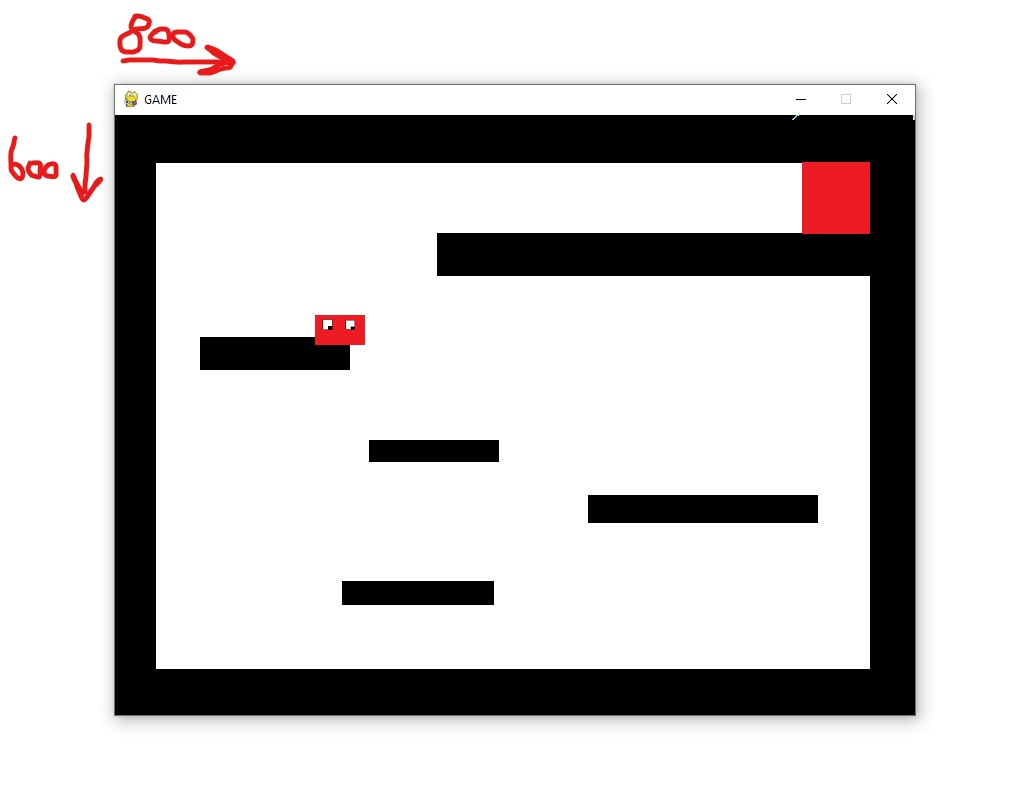
\includegraphics[width=6in, frame]{gameWindow.jpg}
    \caption{800 x 600 Game Window}
    \label{fig1}
\end{figure}

\paragraph{Test 2 and 3 (\hl{Successful} / Unsuccessful)}
Test 2 and 3 can be evidenced together, as the background image is loaded and then displayed to the game window. This test was successful as there where no errors when loading the image, and then it successfully displayed said image to the game window. This can be seen in the figure above. This also meets success criteria point 4, \textit{'4. display a background to the game window'}.

\pagebreak

\paragraph{Test 4 (\hl{Successful} / Unsuccessful)}
Test 4 was to test if the 'X' button in the top right of the game window would close the game. This is because, in pygame, there are two lines of code required for this button to work, so this test ensures the functionality of the button is in working order. The test was successful as the program was closed upon the button being pressed. I have included evidence of this below. The figure shows IDLE's method of confirming that the user wants to kill the program. This is confirmation that the 'X' button is working correctly. This also meets success criteria point 5, \textit{'5. close when the ’X’ button is pressed at any time'}.

\begin{figure}[H]
    \centering
    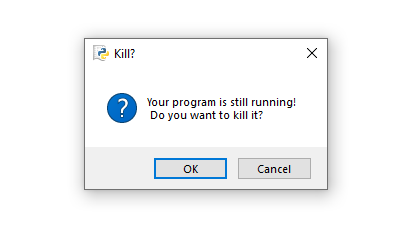
\includegraphics[width=4in, frame]{gameClose.png}
    \caption{Game Closure}
    \label{fig2}
\end{figure}

\paragraph{Test 5 (\hl{Successful} / Unsuccessful)}
Test 5 was to see if the player image would be displayed to the screen on the launch of the program. This test was successful as the player image was loaded to the screen on start up. The image was loaded to a position that was pre-defined in the code. For example, the \textit{x} and \textit{y} values determine where the player will start, and then any updates made will increase/decrease these values. I have included a figure of the player image being displayed to the game window. This also meets the first part of success criteria 3, \textit{'3. display a working player model...' }.

\begin{figure}[H]
    \centering
    
\includegraphics[width=3in, frame]{playerFig.png}
    \caption{Player Character}
    \label{fig3}
\end{figure}

\pagebreak

\paragraph{Test 6 and 7 (\hl{Successful} / Unsuccessful)}
Test 6 and 7 where to test if the player can move in the \textit{x} or \textit{y} direction. This test was successful as my player moved in both the \textit{x} and \textit{y} direction smoothly with no errors. The player can even move diagonally when two keys are pressed as the same time. This meets success criteria point 3, \textit{'3. display a working player model with basic movement...'}. I have included a figure of the debug panel showing when key presses are registered as evidence.

\begin{figure}[H]
    \centering
    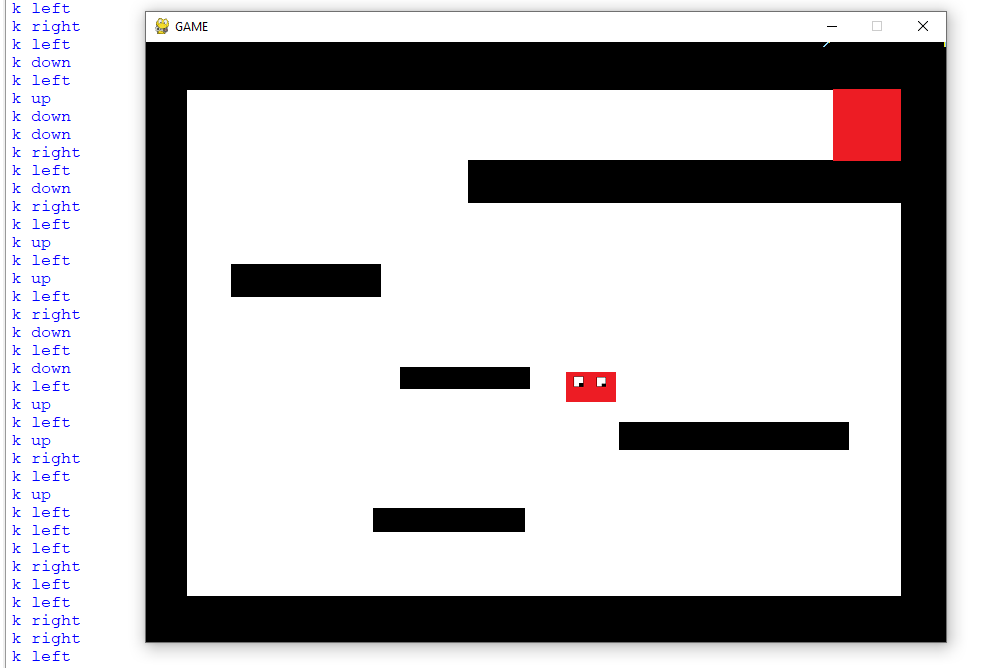
\includegraphics[width=6in, frame]{playerMovement.png}
    \caption{Player Movement}
    \label{fig4}
\end{figure}

\paragraph{Summary of Testing}
The testing for iteration was as successful as possible. Every test I set to preform at the start of iteration 1 was conducted and each test was successful in its own right. Each test provided evidence that the success criteria had been consistently met, as may tests could be linked back to said criteria. I will be discussing the success of the iteration as a whole in the iteration 1 evaluation below.

\pagebreak

\section{Comments and Maintainability}
Throughout this iteration, I have also been using comments within Python to maintain my program code. These can be made in Python by using a '\#' to denote any text after, on the same line, is within the comment. Comments are useful as they give a brief description of the functionality of either a line or section of code. I have used them as they will help me remember what my program code does in the future. I have included some examples from my code below.

\begin{figure}[H]
     \centering
    \subfigure[Comments - Movement]{
    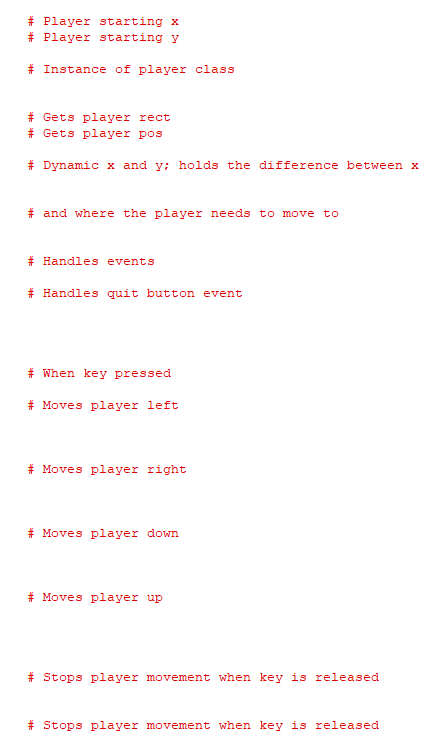
\includegraphics[width=2.85in, frame]{comments1.png}
    }
    \subfigure[Comments - Updates ]{
    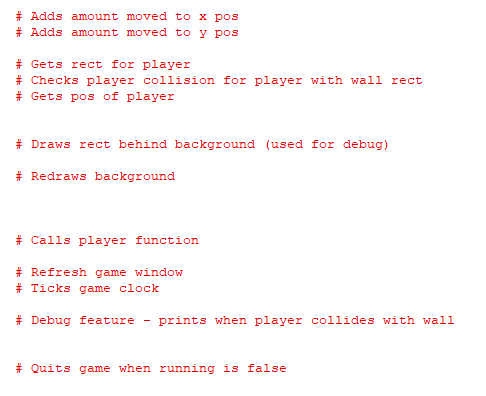
\includegraphics[width=2.85in, frame]{comments2.png}
    }
    \caption{Iteration 1 Comments}
\end{figure}

\pagebreak

\section{Iteration 1 Evaluation}
In iteration one I created the basic fundamentals of a simple windowed program in pygame. I first started by creating the game window. This was a 600 x 800 pixel window with an 'X' button, so that the program could be closed at any time. I then set about displaying a background image to the screen. This background was a simple mock level that I created. This is to demonstrate what the levels will look like in future iterations. After successfully implementing this background image, I began to set about creating a moving character for the player to control. 
\newline
\newline
I started this character creation process with displaying the player image to the screen. I did this by loading the image and creating an update loop in which the image was displayed to the screen, 60 times per second. This is the frame rate of the game. I then implemented basic multi-directional movement to the character. This allows the player to move smoothly around the screen. I think that I implemented this into my program successfully as there is no issues with the character movement.
\newline
\newline
I then attempted to implement collision between the player and the four walls of the game window. I did manage to implement collision in one plain, however I struggled to do so for all directions. This is something that I need to fix in iteration 2.
\newline
\newline
Overall, I succeeded in creating the basic foundations of my program. I spent a lot of my time learning over the course of this iteration, especially to do with the logic behind moving the player. I think I have met most of the success criteria, whilst also developing a greater understanding of how I can implement more features in the future. I have met all of the points set in the success criteria at the start of this iteration, with the only exception being the player having basic collision with the environment. I did meet this criteria to a partial level, however work is needed in iteration two, to ensure this mechanic is fully developed.  

\pagebreak

\section{Stakeholder Conversation}
After finishing the first iteration, I contacted my stakeholder to let them know I was ready for their feedback. In summary, my stakeholder was pleased with the fundamentals, but would like to see a significant amount of development in iteration two. They stated that they would like to see multiple levels moving forward, with the implementation of walls, with working coalition between them and the player. My stakeholder also stated that they would like to see 'a more diverse level set', so my main focus will be creating a wide range of levels for the user to navigate. I have included my stakeholders email below. 

\begin{figure}[H]
    \centering
    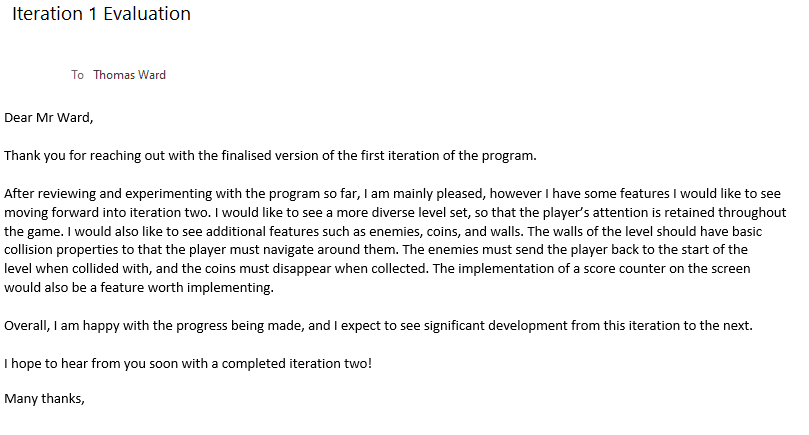
\includegraphics[width=6in, frame]{stakeholder iteration 1.PNG}
    \caption{Stakeholder Iteration 1 Feedback}
    \label{stakeholder4}
\end{figure}

\section{Next Steps}
Moving forward with the development of this program, I will be focusing on developing the world environment. The main focus of iteration two will be on creating multiple levels for the user to explore. This will be done by reading a grid-like data set from an external file. This data will then be used to relate certain values to blocks in which can be placed around the level. This will make levels easy to add and also allow for a wide range of customisation.  

\chapter{Iteration 2}

\begin{figure}[H]
    \centering
    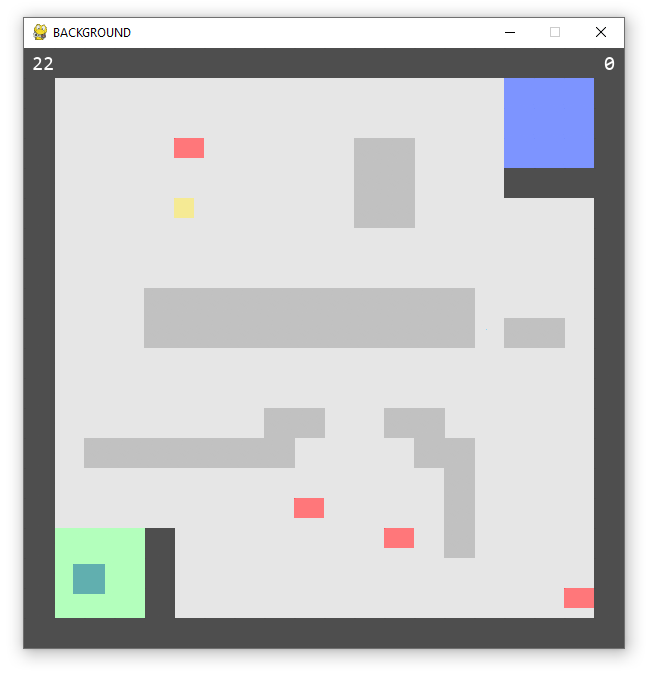
\includegraphics[width=5in]{iteration2title.png}
    \label{iteration2title}
\end{figure}

\section{Introduction}
Over the course of iteration 2, I will be developing a level system for the program, which will retrieve data from external files. I will also be adding smaller elements to each level, such as enemies, a score system using collectable coins, and a level timer. Firstly, I will be fixing the players collision system, and then I will be adapting this to include player collisions with the level walls, enemies, coins, and exit gates. A more detailed list of aims for this iteration will be provided below in the success criteria for this iteration. 

\section{Iteration 2 Success Criteria}
Throughout iteration 2, I will be aiming to implement:

\begin{enumerate}
    \item working collisions between the player and level environment.
    \item a score counter, which is incremented every time a player collides with a coin, onto the screen at all times.
    \item a timer for each level.
    \item basic conditional text screens i.e. when the player has ran out of time or completed the game.
    \item sound effects for collisions such as with an enemy, with a coin, or the exit gate.
    \item a wide range of custom levels, with all level data stored in a 'levels' folder.
    \item a grid-like level layout, with each block-type having a unique and identifiable texture.
    \item the player is reset to the start when they collide with an enemy.
\end{enumerate}

\paragraph{Why?} I will be using this small success criteria to refer back to throughout iteration 2. I will use it to ensure I meet the key goals within this version. This success criteria is also based off the feedback provided to me by my stakeholder. This means if I follow this criteria, my stakeholder will be pleased with the outcome of iteration 2.

\pagebreak

\section{Test Plan for Iteration 2}

\paragraph{What I Plan to Test}I will be testing throughout the course of iteration 2 to ensure the program is working as intended, after the implementation of each small feature. I will be testing to see if the level data is read correctly, the appropriate blocks are placed off the back of this data, the player collides correctly with the level environment, the correct sounds are played depending on the collision, and any other features I decide to implement in over the course of this iteration. 

\begin{table}[H]
    \centering
    \begin{tabular}{|c|c|c|c|}
    \hline
    \textbf{*} & \textbf{Test Description} & \textbf{Test Data} & \textbf{Expected Outcome}\\
    \hline
    1 & Player stops moving when & On collision. & The player stops moving when \\
    & collided with a wall element. & & collision is made.\\
    \hline
    2 & The level data is read & On start-up. & The data is stored in a 2D array\\
      & correctly and saved in a&             & which can be called globally. \\
      & two-dimensional array. & &\\
    \hline
    3 & Each block of the level is & 2D array. & The level data is read and appropriate\\
    & displayed according to data &           & blocks are placed across the level. \\
    & in the level map. & &\\
    \hline
    4 & A sound will play when the & On collision & The appropriate sound will play\\
    & player interacts with enemies, & & when the player collides with any  \\
    & coins, or the exit gate. & & of these.\\
    \hline
    5 & The next level will be loaded & On collision. & The program will display the \\
    & and displayed onto the game & & correct level to the screen. \\
    & window. & & \\
    \hline
    6 & The score counter should & On collision & The score counter will increase\\
    & increment when a coin is & & when a coin is collected.\\
    & collected. & & \\
    \hline
    7 & The player must reset when & On collision & The player will reset back to\\
    & collided with an enemy. & & the start of the level.\\
    \hline
    8 & A text screen will appear if & On event. & A text screen should appear with the \\
      & the player runs out of time & & relevant information for the user for \\
      & or completes the game. & & at least 5 seconds.  \\
    \hline
    \end{tabular}
    \caption{Iteration 2 Pre-Development Testing Plan}
    \label{TestTable}
\end{table}

\pagebreak

\section{Code Development}
I will be displaying the newly implemented sections of my code below, and also justifying why I have made certain decisions. I will be explaining how I have adapted my program to include these new features. 

\subsection{Updated Player Class}
I have updated the player class to include the movement of the player, as well as the collision detection. Displayed below is the code for the player collision with the level environment. The program checks if the player rect has collided with a tile, if so the player is stopped. This is done by using a built-in function of pygame, \textit{collide.rect}. The collision for the exit gate is done in a similar way, however when a collision is detected, the \textit{next\_level} variable is set to true. The program then runs the code to increment the level accordingly. The code for this will be displayed along with the world class below. I have designed the program in this was as it was the most efficient way I could find to implement a fully working collision system. This way of programming is also scale-able as new collisions can be easily added below.

\begin{Verbatim}[numbers=left, frame=single]
for tile in world.tile_list:
    if tile[1].colliderect(self.rect.x+dx,
                           self.rect.y,
                           self.width,
                           self.height):
        dx = 0

    if tile[1].colliderect(self.rect.x,
                           self.rect.y+dy,
                           self.width,
                           self.height):
        dy = 0

    if pygame.sprite.spritecollide(self,exit_group,False):
        nextLevel_sound.play()
        next_level = True

    if pygame.sprite.spritecollide(self,enemy_group,False):
        death_sound.play()
        reset(level,world_data,world)

    self.rect.x += dx
    self.rect.y += dy
    gameDisplay.blit(self.player1_img, self.rect)
    return next_level
\end{Verbatim}



\pagebreak

\subsection{The Level System}
\subsubsection{The World Class}

\begin{Verbatim}[numbers=left, frame=single]
class World():
    def __init__(self,data):
        self.tile_list = []
        wall = pygame.image.load("img/TEXTURE1.png")                                   
        light_wall = pygame.image.load("img/TEXTURE2.png")
        row_count = 0
        for row in data:
            col_count = 0
            for tile in row:
                if tile == "1":
                    img = pygame.transform.scale(wall, 
                                (tile_size, tile_size))
                    img_rect = img.get_rect()
                    img_rect.x = col_count * tile_size
                    img_rect.y = row_count * tile_size
                    tile = (img, img_rect)
                    self.tile_list.append(tile)
                if tile == "2":
                    img = pygame.transform.scale(light_wall,
                                (tile_size + 1,tile_size))
                    img_rect = img.get_rect()
                    img_rect.x = col_count * tile_size
                    img_rect.y = row_count * tile_size 
                    tile = (img, img_rect)
                    self.tile_list.append(tile)
                if tile == "3":
                    start = Start((col_count*tile_size) + 1,
                                   row_count*tile_size)
                    start_group.add(start)
                if tile == "4":
-                   exit = Exit(col_count * tile_size,
                                row_count * tile_size)
                    exit_group.add(exit)
                if tile == "5":
                    enemy = Enemy(col_count * tile_size,
                                 row_count * tile_size)
                    enemy_group.add(enemy)
                if tile == "6":
                    coin = Coin(col_count * tile_size,
                                row_count * tile_size)
                    coin_group.add(coin)
\end{Verbatim}

\pagebreak

This is the world class. I have implemented this class in iteration two as it allows me to create a tile-base level system, with room for scale-ability. The world class works by taking the data stored in a two-dimensional array called \textit{data}. The class then iterates through this data, each time checking the value of each item. The tile maps work by storing values from 1-6 in a grid-like way. This then indicates to the program which texture/attributes each block should have. I have done this because it is a very straight-forward way of creating complex levels within my program. An example is provided below. 

\subsubsection{The World Data}

\begin{Verbatim}[numbers=left, frame=single]
1 1 1 1 1 1 1 1 1 1 1 1 1 1 1 1 1 1 1 1
1 0 0 0 0 0 0 0 0 0 0 0 0 0 0 0 4 4 4 1
1 0 0 0 0 0 0 0 0 0 0 0 0 0 0 0 4 4 4 1
1 0 0 0 0 5 0 0 0 0 0 2 2 0 0 0 4 4 4 1
1 0 0 0 0 0 0 0 0 0 0 2 2 0 0 0 1 1 1 1
1 0 0 0 0 6 0 0 0 0 0 2 2 0 0 0 0 0 0 1
1 0 0 0 0 0 0 0 0 0 0 0 0 0 0 0 0 0 0 1
1 0 0 0 0 0 0 0 0 0 0 0 0 0 0 0 0 0 0 1
1 0 0 0 2 2 2 2 2 2 2 2 2 2 2 0 0 0 0 1
1 0 0 0 2 2 2 2 2 2 2 2 2 2 2 0 2 2 0 1
1 0 0 0 0 0 0 0 0 0 0 0 0 0 0 0 0 0 0 1
1 0 0 0 0 0 0 0 0 0 0 0 0 0 0 0 0 0 0 1
1 0 0 0 0 0 0 0 2 2 0 0 2 2 0 0 0 0 0 1
1 0 2 2 2 2 2 2 2 0 0 0 0 2 2 0 0 0 0 1
1 0 0 0 0 0 6 0 0 0 0 0 0 0 2 0 0 0 0 1
1 0 0 0 0 0 0 0 0 5 0 0 0 0 2 0 0 0 0 1
1 3 3 3 1 0 0 0 0 0 0 0 5 0 2 0 0 0 0 1
1 3 3 3 1 0 0 0 0 0 0 0 0 0 0 0 0 0 0 1
1 3 3 3 1 0 0 0 0 0 0 0 0 0 0 0 0 0 5 1
1 1 1 1 1 1 1 1 1 1 1 1 1 1 1 1 1 1 1 1
\end{Verbatim}

This is the tile map for the first level of my solution so far. I have laid the data out this way within the text file to visualise the level grid. This allows for the levels to be easily modified if needed. This grid is 20 x 20 and allows for detailed levels to be made. The program is designed to read these level data files sequentially, depending on which level the player is currently on. \newline

The player class then takes this data and iterates through the array. The tiles are placed onto the level so that the user can interact with the environment. Each tile is then scaled appropriately. I have done this so the wall elements fit the resolution of the game window. The scaling of each tile is also used to make coins and enemies smaller than a single tile. I have done this so the player can easily identify an enemy or a coin via its unique shape/size. 

\pagebreak

\subsubsection{The Reset Function}
The reset function handles the event of the player reaching the exit gate. When the player does so, all the current level data is wiped from the screen. The next level is then loaded and displayed to the game window. The player is also reset back to the start gate. I have designed this function in this way as it can be used at any point throughout my program. This means that the level can be incremented or reset at any time, or depending on certain conditions. This can also be used for resetting the world if a player collides with an enemy. This is because the level data passed in will be the current level if the player interacts with an enemy, or the next level data if the player collides with the exit gate. There is also a draw method for this world class. \footnote{Draw method located in the appendix. Page \pageref{appendix}.}

\begin{Verbatim}[numbers=left, frame=single]
def reset(level,world_data,world):
    p1.reset(49, 516)
    start_group.empty()
    exit_group.empty()
    enemy_group.empty()
    coin_group.empty()
    
    with open(f"levels/level_{level}.txt") as textFile:
        world_data = [line.split() for line in textFile]
    world = World(world_data)
    
    return world
\end{Verbatim}

\subsubsection{Initialising the First Level}
Before the reset function is called, the program first needs to display the first level to the screen. I have added the code for loading the level just before the game loop. I will display the code for this feature below. I have done this because the player needs to attempt the level in-order to provide a instance in which the reset function is needed i.e. colliding with an enemy. \label{draw method}

\begin{Verbatim}[numbers=left, frame=single]
with open(f"levels/level_{level}.txt") as textFile:
    world_data = [line.split() for line in textFile]
\end{Verbatim}

As you can see, this is the same code used above in the reset function. This is because the world is loaded in the same way. This code loads the world data from the appropriate text file and stores it in the two-dimensional array \textit{world\_data}.

\pagebreak

\subsection{Sprite Classes}
These are the classes in which store the basic attributes of each sprite. The sprites are tiles such as coins and enemies. I have made these objects sprites as it makes collisions simpler. It also optimizes my program as it saves writing repeated lines of code. This was a time-saving benefit when designing my program.

\subsubsection{The Start Class}


\begin{Verbatim}[numbers=left, frame=single]
class Start(pygame.sprite.Sprite):
    def __init__(self,x,y):
            pygame.sprite.Sprite.__init__(self)
            img = pygame.image.load("img/TEXTURE3.png")
            self.image = pygame.transform.scale(img, 
                                               (tile_size,tile_size))
            self.rect = self.image.get_rect()
            self.rect.x = x
            self.rect.y = y
\end{Verbatim}

\subsubsection{The Exit Class}


\begin{Verbatim}[numbers=left, frame=single]
class Exit(pygame.sprite.Sprite):
    def __init__(self,x,y):
            pygame.sprite.Sprite.__init__(self)
            img = pygame.image.load("img/TEXTURE4.png")
            self.image = pygame.transform.scale(img,
                                               (tile_size,tile_size))
            self.rect = self.image.get_rect()
            self.rect.x = x
            self.rect.y = y
\end{Verbatim}

\subsubsection{The Enemy Class}


\begin{Verbatim}[numbers=left, frame=single]
class Enemy(pygame.sprite.Sprite):
    def __init__(self,x,y):
        pygame.sprite.Sprite.__init__(self)
        img = pygame.image.load("img/TEXTURE5.png")
        self.image = pygame.transform.scale(img,
                                        (tile_size, tile_size - 10))
        self.rect = self.image.get_rect()
        self.rect.x = x
        self.rect.y = y
\end{Verbatim}

\subsubsection{The Coin Class}


\begin{Verbatim}[numbers=left, frame=single]
class Coin(pygame.sprite.Sprite):
    def __init__(self,x,y):
        pygame.sprite.Sprite.__init__(self)
        img = pygame.image.load("img/TEXTURE6.png")
        self.image = pygame.transform.scale(img, 
                                           (tile_size - 10,
                                           tile_size - 10))
        self.rect = self.image.get_rect()
        self.rect.x = x
        self.rect.y = y
\end{Verbatim}

Having the attributes stored in this object-orientated way also allows for methods to be added in the future. I kept this in mind when designing the program this way. This means that an attribute could be added to the enemy class in which allows the enemy to move on either a horizontal or vertical plane. Any other future tiles to be added can be designed in the same way and implemented with ease. This gives my program a modular structure with room for lots of future development. 

\subsection{Game Sounds}
I have added sounds to my game in this iteration. This is so that the player has a well rounded experience whilst playing. It also give audio queues to players when they have collected a coin, collided with an enemy, ran out of time, or completed the game. This makes the game feel more immersive and will entice the attention of the users further. I will display the code for these sound effects below. I have also added background music to the program to again enhance the user experience whilst playing. 

\begin{Verbatim}[numbers=left, frame=single]
pygame.mixer.music.load("sounds/background_music.wav")
pygame.mixer.music.play(-1)
coin_sound = pygame.mixer.Sound("sounds/coin_collect.wav")
death_sound = pygame.mixer.Sound("sounds/death.wav")
nextLevel_sound = pygame.mixer.Sound("sounds/nextLevel.wav")
win_sound = pygame.mixer.Sound("sounds/win.wav")
\end{Verbatim}

Playing the sounds:

\begin{Verbatim}[numbers=left, frame=single]
nextLevel_sound.play()
death_sound.play()
coin_sound.play()
win_sound.play()
\end{Verbatim}

\pagebreak
 
\section{Screenshots of Game-Play}
 I have included screenshots of the game being played, so that you can see what the program looks like between levels. Level 1, 2 and 3 have been displayed below, along with the screen that is displayed when you win. I have shown the win screen as it is a basic text screen. I have done this as screens like this will be used throughout my game to display information to the user.
 
 
 \begin{figure}[H]
    \subfigure[Fig.a]{
    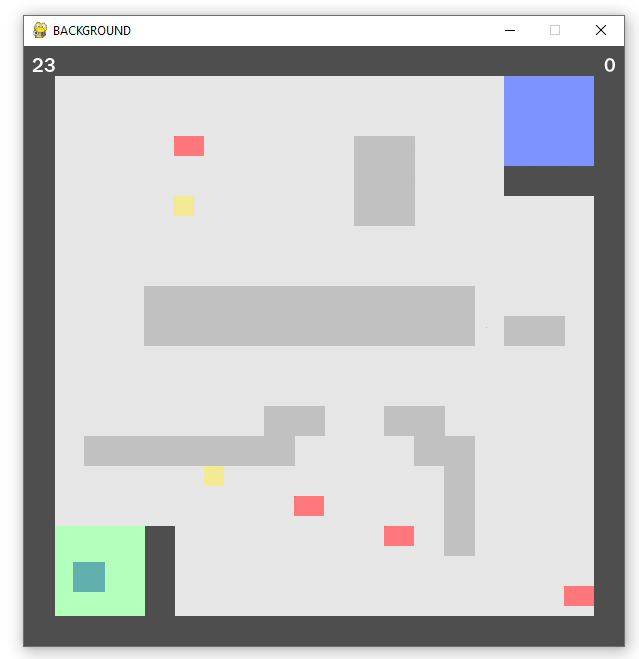
\includegraphics[width=3in, frame]{iteration2gameplay1.PNG}
    }
    \subfigure[Fig.b]{
    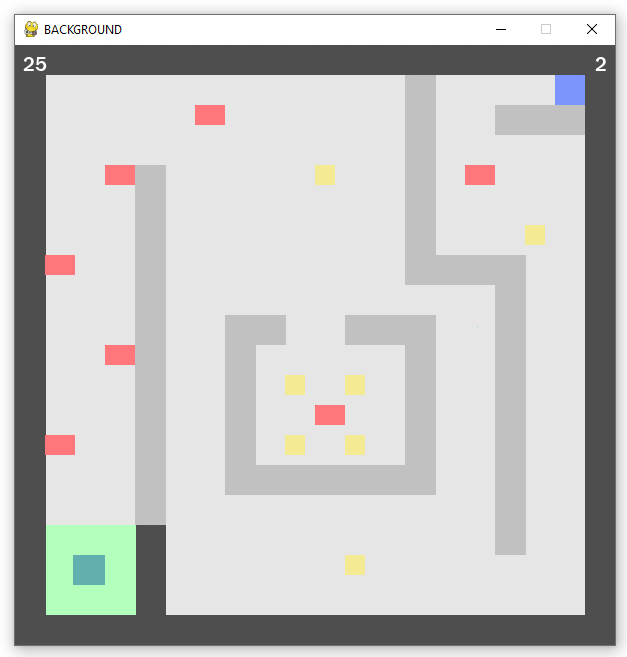
\includegraphics[width=3in, frame]{iteration2gameplay2.PNG}
    }
    \subfigure[Fig.c]{
    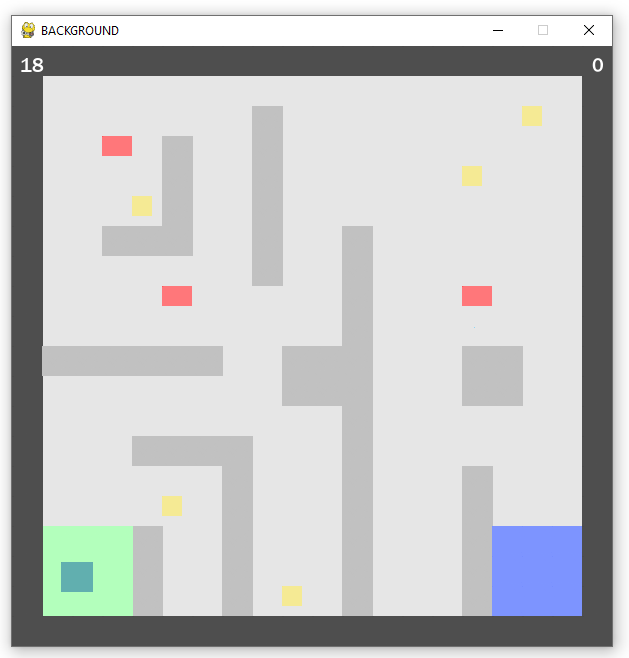
\includegraphics[width=3in, frame]{iteration2gameplay3.PNG}
    }
    \subfigure[Fig.d]{
    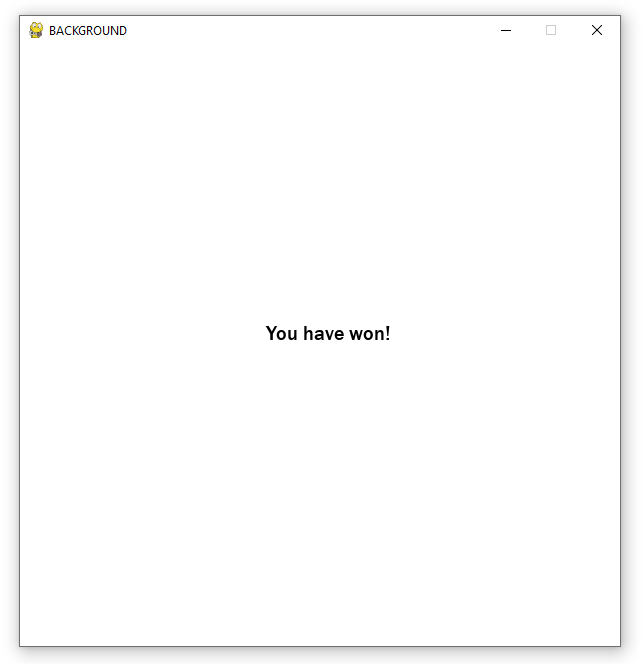
\includegraphics[width=3in, frame]{iteration2gameplay4.PNG}
    }
    \caption{Iteration 2 Game-play}
\end{figure}
 
\pagebreak
 
\section{Post-Development Testing}
Here is the original test plan for iteration 2. I have included this to reference back to when competing my post development testing. I will be completing each test, and the discussing whether the test was successful or not.

\begin{table}[H]
    \centering
    \begin{tabular}{|c|c|c|c|}
    \hline
    \textbf{*} & \textbf{Test Description} & \textbf{Test Data} & \textbf{Expected Outcome}\\
    \hline
    1 & Player stops moving when & On collision. & The player stops moving when \\
    & collided with a wall element. & & collision is made.\\
    \hline
    2 & The level data is read & On start-up. & The data is stored in a 2D array\\
      & correctly and saved in a&             & which can be called globally. \\
      & two-dimensional array. & &\\
    \hline
    3 & Each block of the level is & 2D array. & The level data is read and appropriate\\
    & displayed according to data &           & blocks are placed across the level. \\
    & in the level map. & &\\
    \hline
    4 & A sound will play when the & On collision & The appropriate sound will play\\
    & player interacts with enemies, & & when the player collides with any  \\
    & coins, or the exit gate. & & of these.\\
    \hline
    5 & The next level will be loaded & On collision. & The program will display the \\
    & and displayed onto the game & & correct level to the screen. \\
    & window. & & \\
    \hline
    6 & The score counter should & On collision & The score counter will increase\\
    & increment when a coin is & & when a coin is collected.\\
    & collected. & & \\
    \hline
    7 & The player must reset when & On collision & The player will reset back to\\
    & collided with an enemy. & & the start of the level.\\
    \hline
    8 & A text screen will appear if & On event. & A text screen should appear with the \\
      & the player runs out of time & & relevant information for the user for \\
      & or completes the game. & & at least 5 seconds.  \\
    \hline
    \end{tabular}
    \caption{Iteration 2 Post-Development Testing Plan}
    \label{TestTable}
\end{table}

\paragraph{Test 1 (\hl{Successful} / Unsuccessful)}
Test 1 was to test the if the collisions between the player and level environment where working. I used a black box testing approach for test 1 as this was a test that needed to be carried out within the game itself. I began with testing the horizontal collision between the player and the generated level. I found that the horizontal collision stopped the player from moving, however the player would stop around 5 pixels before making contact with the wall. To resolve this issue, I adjusted the hit box of the tiles and tested the program again. This resolved the issue so I moved onto testing the vertical collision. After testing the vertical collision in the same way, no issues where found. The player stopped when colliding with a wall and did not overlap or stop to short of the wall texture. This created a fully-functional collision system in which improves the play-ability of the game significantly. Overall, test 1 was successfully as the predicted outcome was fulfilled to a high standard. I will include a screenshot below to evidence this. Test 1 also proved my game met success criteria point 1.

\pagebreak 

\begin{figure}[H]
    \centering
    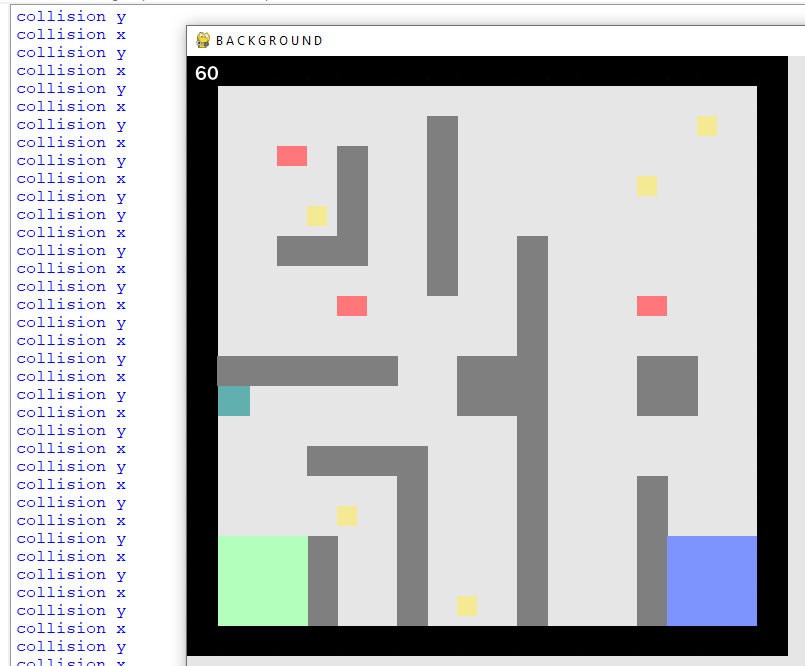
\includegraphics[width=5.5in, frame]{iteration2test1.PNG}
    \caption{Player Collision}
\end{figure}

\paragraph{Test 2 (\hl{Successful} / Unsuccessful)}
Test 2 was to test if the level data was accurately read from the level file, and then saved to a two-dimensional array within the program. I tested this by creating a function to import the data from the external file, and then printed the result. The program returned a two-dimensional array correctly, with each row of data being placed inside an array within the two-dimensional array. The level data file contains a 20 x 20 grid of values 0-6. The level function splits this data into individual arrays in rows, and iterates through them to draw the level to the game window. This test was a success as the data was stored in the array correctly and as expected. This test also proved that I have partially hit point 6 of my success criteria\footnote{Success criteria point 6 - A wide range of custom levels, with the level data being stored in a 'levels' folder.} as the level data can now be stored in an external folder/files. The data also is easily changeable so can be easily manipulated and customised. I have included a screenshot of this array within my program below.  

\begin{figure}[H]
    \centering
    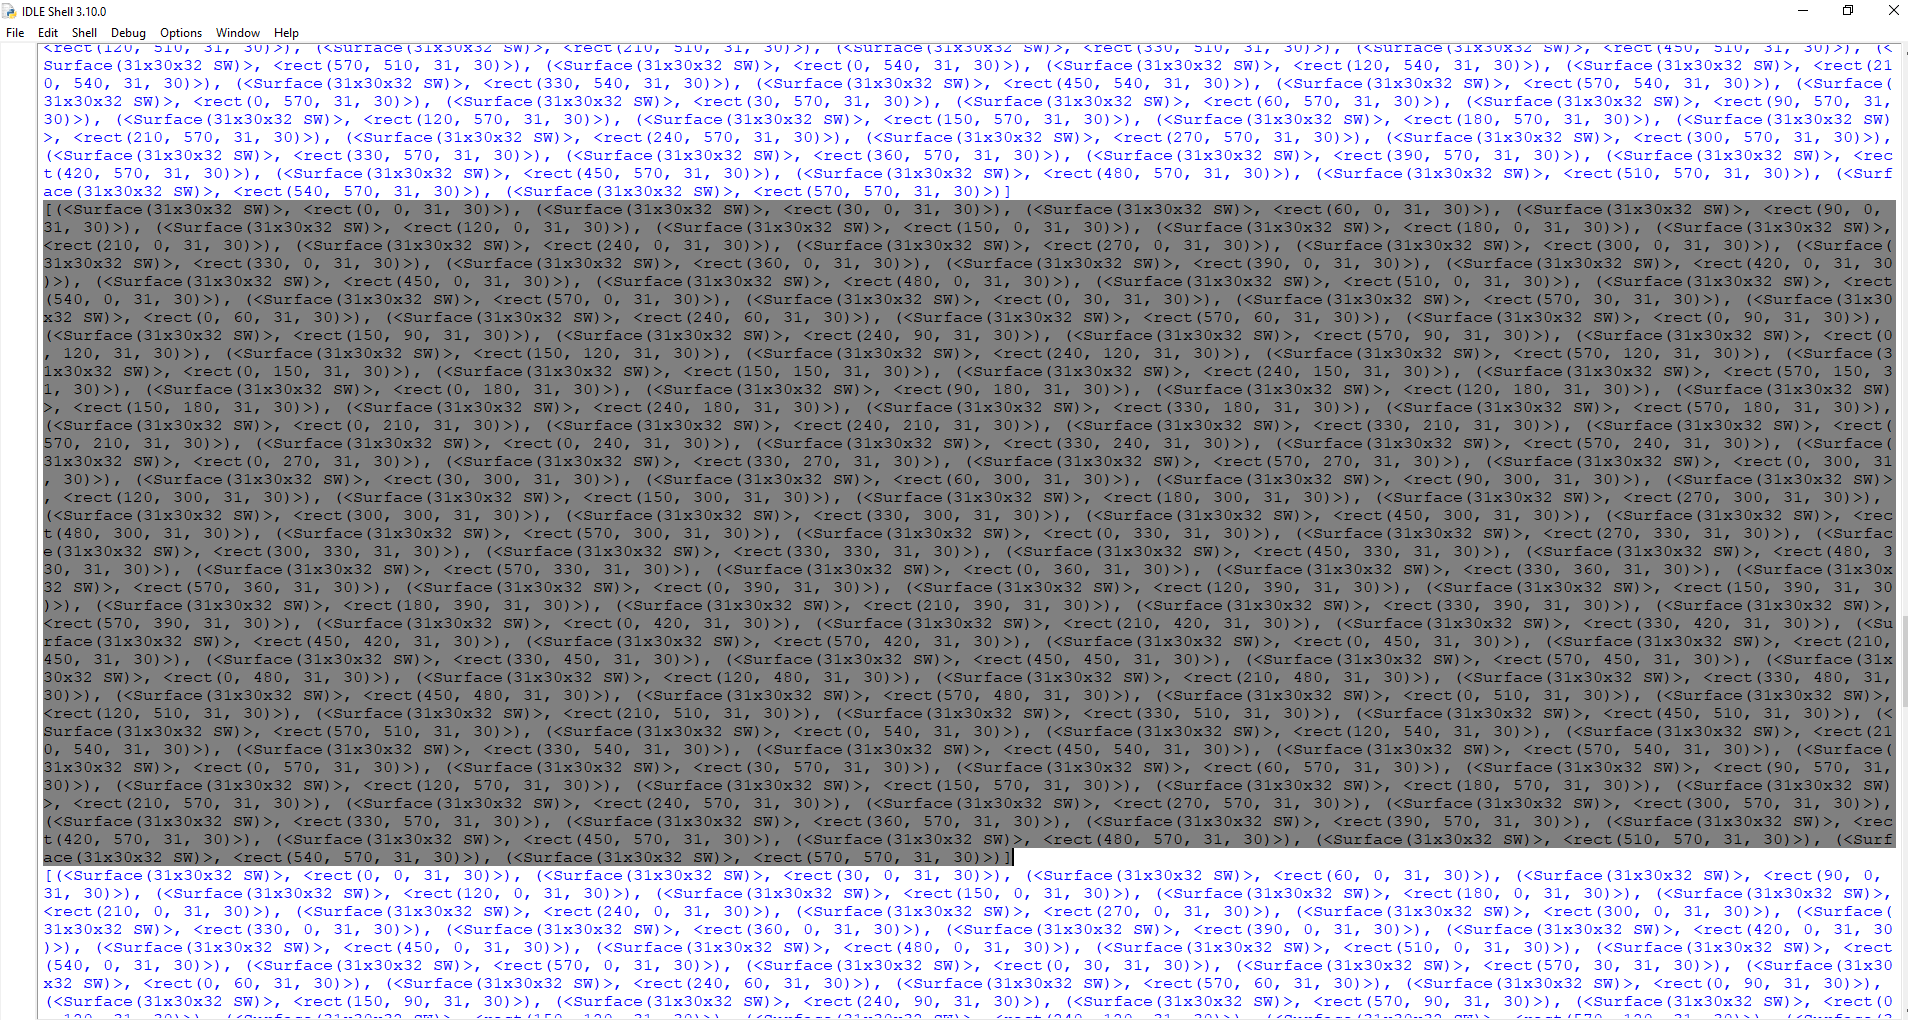
\includegraphics[width=4.75in, frame]{iteration2test2.PNG}
    \caption{Level Data Array}
\end{figure}

\paragraph{Test 3 (\hl{Successful} / Unsuccessful)}
Test 3 was to test if the level data/tile map was displayed correctly to the game window. I used a black box approach to test this feature of the game as this can only be tested when the program is running. I began with running the game and observing how the tile map was displayed to the game window. Initially, I was pleased with the way the tile map was displayed as there where no obvious errors. To test this further, I tried the collision; this was also in working order. The only adjustment I had to make to the tile map is the aforementioned reason of the player collision being around 5 pixels off on the right edge.Apart from this minor tweak, test 3 was successful and had returned the expected outcome. This test also proves that I have successfully fulfilled success criteria point 7 as the grid-like level system functioned appropriately and to a high standard. I will evidence this below,

\begin{figure}[H]
    \centering
    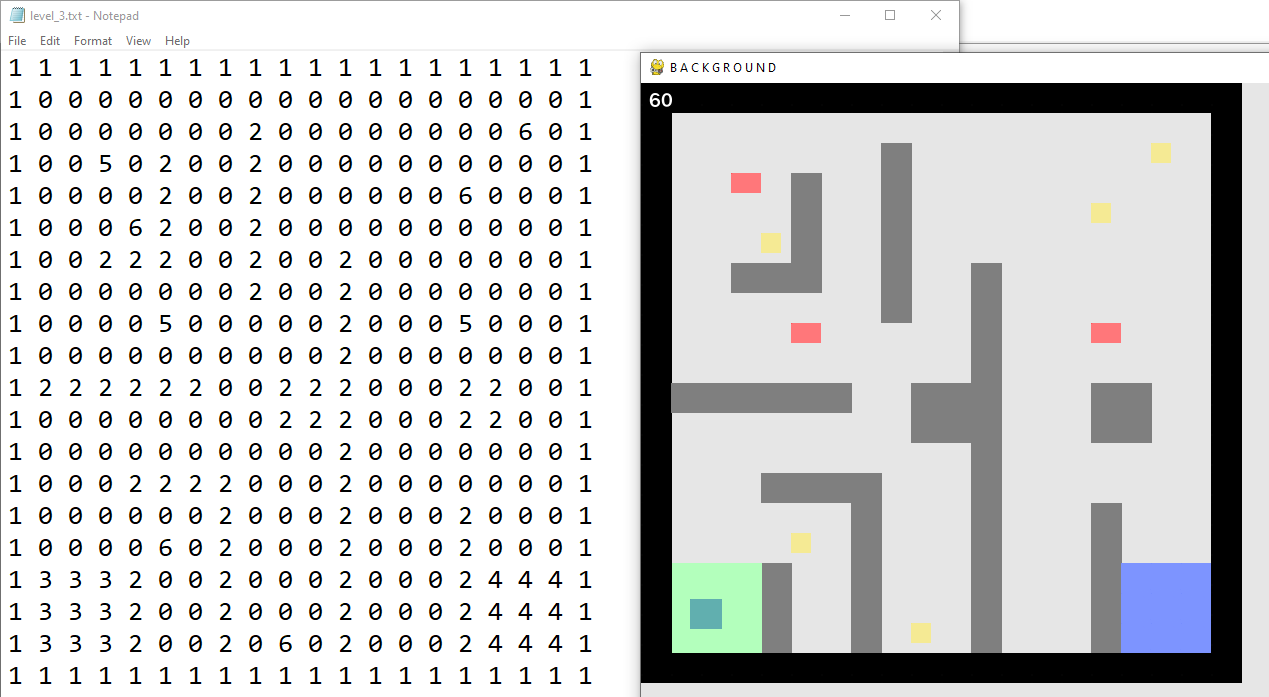
\includegraphics[width=5.25in, frame]{iteration2test3.PNG}
    \caption{Tile Map Level System}
\end{figure}

\paragraph{Test 4 (\hl{Successful} / Unsuccessful)}
Test 4 was to test if the sounds within my game played when the player would interact with a level object such as a coin or enemy. I used a black box approach to test this as I need to play the game in the game window to hear the sounds. I started by collecting a coin to see if the coin collection noise would play. The noise played when I collected the coin every time this test was carried out. I then moved onto testing the enemy collision sound. The same expected outcome was returned when testing this sound effect. The sound played correctly. I also programmed this sound to play when the player ran out of time. These sounds played at the correct time, as stated in the expected outcome. I have also hit success criteria point 5\footnote{Success criteria point 5 - Sound effects for collisions such as with an enemy, with a coin, or the exit gate.}.

\paragraph{Test 5 (\hl{Successful} / Unsuccessful)}
Test 5 was to see if the next level level was loaded when the player interacted with the end gate. I used a black box testing approach to test if this feature works correctly as it needed to be tested through the game window. I began with trying to progress to the next level. This feature worked with no flaws across all levels. I even tried implementing new levels and the exit gate tile worked with no errors. I added a short sound effect to let the player know they have move onto the next level. The expected outcome of this test was found straight away. This test also proves that the program has hit success criteria point 6\footnote{Success Criteria point 6 - A wide range of custom levels, with all level data stored in a ’levels’ folder.} successfully, as the player can progress onto the next level. 

\paragraph{Test 6 (\hl{Successful} / Unsuccessful)}
Test 6 was to see if the score counter incremented every-time a coin was collected. I have added coins as it adds a score/competitive element to the game. The collision between the player and the coin tile worked correctly, with the coin being removed from the screen when collided with. After being collected, the score variable was incremented and the correct value was displayed in the top right corner of the game window. The coins reset whenever the player had died. This meant more coins could be collected this way, so this is an issue to fix in iteration 3. This test proves that I have hit success criteria point 2\footnote{ Success criteria point 2 - a score counter, which is incremented every time a player collides with a coin, onto the screen at all times.}. 

\begin{figure}[H]
    \centering
    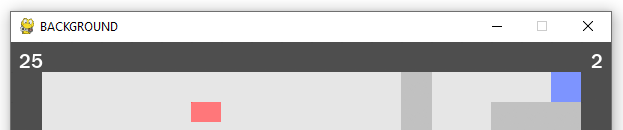
\includegraphics[width=\linewidth, frame]{iteration2test6.PNG}
    \caption{Score Counter}
\end{figure}

\pagebreak

\paragraph{Test 7 (\hl{Successful} / Unsuccessful)}
Test 7 was to test if the player was reset to the beginning after colliding with an enemy. I again used a black box approach to testing this as this could not be tested by looking through the program code. I began by loading the program and moving the enemy into an enemy. Once the player had collided with the enemy sprite, the player was sent back to the start gate. This was the expected outcome of this test and has also proved I have hit success criteria point 8\footnote{Success Criteria point 8 - the player is reset to the start when they collide with an enemy.}.

\paragraph{Test 8 (\hl{Successful} / Unsuccessful)}
Test 8 was to test if the text screens I have implemented will display, depending on the event. For example, when the player runs out of time, a screen will appear telling the player this. I began by checking the code; there where no obvious errors. I then moved on to a black box testing approach. I began by setting the level timer to 3 seconds to increase the efficiency of my testing, and then waited for the timer to reach 0. The correct screen was displayed and the player was forced to restart the program. This was the expected outcome of the test, thus making test 8 successful. The same test was also successful for when the player had reached the end level. I will include evidence of these two tests below. 

 \begin{figure}[H]
    \subfigure[Out of Time Screen]{
    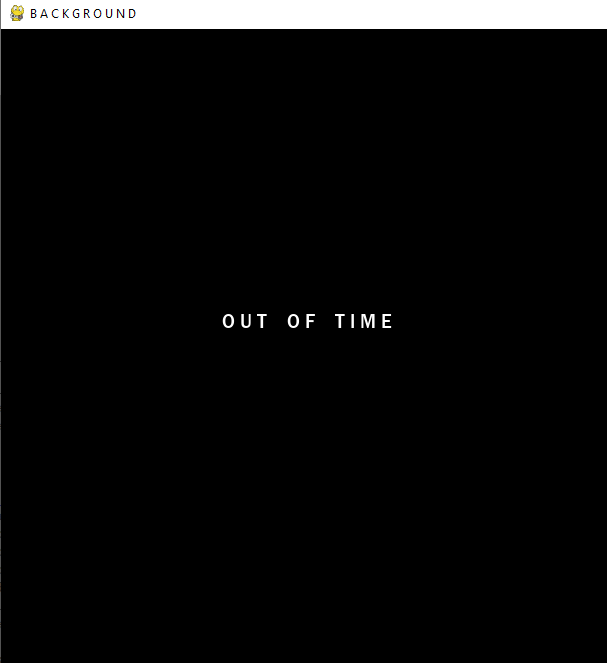
\includegraphics[width=3in, frame]{iteration2test8_1.PNG}
    }
    \subfigure[You Have Won Screen]{
    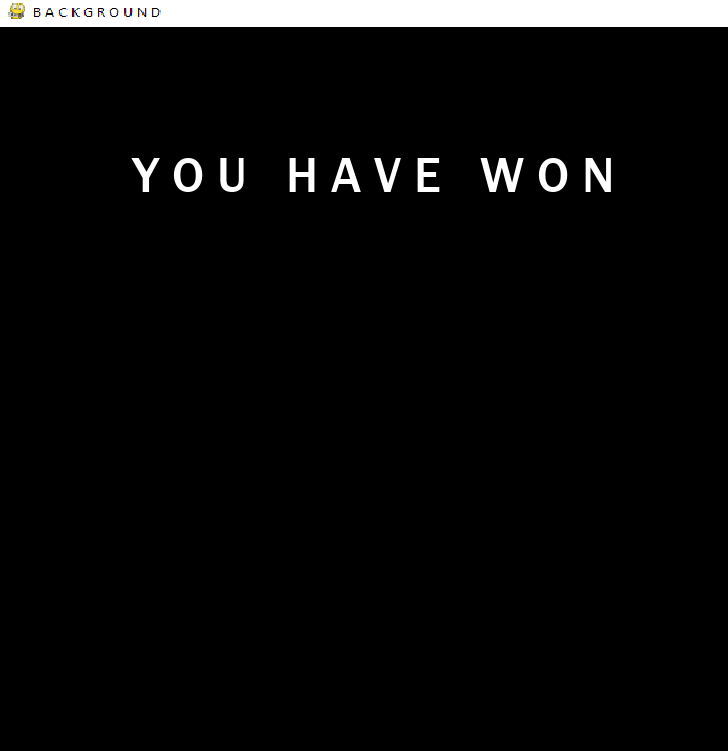
\includegraphics[width=3in, frame]{iteration2test8_2.PNG}
    }
    \caption{Text Screens}
\end{figure}

\paragraph{Summary of Testing}
Overall, each test I preformed at the end of iteration 2 development was successful and returned the expected outcome first time. This was due to the testing that was carried out along side development. As each small feature was implemented, I would test the new code to ensure it was in working order. This proved successful as the post-development testing returned the expected, successful outcome every time. 

\pagebreak

\section{Iteration 2 Evaluation}
In iteration 2, I have created a level system in which reads a tile map from an external file. The program also has multiple levels with interactive objects such as coins, enemies, and exit gates. The solution also has a level timer which requires th user to complete each level in a certain time. The program also has text scenes that pop up when the user either runs out of time or completes the game. All collisions between the player and level environment are now fully working to a high standard. The program also contains sound effects to add to the user experience whilst playing the game. All of these features have made my program a simple, yet fully functional solution to the 'game' part of my application. 
\newline
\newline
These newly implemented features are all working correctly, as proven by my testing outcomes above. I also conducted smaller tests throughout development to ensure each feature was working correctly. Each feature took a certain amount of experimentation to make work fully, but in the end each feature was fully functional.
\newline
\newline
The tile-based level system is a great addition to the program. It allows for easily customise-able levels which can be placed sequentially. This adds more of a game-like feel as well as creating a solid foundation for additional elements to be added.
\newline
\newline
I then built on this tile map to add coins and enemies. I implemented these features by placing them on the level map as a tile. This allows the elements to be placed in different locations on the map without editing the code.
\newline
\newline
I then attempted to implement pop-up questions into the program. I managed to implement a basic question system but it was not working correctly. I decided to remove this feature from the program as it was only partially working. I chose to do this as it made the program look unfinished for the end of iteration 2. This means that the stakeholder will now receive a program with features in which are fully complete. This gives the stakeholder a fully-functional solution to look and and review. 

\pagebreak

\section{Stakeholder Conversation}
After evaluating the success of iteration 2, I presented the program to my stakeholder so that they could give me feedback on the application so far. This feedback will then influence what will be done in iteration 3. I have included a screenshot of the stakeholder conversation below. 

\begin{figure}[H]
    \centering
    \includegraphics[width=\linewidth, frame]{iteration 2 stakeholder conversation.png}
    \caption{Stakeholder Iteration 2 Feedback}
\end{figure}

\section{Next Steps}
After gathering the necessary information from my stakeholder, I will now make a basic list of aims to strive towards in iteration 3. In iteration 3, I would like to aim to implement:

\begin{itemize}
    \item A question system which is triggered upon coin collection.
    \item A series of questions stored in an external data file. 
    \item A question GUI with a text box that can be typed into by the user. 
\end{itemize}

\chapter{Iteration 3}

\begin{figure}[H]
    \centering
    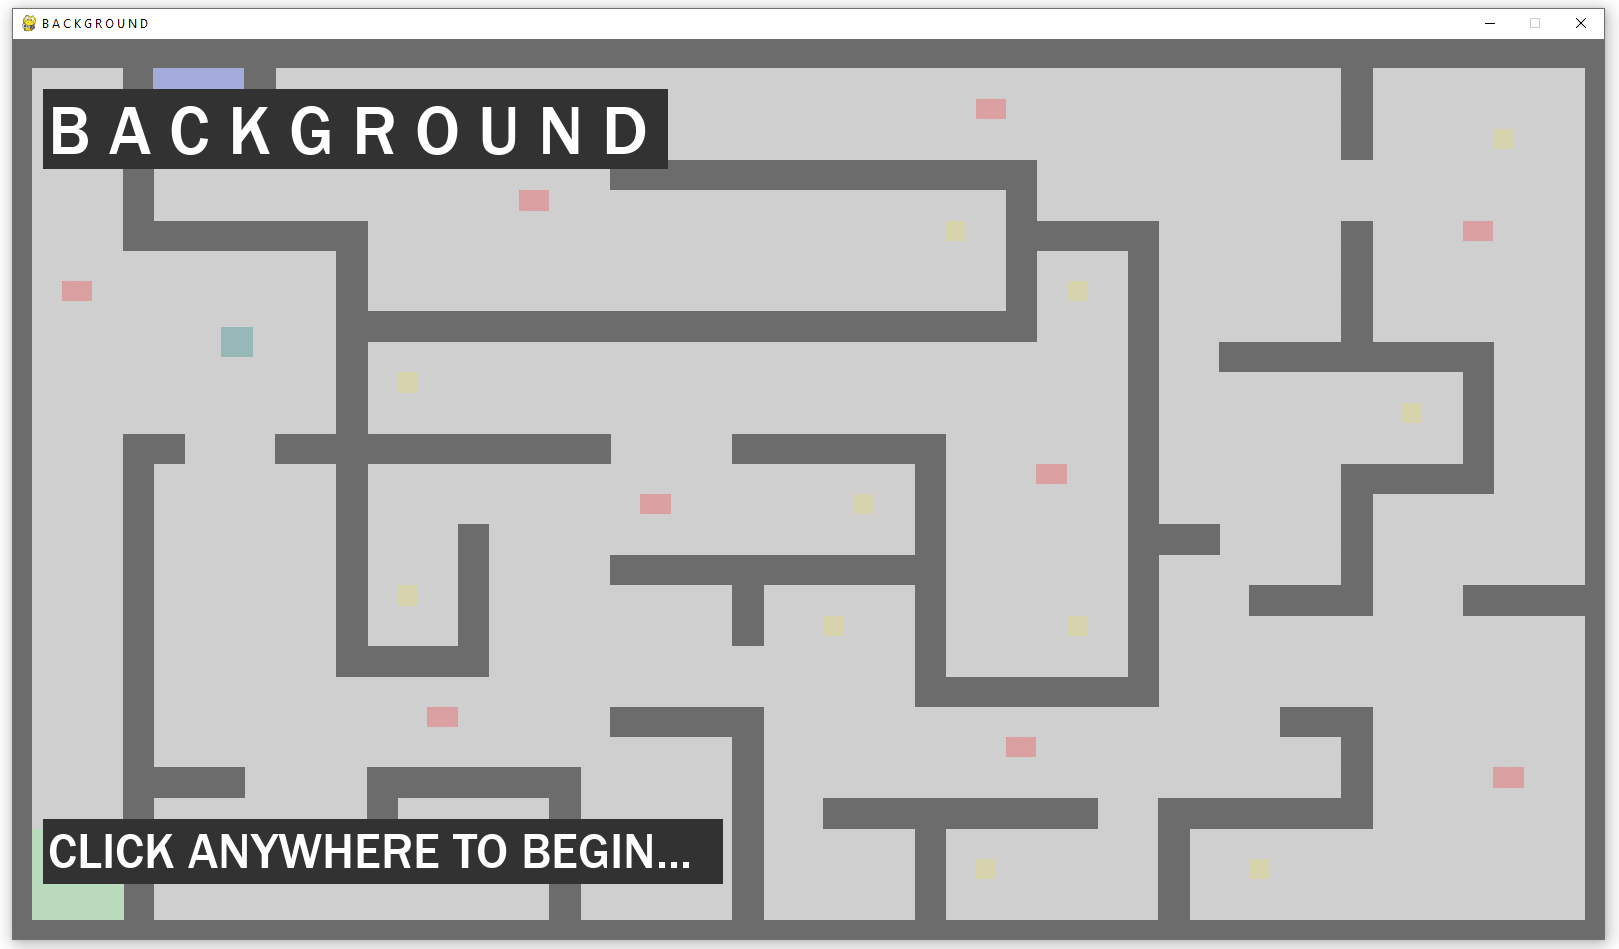
\includegraphics[width=\linewidth]{iteration3title.PNG}
\end{figure}

\pagebreak

\section{Introduction}
Over the course of iteration 3, I will be developing the menu screens as well as adding a question system. I will be doing this as my game needs to have an educational aspect. These quick fire questions will help the students remember key points regarding networks, so that they have a basic level of understating when starting year 7.

\section{Iteration 3 Success Criteria}
Throughout iteration 3, I will be aiming to implement:

\begin{enumerate}
    \item a title screen.
    \item a menu screen. 
    \item a question screen with an input box.
    \item a leader-board screen.
    \item a 'save score' screen where the user can enter their username.
    \item an end screen.
    \item working buttons for all screens.
    \item the players score is incremented when a question is answered correctly.
    \item a wider game display, with wider levels to allow for more detail per level.
    \item the updating of existing levels to match new program size.
\end{enumerate}

\paragraph{Why?}
The addition of these menu screens will make the program feel like a more completed solution. It will also allow the user to navigate the different screens with ease. The implementation of a question system will add an educational aspect to my program. This will meet the stakeholders initial requirement, which was to make the solution educational. They also suggested that I should add the educational element soon in our last conversation. The addition of a leader-board will also add a competitive element to the solution and will allow for competition between classes etc. Making the program wider and taller will allow the game to feel like an application, not just a small game in a box. This will make the users more engaged with the solution and also will allow for more detailed levels. 

\pagebreak

\section{Test Plan for Iteration 3}

\paragraph{What I Plan to Test}
In iteration 3, I will be testing if each screen, i.e menu/leader-board/question screen, is loaded and displayed correctly to the game window. I will also be testing to see if the buttons work and function properly. This is so that I am sure each button works correctly, and there will be no bugs/issues when presenting the solution to the stakeholder. I will also be testing to see if the question data is handled correctly, i.e passed into the program and iterated through in the way I desire. I will also be ensuring the pre-existing levels are updated to fit the new resolution of the program. 

\begin{table}[H]
    \centering
    \begin{tabular}{|c|c|c|c|}
    \hline
    \textbf{*} & \textbf{Test Description} & \textbf{Test Data} & \textbf{Expected Outcome}\\
    \hline
    1 & Game display shows menu & On click. & The menu screen is displayed \\
    & screen after start screen. & &\\
    \hline
    2 & The leader-board screen is & On click. & The program will display the\\
      & displayed on button click. & & leader-board screen constantly. \\
    \hline
    3 & The question screen is & On collision. & The question and an input box is\\
    & displayed when a coin is & & displayed to the screen. \\
    & collected. & &\\
    \hline
    4 & The question will be & On click. & The question will be skipped and\\
    & skipped if the pass button & &a point deducted from the players  \\
    & is pressed. & & score.\\
    \hline
    5 & The user will be given a & On key-press. & The program should compare the \\
    & point when the question is & & input and the data retrieved and if\\
    & answered correctly. & & they are the same, increase the score. \\
    \hline
    6 & The save score screen must & On key-press. & The users username and password\\
    & take the players username  & & will be saved to the leader-board\\
    & and save it, plus the score, & & CSV file.\\
    & to a CSV file. & & \\
    \hline
    7 & Test all quit and return & On click. & The program should quit or return\\
    & buttons. & & to the previous menu.\\
    \hline
    8 & Check alignment of text and & On event. & The text and holding rectangles \\
      & rectangles/buttons in menu & & should be aligned correctly to \\
      & screens. & & ensure the program looks professional.  \\
    \hline
    \end{tabular}
    \caption{Iteration 3 Pre-Development Testing Plan}
    \label{TestTable}
\end{table}

\pagebreak

\section{Code Development}
I will be reviewing all the changes made to the program from iteration 2, and justifying why these change/additions have been made. In this iteration, I implemented a question system, where the user is asked a random question from a list, and they can answer through an on-screen input box. The question screen has many other features such as a dynamically changing width for the input box, and also the colours of the input box changing, depending on if the box is clicked or not. This emulates an input field that is typically used on websites etc. I have also implemented a few menu screens to give the user a more 'game-like' experience when using the program.

\subsection{The Menu Screen}
I have developed a menu screen for my game. The menu system includes a start button, a leader-board button and a quit button. I have added this screen so that the user can navigate between the main program and the leader-board. The program code creates a loop in which displays the background image and text/buttons to the screen. The code then continuously checks for if the user clicks anywhere on the screen. If the user clicks within a certain co-ordinates, a certain block of code is ran. For example, if the user clicks between \textit{(40,690)} and \textit{(410,770)}, the program will run the code to quit. The same applies for the leader-board and start button. The loop can be broken from at any time to jump to other parts of the program. I have designed the menu screen this way so that it can be called at any point throughout the program, and the buttons can be easy moved position with a simple change of co-ordinates. The text of the buttons can also be easily changed by editing the contents of a single string.


\tiny
\begin{Verbatim}[numbers=left, frame=single]
def subMenu():
    while True:
        for event in pygame.event.get():
            if event.type == pygame.QUIT:
                pygame.quit()
                quit()
            if event.type == pygame.MOUSEBUTTONDOWN:
                mouse = pygame.mouse.get_pos()
                if 40 <= mouse[0] <= 410 and 540 <= mouse[1] <= 620:
                    leaderboard = printLeaderboard()
                    if leaderboard is False:
                        break
                if 40 <= mouse[0] <= 410 and 690 <= mouse[1] <= 770:
                    print("Quit")
                    pygame.quit()
                    quit()
                if 40 <= mouse[0] <= 410 and 390 <= mouse[1] <= 470:
                    return True
                    break
            break
        gameDisplay.blit(backG5, (-8,0))
        pygame.draw.rect(gameDisplay, darkGrey, [50, 50, 250, 85])
        menu_text3 = font2.render("START", True, white)
        menu_text4 = font2.render("LEADERBOARD", True, white)
        menu_text5 = font2.render("QUIT", True, white)
        menu_text6 = font3.render("M E N U", True, white)
        pygame.draw.rect(gameDisplay, darkGrey, [50, 400, 350 , 60])
        pygame.draw.rect(gameDisplay, darkGrey, [50, 550, 350 , 60])
        pygame.draw.rect(gameDisplay, darkGrey, [50, 700, 350 , 60])
        gameDisplay.blit(menu_text3, (57,401))
        gameDisplay.blit(menu_text4, (57,551))
        gameDisplay.blit(menu_text5, (57,701))
        gameDisplay.blit(menu_text6, (57, 51))
        pygame.display.update()                                                                 
        clock.tick(fps)
\end{Verbatim}

\pagebreak

\normalsize
\subsection{The Leader-board Screen}
This is the code for the leader-board. The code works by taking the data stored in an external CSV file. The data is then separated into two dictionaries, one for the username and one for the corresponding score. I have programmed it this way as it is the most efficient way to display the live leader-board to the pygame game display. The loops and dictionaries create a string for each data item in the array. This is done because for each data item to be displayed to the game display, it needs to be stored as a string. I have added this section of code so that the user can see the leader-board when using the application.

\tiny
\begin{Verbatim}[numbers=left, frame=single]
def printLeaderboard():
    leaderboardArray = []
    leaderboard = open("csv/leaderboard.csv")
    check = csv.reader(leaderboard)
    for x in check:
        leaderboardArray.append(x[0])
        leaderboardArray.append(x[1])
    while True:
        for event in pygame.event.get():
            if event.type == pygame.QUIT:
                pygame.quit()
                quit()
            if event.type == pygame.MOUSEBUTTONDOWN:
                mouse = pygame.mouse.get_pos()
                if 1290 <= mouse[0] <= 1430 and 790 <= mouse[1] <= 840:
                    return False
        d = {}
        for x in range(0,20,2):
            d["string{0}".format(x)] = leaderboardArray[x]
        d2 = {}
        for x in range(1,20,2):
            d2["string{0}".format(x)] = leaderboardArray[x]
        gameDisplay.fill(black)
        lb1_text = font.render(d["string0"],True,white)
        lb2_text = font.render(d["string2"],True,white)
        lb3_text = font.render(d["string4"],True,white)
        lb4_text = font.render(d["string6"],True,white)
        lb5_text = font.render(d["string8"],True,white)
        lb6_text = font.render(d["string10"],True,white)
        lb7_text = font.render(d["string12"],True,white)
        lb8_text = font.render(d["string14"],True,white)
        lb9_text = font.render(d["string16"],True,white)
        lb10_text = font.render(d["string18"],True,white)
        lb11_text = font.render(d2["string1"],True,white)
        lb12_text = font.render(d2["string3"],True,white)
        lb13_text = font.render(d2["string5"],True,white)
        lb14_text = font.render(d2["string7"],True,white)
        lb15_text = font.render(d2["string9"],True,white)
        lb16_text = font.render(d2["string11"],True,white)
        lb17_text = font.render(d2["string13"],True,white)
        lb18_text = font.render(d2["string15"],True,white)
        lb19_text = font.render(d2["string17"],True,white)
        lb20_text = font.render(d2["string19"],True,white)
        gameDisplay.blit(lb1_text, (100,125))
        gameDisplay.blit(lb2_text, (100,200))
        gameDisplay.blit(lb3_text, (100,275))
        gameDisplay.blit(lb4_text, (100,350))
        gameDisplay.blit(lb5_text, (100,425))
        gameDisplay.blit(lb6_text, (100,500))
        gameDisplay.blit(lb7_text, (100,575))
        gameDisplay.blit(lb8_text, (100,650))
        gameDisplay.blit(lb9_text, (100,725))
        gameDisplay.blit(lb10_text, (100,800))
        gameDisplay.blit(lb11_text, (800,125))
        gameDisplay.blit(lb12_text, (800,200))
        gameDisplay.blit(lb13_text, (800,275))
        gameDisplay.blit(lb14_text, (800,350))
        gameDisplay.blit(lb15_text, (800,425))
        gameDisplay.blit(lb16_text, (800,500))
        gameDisplay.blit(lb17_text, (800,575))
        gameDisplay.blit(lb18_text, (800,650))
        gameDisplay.blit(lb19_text, (800,725))
        gameDisplay.blit(lb20_text, (800,800))
        menu_text7 = font.render("Return", True, white)
        pygame.draw.rect(gameDisplay, darkGrey, [1300, 800, 120 , 30])
        gameDisplay.blit(menu_text7, (1304,803))
        menu_text8 = font2.render("L E A D E R B O A R D",True,white)
        gameDisplay.blit(menu_text8, (50,30))
        pygame.display.update()                
        clock.tick(fps)
\end{Verbatim}

\pagebreak

\normalsize
\subsection{Save Score Screen}
This is the code for the save score screen. I have added this screen so that the user can save their score once they have either finished the levels or run out of time whilst answering the questions. The code displays an input box to the game display. The box is a dark grey colour when un-clicked, and then it turns white when the user clicks within the rectangle. I have programmed this box to be this way as that is the standard appearance of an input field, so the user will be familiar with this. There is also text displayed to the screen to tell the user to save their score. The program creates a loop which can be broken from at any time to make this screen repeatedly display. The background is black currently, however, it can be easily changed to an image in the future. This code is within a function, so that it can be called upon at any time throughout the program. I have done this intentionally so that other ending screens in the future can have this screen as a prefix. This modular design allows for easier development down the line. I have also used selection, a programming construct, to check for when the user clicks the 'return' button. I have done this as the program needs to check \textit{if} the mouse is in a certain state. If so, the program will execute the appropriate code. 

\tiny
\begin{Verbatim}[numbers=left, frame=single]
def writeScores(score,text,color,color_active,color_inactive,active):
    text = ""
    active = False
    writeScore = True
    while writeScore is True:
        for event in pygame.event.get():
            if event.type == pygame.MOUSEBUTTONDOWN:
                mouse = pygame.mouse.get_pos()
                if event.type == pygame.MOUSEBUTTONDOWN:
                    if 0 <= mouse[0] <= 100 and 0 <= mouse[1] <= 100:
                        print("click")
                        writeScore = False
                        break
                if input_box.collidepoint(event.pos):
                    active = not active
                else:
                    active = False
                color = color_active if active else color_inactive
            if event.type == pygame.KEYDOWN:
                if active is True:
                    if event.key == pygame.K_RETURN:
                        print(text)
                        username = text
                        writeScore = False
                        break
                    elif event.key == pygame.K_BACKSPACE:
                        text = text[:-1]
                    else:
                        text += event.unicode
            break
        
        gameDisplay.fill(black)
        txt_surface = font.render(text, True, color)                                         
        width = max(200, txt_surface.get_width()+10)                                      .
        input_box.w = width
        gameDisplay.blit(txt_surface, (input_box.x+5, input_box.y+5))                   
        pygame.draw.rect(gameDisplay, color, input_box, 3)
        menu_text9 = font2.render(" S A V E   S C O R E",True,white)
        gameDisplay.blit(menu_text9, (50,30))
        menu_text10 = font.render("ENTER YOUR USERNAME",True,white)
        gameDisplay.blit(menu_text10, (594,650))
        pygame.display.update()                                                                 
        clock.tick(fps)
    
    leaderboard = open("csv/leaderboard.csv", "at")
    leaderboard.write(text+","+str(score)+"\n")
    leaderboard.close()
\end{Verbatim}

\pagebreak

\normalsize
\subsection{End Screen}
This is the code for the final screen of the game. This is the basic code for implementing a screen into my game. I have included this code to show the basics for creating a clickable screen. The code must be within a loop, as the game display needs to be constantly updating. The text is displayed to the game display by rendering a string to a pre assigned font. These fonts are global variables that are assigned at the start of the program. I have included an example pre-assigned fonts below. The font method takes two arguments, the font name and size. I have also used selection in this function to determine when the player clicks. This is then used to exit the program. I have made this final screen of the game to keep the ending consistent, no matter the way the player ends the game. It also informs the player the game is ending instead of just closing the program. I have also placed this code within a function so that it can be called at any point within the program. This allows for the program to be modular in design and components can be reused at any point. 


\begin{Verbatim}[numbers=left, frame=single]
font = pygame.font.SysFont("franklingothicmedium", 20)
font2 = pygame.font.SysFont("franklingothicmedium", 50)
font3 = pygame.font.SysFont("franklingothicmedium", 70)
\end{Verbatim}

\small

\begin{Verbatim}[numbers=left, frame=single]
def endScreen():
    while True:
        for event in pygame.event.get():
            if event.type == pygame.MOUSEBUTTONDOWN:
                mouse = pygame.mouse.get_pos()
                if 0 <= mouse[0] <= 1600 and 0 <= mouse[1] <= 900:
                    pygame.quit()
                    quit()

        gameDisplay.fill(black)
        end_text2 = font.render("THANK YOU FOR PLAYING...", True, white)
        gameDisplay.blit(end_text2, (680,50))
        end_text3 = font3.render("B A C K G R O U N D", True, white)
        gameDisplay.blit(end_text3, (500,150))
        end_text4 = font.render("CLICK ANYWHERE TO EXIT", True, white)
        gameDisplay.blit(end_text4, (680,700))
        pygame.display.update()                                                                     
        clock.tick(fps)
     
\end{Verbatim}

\pagebreak

\normalsize
\subsection{The Question Screen}
This is the code for the question screen that appears when the user collects a coin. The game will create a black screen with an input box. The question is displayed in the top right corner. The code will randomly choose a question from a an external CSV data file. The input box is designed to widen as the text reaches a certain limit. This is validation to ensure the user can see what they have typed 100\% of the time. I have designed the program this way as the user needs a GUI when answering the questions. This section of code is located within the game-loop and is triggered by the Boolean variable \textit{question} being set to \textit{True}. 

\tiny
\begin{Verbatim}[numbers=left, frame=single] 
 if event.type == pygame.MOUSEBUTTONDOWN:
                    mouse = pygame.mouse.get_pos()
                    if event.type == pygame.MOUSEBUTTONDOWN:
                        if 990 <= mouse[0] <= 1110 and 440 <= mouse[1] <= 490:
                            score -= 1
                            score_text = str(score)
                            active = False
                            text = ""
                            question = False
                            break
                    if input_box.collidepoint(event.pos):
                        active = not active
                    else:
                        active = False
                    color = color_active if active else color_inactive
                if event.type == pygame.KEYDOWN:
                    if active is True:
                        if event.key == pygame.K_RETURN:
                            print(text)
                            if text == questionAnswer:
                                print("Correct")
                                score += 1
                                score_text = str(score)
                                active = False
                                question = False
                                text = ""
                                color = color_inactive
                                break
                            else:
                                print("Incorrect")
                                score -= 1
                                active = False
                                text = ""
                                color = color_inactive
                                                            
                        elif event.key == pygame.K_BACKSPACE:
                            text = text[:-1]
                        else:
                            text += event.unicode
                break
            
            gameDisplay.fill(black)
            txt_surface = font.render(text, True, color)                                        
            width = max(200, txt_surface.get_width()+10)                                        
            input_box.w = width
            gameDisplay.blit(txt_surface, (input_box.x+5, input_box.y+5))                       
            pygame.draw.rect(gameDisplay, color, input_box, 3)                                  
            gameDisplay.blit(font.render(timer_text, True, (255, 255, 255)), (8, 7))
            gameDisplay.blit(font2.render(question_text, True, (255, 255, 255)), (80, 70))
            pygame.draw.rect(gameDisplay, darkGrey, [1000, 450, 100 , 30])
            button_text = font.render("PASS (-1)", True, white)
            gameDisplay.blit(button_text, (1010,453))
            pygame.display.update()                                                             
            clock.tick(fps)
\end{Verbatim}
\normalsize

\pagebreak

\section{Screenshots of Game-Play}
I have included some screenshots of game-play below. These screenshots are of the newly implemented question system, the menu screen, the leader-board screen and the save score screen. For the screens that include buttons, there is validation in place that ensures the button code is only run when the user clicks between the correct co-ordinates. This validation is referenced further along in the documentation.

 \begin{figure}[H]
    \begin{center}
    \subfigure[Fig.a]{
    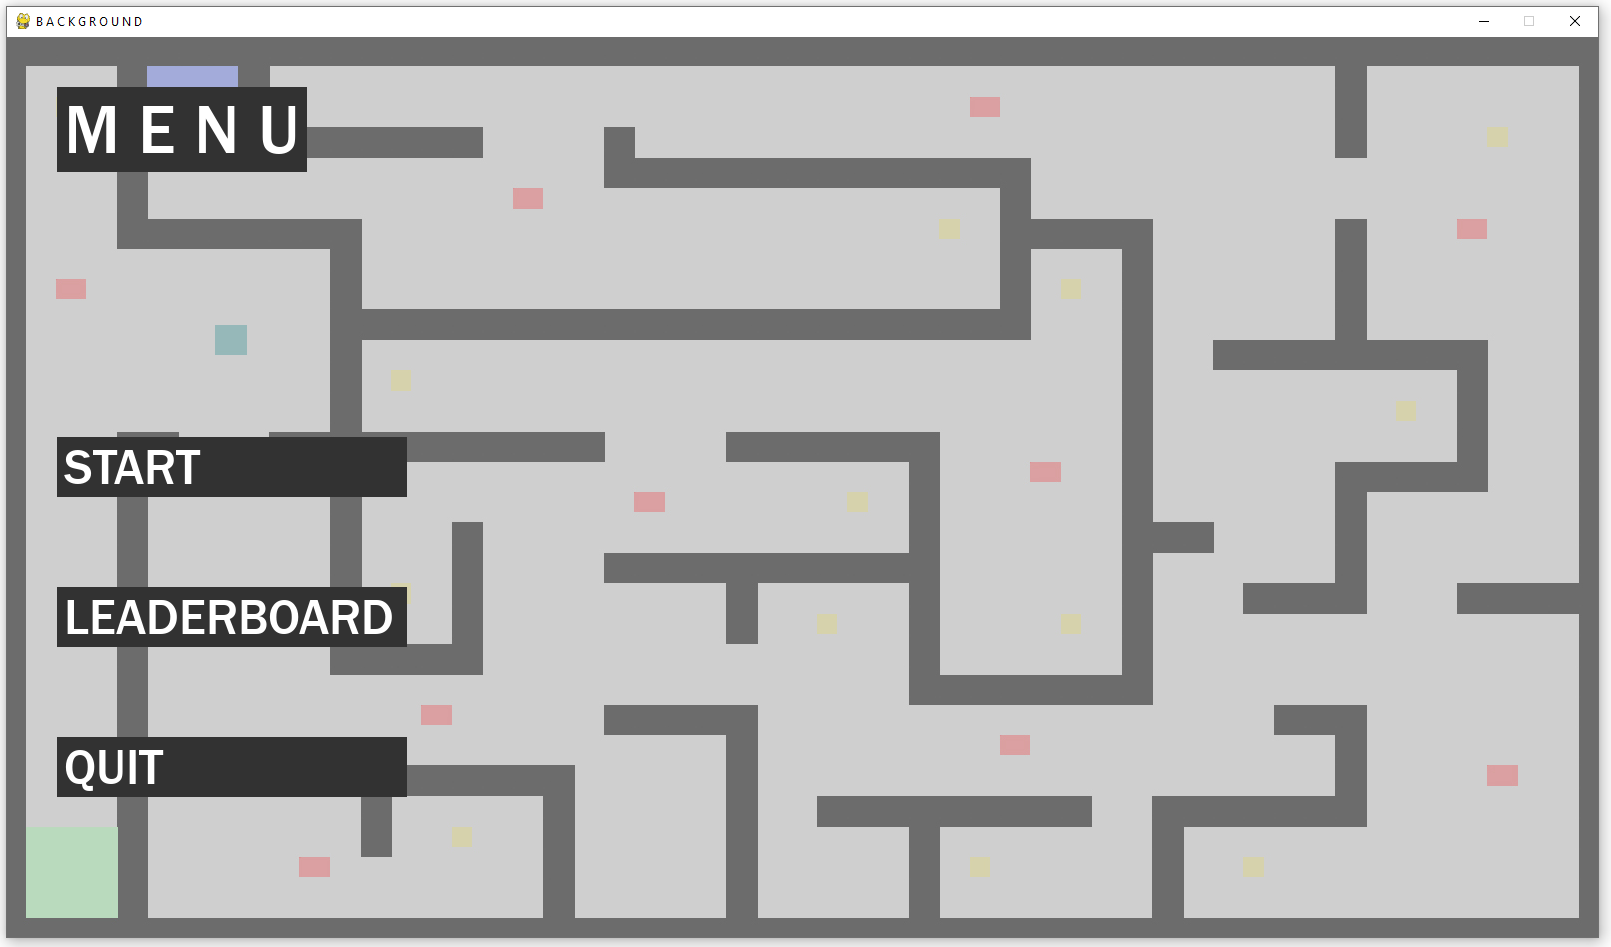
\includegraphics[width=3.5in, frame]{iteration3gameplay2.PNG}
    }
    \subfigure[Fig.b]{
    \includegraphics[width=3.5in, frame]{iteration3gameplay3.PNG}
    }
    \end{center}
    \subfigure[Fig.c]{
    \includegraphics[width=3in, frame]{iteration3gameplay4.PNG}
    }
    \subfigure[Fig.d]{
    \includegraphics[width=3in, frame]{iteration3gameplay5.PNG}
    }
    \caption{Iteration 3 Game-play}
\end{figure}

\pagebreak

\section{Post-Development Testing}
Here is the original test plan for iteration 3. I have included this here for reference. I will be conducting each of these tests and displaying the results below. I will also be discussing if each test was successful or not. I will include evidence of these tests throughout this section. 

\begin{table}[H]
    \centering
    \begin{tabular}{|c|c|c|c|}
    \hline
    \textbf{*} & \textbf{Test Description} & \textbf{Test Data} & \textbf{Expected Outcome}\\
    \hline
    1 & Game display shows menu & On click. & The menu screen is displayed \\
    & screen after start screen. & &\\
    \hline
    2 & The leader-board screen is & On click. & The program will display the\\
      & displayed on button click. & & leader-board screen constantly. \\
    \hline
    3 & The question screen is & On collision. & The question and an input box is\\
    & displayed when a coin is & & displayed to the screen. \\
    & collected. & &\\
    \hline
    4 & The question will be & On click. & The question will be skipped and\\
    & skipped if the pass button & &a point deducted from the players  \\
    & is pressed. & & score.\\
    \hline
    5 & The user will be given a & On key-press. & The program should compare the \\
    & point when the question is & & input and the data retrieved and if\\
    & answered correctly. & & they are the same, increase the score. \\
    \hline
    6 & The save score screen must & On key-press. & The users username and password\\
    & take the players username  & & will be saved to the leader-board\\
    & and save it, plus the score, & & CSV file.\\
    & to a CSV file. & & \\
    \hline
    7 & Test all quit and return & On click. & The program should quit or return\\
    & buttons. & & to the previous menu.\\
    \hline
    8 & Check alignment of text and & On event. & The text and holding rectangles \\
      & rectangles/buttons in menu & & should be aligned correctly to \\
      & screens. & & ensure the program looks professional.  \\
    \hline
    \end{tabular}
    \caption{Iteration 3 Post-Development Testing}
    \label{TestTable}
\end{table}

I have also copied the success criteria for reference throughout the testing.

\tiny
\begin{enumerate}
    \item a title screen.
    \item a menu screen. 
    \item a question screen with an input box.
    \item a leader-board screen.
    \item a 'save score' screen where the user can enter their username.
    \item an end screen.
    \item working buttons for all screens.
    \item the players score is incremented when a question is answered correctly.
    \item a wider game display, with wider levels to allow for more detail per level.
    \item the updating of existing levels to match new program size.
\end{enumerate}
\normalsize

\pagebreak

\paragraph{Test 1 (\hl{Successful} / Unsuccessful)}
Test 1 was to see if the game display displayed the menu screen after the user progresses past the first start screen. I tested this using black box testing as this test needed to be conducted in the game window. I ran this test 3 times and the outcome was the same each time; the game progressed onto the menu screen. This means that this test was successful. This successful test also proves that I have met iteration 3 success criteria point 2\footnote{Success Criteria point 2 - Implement a menu screen}.

\begin{figure}[H]
    \centering
    \includegraphics[width=4in, frame]{iteration3gameplay2.PNG}
    \caption{Menu Screen}
\end{figure}

\paragraph{Test 2 (\hl{Successful} / Unsuccessful)}
Test 2 was to see if the leader-board screen was displayed correctly when the user clicks the 'leader-board' button. I was looking for the top 10 scores to be displayed on the button click. I again used a black box approach to test this as I needed to see how the screen was displayed from an end users point of view. The leader-board displayed correctly each time I tested this feature. This test was again successful. This test proves that I have met iteration 3 success criteria point 4\footnote{Success Criteria point 4 - Implement a leader-board screen}.

\begin{figure}[H]
    \centering
    \includegraphics[width=4in, frame]{iteration3gameplay3.PNG}
    \caption{Menu Screen}
\end{figure}

\paragraph{Test 3 (\hl{Successful} / Unsuccessful)}
Test 3 was to see if the question screen was displayed when the player collects a coin. I again used black box testing to test this feature of my program. This is because this features needs to be tested in the game window, replicating how the end user will view the program. This test was successful as the question screen displayed correctly when the player collected a coin. This test also proves that I have met iteration 3 success criteria point 3\footnote{Success Criteria point 3 - Implement a question screen}.

\begin{figure}[H]
    \centering
    \includegraphics[width=4in, frame]{iteration3gameplay5.PNG}
    \caption{Menu Screen}
\end{figure}

\paragraph{Test 4 (\hl{Successful} / Unsuccessful)}
Test 4 was to see if the skip question button worked correctly. I again used a black box approach to test this feature as this is how the end user will see this feature. I tested this button 3 times and the test was mainly successful at first, with a minor change being made to improve usability. The change that I made was widening the clickable area of the button to ensure the whole rectangle was clickable. After this change was made, the button worked 100\% of the time. This test also proves that I have met iteration 3 success criteria point 7\footnote{Success Criteria point 7 - Implement working buttons}.

\paragraph{Test 5 (\hl{Successful} / Unsuccessful)}
Test 5 was to test if the users score is incremented when they answer a question correctly. I used both a white and black box approach to test this feature. I used a white box testing approach to check if the code made logical sense as to when to increment the score, and I used black box testing to check this feature was implemented correctly when using the application. This test was successful as when the question was answered correctly, the score was incremented by 1. I also added an additional feature that decreases the players score by 1 if they answer a question incorrectly. I tested this feature also, and it was successful. This also means that I have met iteration 3 success criteria point 8\footnote{Success Criteria point 8 - The players score is incremented when a question is answered correctly}.

\paragraph{Test 6 (\hl{Successful} / Unsuccessful)}
Test 6 was to test if the 'save score' screen asks the user for the players username, and then saves this along with their score to an external CSV file. I used a black box testing approach to test this as I needed to input data (the username) to see if it was saved in the correct format. I tested this 3 times with different usernames to ensure the usernames and scores saved in the correct indexes within the CSV. All three of these tests where successful, all returning the expected outcome. The program took the username of the player and stored this value in the first column of the CSV file, then saving the players score to the second column. I then checked the CSV file to see if the data had saved correctly, which it had. This proves that I have also met iteration 3 success criteria point 5\footnote{Success Criteria point 5 - Implement a 'save score' screen where the player can enter their username}.

\begin{figure}[H]
    \centering
    \includegraphics[width=4in, frame]{iteration3gameplay4.PNG}
    \caption{Menu Screen}
\end{figure}

\begin{figure}[H]
    \centering
    \includegraphics[width=3.5in, frame]{leaderboardcsv.PNG}
    \caption{Leader-Board CSV File}
\end{figure}

\paragraph{Test 7 (\hl{Successful} / Unsuccessful)}
Test 7 was to test if all the 'quit' and 'return' buttons work correctly. I used a black box approach to test this as I needed to see how the program reacted to the buttons being pressed. I tested the quit button on the menu and also the return button on the leader-board. The quit button worked correctly every time that I tested it, and returned the expected outcome. I also tested the return button on the leader-board screen; this also worked successfully each time I tested it. All of the above tests returned the expected outcome, which also means that I have met iteration 3 success criteria point 7\footnote{Success Criteria point 7 - Working buttons for all menu screens}.

\paragraph{Test 8 (\hl{Successful} / Unsuccessful)}
Test 8 was to check if the alignment of the text/buttons are all correct within the menu systems. I began with a white box testing approach as I needed to test if the text was being blited close to the rectangle. Once I was happy the text was within the co-ordinates of the rectangle, I moved to black box testing. I used black box testing to see how the text was displayed onto the rectangles/backgrounds. I had to fine tune some text and button elements to ensure they where aligned correctly, but after these tweaks the tests where successful. This also means that I have met iteration 3 success criteria point 2\footnote{Success Criteria point 2 - Implement menu screens}.

 \begin{figure}[H]
    \subfigure[Fig.a]{
    \includegraphics[width=2in, frame]{buttons1.PNG}
    }
    \subfigure[Fig.b]{
    \includegraphics[width=3.6in, frame]{buttons2.png}
    }
    \caption{Button and Text Alignment}
\end{figure}

\pagebreak

\section{Iteration 3 Evaluation}
In iteration 3, I mainly focused on implementing a fully functional system of menu screens. I chose to add this menus system now as the stakeholder asked me to in their last feedback email. I have implemented a menu screen, a leader-board screen, a save score screen, and end of game screen, and a question screen. These screens tie the game together extremely well and allow the user to navigate though the program with ease. I have also upped the game resolution from 800 x 800 to 1600 x 900. This gives the program a more complete feel and allows for bigger levels and more text to be displayed onto the screen at one time. This means that I have hit iteration 3 success criteria point 9 and 10 successfully.   
\newline
\newline
I have devised a simple system for programming any menu screens. I first start by creating a loop that displays the text and menu screen image to the screen. Then for the buttons, I display a rectangle and some text. I then check if the player has clicked within a certain area. If so, then the program will either break from the loop (i.e a quit button), or progress to a different part of the program. All of these newly implemented menu screens are fully functional with no bugs as proved in the post-development testing above. I think the implementation of a menu system has been a success in iteration 3, which meets iteration 3 success criteria point 1, 2, 3, 4, 5, 6, and 7.
\newline
\newline
Off the back of these new menu screen, I have also made the question system increment the players score every time they correctly answer a question. This feature has been tested and is fully functional as proved above within the testing. This means I have also met iteration 3 success criteria point 8. I have also added more questions and relevant answers to the question file over the course of iteration 3. This is to give the player a wider range of questions to test their knowledge on. 
\newline
\newline
Looking at features I could improve from iteration 3, I would say that the positioning and composition of all menu text/buttons needs to be scaled to fit the new game resolution. This will then allow the players to have a better experience playing the game. I will focus on improving this in iteration 4. 
\newline
\newline
Overall, I think that iteration 3 was successful as all of the features my stakeholder told me to implement at the end of iteration 2 where successfully added. I have also managed to hit every point of the success criteria that was devised at the start of the iteration, so in my opinion iteration 3 was a success. I will now present this to my stakeholder and gain feedback/next steps to inform the design decisions that I will make moving forward with iteration 4.

\pagebreak

\section{Stakeholder Conversation}
I have included the email from my stakeholder to me after their review of iteration 3. They have outlined some key points that they are happy with i.e the newly implemented menu screens. They have also provided some features that they would like to see implemented. These features will be used to influence my next steps moving forward with iteration 4. I am also looking to improve the difficulty of the questions that the users face. Moving forward with iteration 4, I would like to implement a difficulty setting to allow the users to customise this aspect of the game. I would also like to implement a health bar to add an additional challenge for the player. 


\begin{figure}[H]
    \centering
    \includegraphics[width=\linewidth, frame]{stakeholderiteration3f.PNG}
    \caption{Stakeholder Iteration 3 Feedback}
\end{figure}

\section{Next Steps}
After reviewing the feedback on iteration 3 presented to me by my stakeholder, I will now devise some goals/targets that will influence how I develop the program moving forward with iteration 4. 
\newline
\newline
I have decided that iteration 4 \textbf{must} include: 
\begin{itemize}
    \item A unique art style
    \item A login system to authenticate users
    \item A difficulty selection menu, which will change the difficulty of questions
    \item A player health bar
\end{itemize}
If there is any time left for extra development, then I will \textit{aim} to include:
\begin{itemize}
    \item 8 - 10 levels for the player to navigate
    \item 10 - 12 questions per difficulty
    \item A pause menu
    \item An options menu
    \item In-game music, which changes speed depending on health of player/if they are in a menu screen.
\end{itemize}

\pagebreak

\chapter{Iteration 4}

\begin{figure}[H]
    \centering
    \includegraphics[width=\linewidth]{iteration4title.png}
    \label{iteration2title}
\end{figure}

\pagebreak

\section{Introduction}
Over the course of iteration 4, I will be aiming to implement different features such as a difficulty system, a player health bar, and a complete graphical overhaul. I am aiming to make a fully complete solution in this iteration, so I will also be showing all of the questions and how the program is constructed from a file point of view. I will also be implementing 8 - 10 levels which are all unique in design.


\section{Iteration 4 Success Criteria}
Throughout iteration 4, I will be aiming to implement:

\begin{enumerate}
    \item A unique art style
    \item A login system
    \item Different difficulties (Easy, Medium, Hard)
    \item A player health bar
    \item A minimum of 8 unique levels
    \item A pause menu 
    \item An options menu
    \item Music that changes tempo depending on the users health
    \item A minimum of 10 questions per difficulty
    \item A full-screen mode
\end{enumerate}

\paragraph{Why?}
I have chosen to implement these features in the last stage of development as they will finish off the application nicely and make the game seem well-rounded. I have chosen to add a difficulty system to my game as I feel this feature will give the user more freedom when it comes to tailoring their revision. I have also chosen to add a player health bar to add another challenge to the game. Once the player has died 10 times, they loose. These features, along with the graphical overhaul and musical additions will complete my application and it will be ready for final robustness testing and then eventually distributed to the students for use. I will also be making the application full-screen as this is a nice quality of life addition.

\pagebreak

\section{Test Plan for Iteration 4}

\paragraph{What I Plan to Test}
in iteration 4, I will be testing to see if the newly implemented difficulty and player health features are functioning correctly. I will also be testing to ensure the new graphical changes work correctly as I will be changing most of the textures. 

\begin{table}[H]
    \centering
    \begin{tabular}{|c|c|c|c|}
    \hline
    \textbf{*} & \textbf{Test Description} & \textbf{Test Data} & \textbf{Expected Outcome}\\
    \hline
    1 & All updated textures must & On start. & The textures are displayed \\
    & be displayed correctly. & & correctly, including in menus.\\
    \hline
    2 & The login system must  & On input. & The program will progress\\
      & correctly authenticate users. & & if a found username is entered. \\
    \hline
    3 & The player will lose HP  & On collision. & The players health bar is\\
    & when collided with an enemy & & decreased by the correct amount. \\
    \hline
    4 & The correct music will play & On collision. & The music will change tempo\\
    & depending on the players & & depending on the players health.  \\
    & health. & & \\
    \hline
    5 & The game will pause when & On event. & The program should display the \\
    & the pause button is clicked & & pause menu.\\
    \hline
    6 & The program will display & On key-press. & The program should display\\
    & the options menu when clicked. & & the options menu.\\
    \hline
    7 & Test if the full-screen works & On start. & The program should be in\\
    & correctly. & & full-screen mode on start.\\
    \hline
    8 & Check if selecting different & On event. & The questions will change \\
      & difficulties changes & & depending on the difficulty selected. \\
      & the questions. & & \\
    \hline
    \end{tabular}
    \caption{Iteration 4 Pre-Development Testing Plan}
    \label{TestTable}
\end{table}

\pagebreak

\section{Code Development}

\subsection{The Player Health System}
To add a health bar for the player, I first started by creating a 'health' variable and setting it to 200. I have chosen 200 because the player health bar size will be dictated off of this number, and I want it to be large enough to look in place on the display.

\begin{Verbatim}[numbers=left, frame=single] 
# Sets players health to 200
health = 200
\end{Verbatim}

I then implemented two rectangles, one red and the other green. I have used these rectangles to display the players health in a health bar fashion. Every time the player collides with and enemy, the green rectangle is decreased by 20 pixels on the x plane.

\small

\begin{Verbatim}[numbers=left, frame=single] 
# Checks for collision
if pygame.sprite.spritecollide(p1 ,enemy_group,False):
   # Deducts 20 from the players health if collided
   health -= 20
   if health == 0:
       # Handles lose and quit screens 
       while True:                                                             
           for event in pygame.event.get():
               if event.type == pygame.MOUSEBUTTONDOWN:
                   mouse = pygame.mouse.get_pos()
                   if event.type == pygame.MOUSEBUTTONDOWN:
                       if 0 <= mouse[0] <= 1920 and 0 <= mouse[1] <= 1080:
                           lb.writeScores(score,gameDisplay,fps,username)
                           m.endScreen(gameDisplay,fps)
                           running = False
                           break
\end{Verbatim}

\normalsize

This section of code checks if the player has collided with an enemy. If so, then it will deduct 20 from the players health. It will also check if the players health is 0. If it is, then the program will display the you have lost screen, the save score screen, and then quit the program. 

The code below is used to display the players health and health bar to the game display. I have done this as they player needs to see how much health the have left when playing the game.

\begin{Verbatim}[numbers=left, frame=single]
health_text = ("HEALTH: "+str(health))
\end{Verbatim}

\begin{Verbatim}[numbers=left, frame=single]
pygame.draw.rect(gameDisplay, red, [15,1000,200,50])
pygame.draw.rect(gameDisplay, green, [15,1000,health,50])
\end{Verbatim}

\section{Difficulties}
I have implemented three difficulties into my game. These difficulties are easy, normal, and hard. Depending on the difficulty the player selects, the questions will change i.e if hard is selected the program will read all questions from the 'hard questions' CSV file. I have created a difficulty selection screen that will change where the questions are chosen from. I will display this below. I have programmed it this way as this was the most efficient method of implementing different difficulties. 

\begin{Verbatim}[numbers=left, frame=single]
if event.type == pygame.MOUSEBUTTONDOWN:
    mouse = pygame.mouse.get_pos()
    if 0 <= mouse[0] <= 1920 and 0 <= mouse[1] <= 1080:
        menu1 = False
        play = m.subMenu(gameDisplay,fps)
        username = m.login(
                 score,text,color,color_active,color_inactive,
                 active,gameDisplay,fps)
        qIndex, aIndex = m.difficulty(aIndex,qIndex,gameDisplay,fps)
        if qIndex == 0:
            diff_text = "DIFFICULTY: Easy"
        elif qIndex == 1:
            diff_text = "DIFFICULTY: Normal"
        else:
            diff_text = "DIFFICULTY: Hard"
\end{Verbatim}

This section of code uses functions from libraries that I have created for my game. I will discuss and display these libraries later in the development stage. I have also move all the questions to one CSV file, and all of the answers to a single CSV file. The program will index this file depending on the difficulty selected. This helps to keep things tidy and also allows for easier maintenance
in the future. 

I have also included a screen shot of the question and answer CSV files. If the user selects easy, the programs index value will be 0, if they select medium it will be 1, and so on.

 \begin{figure}[H]
    \subfigure[Fig.a]{
    \includegraphics[width=3.75in, frame]{questions csv.PNG}
    }
    \subfigure[Fig.b]{
    \includegraphics[width=2in, frame]{answers csv.PNG}
    }
    \caption{Question and Answer CSV Files}
\end{figure}

\section{The Login System}
I have implemented a login system to my game. I have done this because it will only allow authenticated users from playing the game. This could be used by the teachers to hand out logins to the class, that way no students will enter a peers name and interfere with their score. I will be displaying and explaining the code for this login system below.

\scriptsize

\begin{Verbatim}[numbers=left, frame=single]
def login(score,text,color,color_active,color_inactive,active,gameDisplay,fps):
    text = ""
    active = False
    login = True
    try_again = False
    found = False
    usernames = open("csv/usernames.csv")
    check_usernames = csv.reader(usernames)
    while login is True:
        for event in pygame.event.get():
            if event.type == pygame.MOUSEBUTTONDOWN:
                mouse = pygame.mouse.get_pos()
                if event.type == pygame.MOUSEBUTTONDOWN:
                    if 0 <= mouse[0] <= 100 and 0 <= mouse[1] <= 100:
                        login = False
                        break
                if input_box.collidepoint(event.pos):
                    active = not active
                else:
                    active = False
                color = color_active if active else color_inactive
            if event.type == pygame.KEYDOWN:
                if active is True and found is False:
                    if event.key == pygame.K_RETURN:
                        for x in check_usernames:
                            if text.lower() == x[0].lower():
                                print("F")
                                found = True
                                return text
                            
                        if found is False:
                            print("NF")
                            text = ""
                            try_again = True
                            usernames = open("csv/usernames.csv")
                            check_usernames = csv.reader(usernames)
                        
                    elif event.key == pygame.K_BACKSPACE:
                        text = text[:-1]
                    else:
                        text += event.unicode
            break
        
        gameDisplay.blit(backG, (0,0))
        txt_surface = font_titleL.render(text, True, color)                                        
        width = max(1000, txt_surface.get_width()+10)                                       
        input_box.w = width
        gameDisplay.blit(txt_surface, (input_box.x+10, input_box.y+5))                      
        pygame.draw.rect(gameDisplay, color, input_box, 3)
        menu_text9 = font_titleLarge.render("ENTER USERNAME",True,white)
        gameDisplay.blit(menu_text9, (50,30))
        menu_text10 = font_title.render("ENTER YOUR USERNAME",True,white)
        gameDisplay.blit(menu_text10, (640,630))
        if try_again == True:
            menu_text11 = font.render("USERNAME NOT FOUND, TRY AGAIN",True,white)
            gameDisplay.blit(menu_text11, (300,300))
        text = text
\end{Verbatim}

\normalsize

For the login system, I have created a new screen in which the user can input their username. The program will then check to see if that username is found in a list stored in an external CSV file. If the user enters and input that is not listed in this usernames file, then the program will ask the user to try again. I will include an example of the usernames CSV below.

\begin{figure}[H]
    \centering
    \includegraphics[width=\linewidth,frame]{usernames csv.PNG}
    \caption{Usernames CSV File}
\end{figure}

\pagebreak

\section{The Pause Menu}
I have added pause menu so the user can quit whilst playing the game. I have also added an options button so that an options menu can be implemented in the future. I will include a code snippet below of this pause menu. I have writ en this function in the menu library I have created for my program.

\small

\begin{Verbatim}[numbers=left, frame=single]
def pauseM(gameDisplay,fps):
    while True:
        for event in pygame.event.get():
            if event.type == pygame.QUIT:
                pygame.quit()
                quit()
            if event.type == pygame.MOUSEBUTTONDOWN:
                mouse = pygame.mouse.get_pos()
                if 840 <= mouse[0] <= 1060 and 390 <= mouse[1] <= 470:
                    return "play"
                if 840 <= mouse[0] <= 1060 and 590 <= mouse[1] <= 670:
                    return "option"
                if 840 <= mouse[0] <= 1060 and 790 <= mouse[1] <= 870:
                    pygame.quit()
                    quit()

        gameDisplay.blit(backG, (0,0))  
        menu_text1 = font_titleLarge.render("PAUSE", True, white)
        gameDisplay.blit(menu_text1, (50,50))
        pygame.draw.rect(gameDisplay, darkGrey, [850, 400, 220 , 60])
        pygame.draw.rect(gameDisplay, darkGrey, [850, 600, 220 , 60])
        pygame.draw.rect(gameDisplay, darkGrey, [850, 800, 220 , 60])
        menu_text2 = font_sub.render("CONTINUE", True, white)
        gameDisplay.blit(menu_text2, (865,415))
        menu_text3 = font_sub.render("OPTIONS", True, white)
        gameDisplay.blit(menu_text3, (875,615))
        menu_text4 = font_sub.render("QUIT", True, white)
        gameDisplay.blit(menu_text4, (910,815))
        pygame.display.update()                                                                     
        clock.tick(fps)
\end{Verbatim}

\normalsize

I have used the menu screen template from iteration 3 to add the pause menu into the game. I have added this feature to allow the player to exit or view the options menu whilst mid-way through the game. I have chosen to put this in a function within the menu library as this will make it easy for future changes to be made as all the menu screens are grouped in one library. 

\section{File Structure}
As I have been developing my project, I have built a well-organised file structure that includes folders for all images, CSV files, sound files and documentation. I have also separated my program into a main file and 3 additional libraries. This has helped me organise my project when it has become substantial. I will display this file structure below.

\begin{figure}[H]
    \centering
    \includegraphics[width=\linewidth,frame]{files.PNG}
    \caption{Folder Structure}
\end{figure}

\begin{figure}[H]
    \centering
    \includegraphics[width=\linewidth,frame]{files2.PNG}
    \caption{Folder Structure}
\end{figure}


\pagebreak

\section{Screenshots of Game-Play}
I have included some screenshots of game-play below. The screenshots are of the newly implemented graphics, login screen, health bar, and pause menu. The application is now to a standard in which it can be given to my stakeholder for distribution, after the final stage of testing. My login system also has elements of validation which is shown further along in this document.

 \begin{figure}[H]
    \begin{center}
    \subfigure[Fig.a]{
    \includegraphics[width=3.4in, frame]{it43.PNG}
    }
    \subfigure[Fig.b]{
    \includegraphics[width=3.4in, frame]{it44.PNG}
    }
    \end{center}
    \subfigure[Fig.c]{
    \includegraphics[width=2.7in, frame]{it41.PNG}
    }
    \subfigure[Fig.d]{
    \includegraphics[width=3in, frame]{it42.PNG}
    }
    \caption{Iteration 4 Game-play}
\end{figure}

\section{Post-Development Testing}
Here is the original test plan for iteration 4. I have copied this down for reference when conducting the post-development testing. I will refer back to this table when testing an I will also be evaluating whether each test is successful or not.

\begin{table}[H]
    \centering
    \begin{tabular}{|c|c|c|c|}
    \hline
    \textbf{*} & \textbf{Test Description} & \textbf{Test Data} & \textbf{Expected Outcome}\\
    \hline
    1 & All updated textures must & On start. & The textures are displayed \\
    & be displayed correctly. & & correctly, including in menus.\\
    \hline
    2 & The login system must  & On input. & The program will progress\\
      & correctly authenticate users. & & if a found username is entered. \\
    \hline
    3 & The player will lose HP  & On collision. & The players health bar is\\
    & when collided with an enemy & & decreased by the correct amount. \\
    \hline
    4 & The correct music will play & On collision. & The music will change tempo\\
    & depending on the players & & depending on the players health.  \\
    & health. & & \\
    \hline
    5 & The game will pause when & On event. & The program should display the \\
    & the pause button is clicked & & pause menu.\\
    \hline
    6 & The program will display & On key-press. & The program should display\\
    & the options menu when clicked. & & the options menu.\\
    \hline
    7 & Test if the full-screen works & On start. & The program should be in\\
    & correctly. & & full-screen mode on start.\\
    \hline
    8 & Check if selecting different & On event. & The questions will change \\
      & difficulties changes & & depending on the difficulty selected. \\
      & the questions. & & \\
    \hline
    \end{tabular}
    \caption{Iteration 4 Post-Development Testing Plan}
    \label{TestTable}
\end{table}

I have also copied the success criteria for reference throughout the testing. 

\small

\begin{enumerate}
    \item A unique art style
    \item A login system
    \item Different difficulties (Easy, Medium, Hard)
    \item A player health bar
    \item A minimum of 8 unique levels
    \item A pause menu 
    \item An options menu
    \item Music that changes tempo depending on the users health
    \item A minimum of 10 questions per difficulty
    \item A full-screen mode
\end{enumerate}

\normalsize 

\paragraph{Test 1 (\hl{Successful} / Unsuccessful)}
Test 1 was to see if all the updated textures where displayed correctly to the screen. I used a black box approach to test this problem as I had to see the game running to know the outcome. This test was successful as all of the newly drawn textures where displayed on each tile correctly. This is done by the program as it will scale each texture to fit the size of the tile. There is evidence of this below. This test also proves I have met iteration 4 success criteria point 1\footnote{Success Criteria Point 1 - Implement a unique art style.}. 

\begin{figure}[H]
    \centering
    \includegraphics[width=4in,frame]{it43.PNG}
    \caption{Updated Textures}
\end{figure}

\paragraph{Test 2 (\hl{Successful} / Unsuccessful)}
Test 2 was to see if the login system would correctly authenticate users. I used a combination of white and black box testing to test this as looking through the code help me find logical errors, and the game window testing helped me find what exactly the errors where. There was one error in which if a username is entered incorrectly, a correct one couldn't be entered after. This bug is now fixed and the login system is now fully functional. I will evidence this below. This test also proves that I have met iteration 4 success criteria point 2\footnote{Success Criteria Point 2 - Implement a login system.}.

\begin{figure}[H]
    \centering
    \includegraphics[width=3in,frame]{it41.PNG}
    \caption{Updated Textures}
\end{figure}

\paragraph{Test 3 (\hl{Successful} / Unsuccessful)}
Test 3 was to see if the player loses HP (health points) when they collide with an enemy tile. I used a black box approach to test this feature as it had to be conducted inside of the game window. I started by logging in, selecting the normal difficulty and running into an enemy tile. The test was successful as the players health bar decreased by 20 HP every time they collided with an enemy. I will evidence this below. This test also proves that I have met iteration 4 success criteria point 4\footnote{Success Criteria Point 4 - Implement a working player health bar.}.

\begin{figure}[H]
    \centering
    \includegraphics[width=\linewidth,frame]{test 4.png}
    \caption{Player Health Bar}
\end{figure}

\paragraph{Test 4 (Successful / \hl{Unsuccessful})}
Test 4 was to see if the music changed depending on the players health level. This test was unsuccessful as I did not have enough development time left in this iteration to implement this feature. This could be a feature to add in the future and send to the stakeholder as an update. This also means that I have failed to meet iteration 4 success criteria point 8\footnote{Success Criteria Point 8 - Implement different music depending on the players health.}.

\paragraph{Test 5 (\hl{Successful} / Unsuccessful)}
Test 5 was to see if the game would pause when the on-screen pause button was clicked. I again used a black box approach to conduct this test as the pause button needs to be physically clicked from within the game window. This test was successful and the program paused and also displayed the pause menu when clicked. I will evidence this below. This proves that I have also met iteration 4 success criteria point 6\footnote{Success Criteria Point 6 - Implement a pause menu.}. 

\begin{figure}[H]
    \centering
    \includegraphics[width=3.5in,frame]{pauseM.PNG}
    \caption{Pause Menu}
\end{figure}

\paragraph{Test 6 (Successful / \hl{Unsuccessful)}}
Test 6 was to see if the program displayed an options menu when the options button was clicked from within the pause menu. This test was unsuccessful as I didn't have enough left time in development to implement this feature. I have added the button which prints "Options" to the console, I just haven't added an options screen as I didn't consider this feature to be of a high priority. This also means that I have failed to meet iteration 4 success criteria point 7\footnote{Success Criteria Point 7 - Implement an options menu}.

\paragraph{Test 7 (\hl{Successful} / Unsuccessful)}
Test 7 was to see if the game ran okay in full-screen mode. I again used black box testing as I needed to see what the game window looked like in full-screen mode. After re-aligning some of the menu buttons/text, the test was successful and had no issues with implementation. I will evidence this below. This test also means that I have met iteration 4 success criteria point 10\footnote{Success Criteria Point 10 - Implement a full-screen resolution feature.}.

\begin{figure}[H]
    \centering
    \includegraphics[width=2.5in,frame]{fullscreen.PNG}
    \caption{Full-Screen Resolution}
\end{figure}

\paragraph{Test 8 (\hl{Successful} / Unsuccessful)}
Test 8 was to see if changing the difficulty selected changed the content of the questions in which the user where asked. I used a combination of a black and white box approach to test if the feature was working correctly. I firstly started by checking the code to see if depending on the difficulty selected, would the index value of the CSV file change. The code was in working order so then I tested this though the game window via playing the game. This test was successful as depending on the difficulty you chose, you will receive different questions when collecting a coin. I will evidence this below. This also means that I have met iteration 4 success criteria point 3\footnote{Success Criteria Point 3 - Implement different difficulties.}.

\begin{figure}[H]
    \centering
    \includegraphics[width=2.5in,frame]{answers csv.PNG}
    \caption{Different Difficulty Questions}
\end{figure}


\pagebreak

\section{Iteration 4 Evaluation}
Looking back at iteration 4, the features I chose to implement worked successfully however I didn't implement all intended features due to a time constraint. I just didn't think these features would be necessary or effect the quality of the final outcome in any way. This iteration I mainly focused on implementing a player health bar, a login system, a difficulty system and a graphical overhaul. I think iteration 4 was successful as I have implemented the listed featured with no bugs/flaws still remaining. I have met 8 out of the 10 success criteria points, and the points in which I have met have been implemented at a high standard. 
\newline
\newline
Moving forward with this project, I could come back and implement the features I have missed in this iteration as an 'update' and release it to my stakeholder. This will keep the game feeling fresh and will allow for the students to be continuously engaged with the program, as new content will be released.
\newline
\newline
Overall, I think iteration 4 was successful in some aspects, but not successful in implementing all the desired features of the stakeholder. I think that the program as a whole is ready for distribution by my stakeholder, so that students can play the game and revise just in time for their GCSE exams. I will now be sending this final version to my stakeholder for review and for them to give me any feedback for future updates.

\section{Stakeholder Conversation}
I have presented the final version of my application to my stakeholder and this is what they had to say.

\begin{figure}[H]
    \centering
    \includegraphics[width=\linewidth,frame]{sfeedbackit4.PNG}
    \caption{Stakeholder Iteration 4 Feedback}
\end{figure}

\chapter{Final Testing and Evaluation}

\section{Final Testing}
Over the course of the final testing, I will be testing the robustness and usability of my program and how it will handle when given to the user. I will be explaining each test, conducting the test, and then writing up my findings. 

\paragraph{Test 1 - Can the player quit at any point?}
Yes - The player can quit the game at any point. This is either through quit buttons that have been programmed and placed onto the screen, or through the red 'X' button in the top right hand corner of the game window. 

\paragraph{Test 2 - Can CSV's be updated and changes recognised?}
Yes - When you change a value in one of the external CSV files, the next time the program is run it will use the newly updated data set. I.e if you add a username, the next time the program is used, that username will be recognised.

\paragraph{Test 3 - Do all collisions work and can they be exploited?}
I have been testing the game for over an hour trying to exploit all walls/collisions and can not find a single way to do so. This means that levels can't be skipped and the player must play the game how it was intended to be played when being developed. 

\paragraph{Test 4 - Is the game easy to use?}
I would consider this solution easy to use as their are multiple menu screens, which all use a clear, legible, large font. The program is also very self explanatory as their is only one way to the exit. The player can see this and has a natural instinct to travel in that direction. They also are inclined to collect the coins and avoid enemies as this is what is traditionally done in video games. The HUD is also self-explanatory and provides the user with some helpful information.

\section{Maintenance Guide}
I have created a maintenance guide for the stakeholder so that they can maintain/edit the program however they like. Here is a screenshot of the Maintenance Guide. This guide is just a brief reminder of how to change textures/edit levels/edit CSV files as I have already explained to the stakeholder in-depth about how to do these things.

\begin{figure}[H]
    \centering
    \includegraphics[width=\linewidth,frame]{Mguide.PNG}
    \caption{Maintenance Guide}
\end{figure}

\pagebreak

\footnotesize

\section{Final Evaluation}
Looking back on the project, it was successful overall with all of the implemented features working as intended. I will be evaluating my program as a whole and identifying Strong/weak points of my application.

\paragraph{Iteration 1}
In iteration 1, I set out to just create the basics of a game i.e a game window and moving sprite. I had got these features working but that was all. I met all of the success criteria points that where devised for iteration 1. The post-development testing also shows this as each test that I conducted was successful. If I where to re-do iteration 1, I would add some basic collision features to stop the player leaving the walls of the level. I implemented the 'x' button functionality in this iteration to improve the usability of the program. This is so the program could be closed at any time. I consider this iteration a success as I have met all the points in the success criteria that was devised for this iteration. I will copy this success criteria below for reference. 

\paragraph{Iteration 1 Success Criteria}
\begin{enumerate}
    \item run on a school computer at 60 FPS.
    \item run in a separate game window from the python IDLE shell.
    \item display a working player model with basic collisions.
    \item display a background to the game window.
    \item close when the 'X' button is pressed at any time.
    \item all files saved into a single project folder.
    \item include basic platform for development i.e creation of classes, ready for iteration 2.
\end{enumerate}

\paragraph{Iteration 2}
Moving on to iteration 2 where the game started to gain enough features to become playable. I aimed to implement 8 features in iteration 2, and did so successfully. This iteration is where I added features such as the level system and basic collisions. The post development testing shows that this iteration was successful as each test was completed with no errors. This is mainly because I have been debugging as I have developed the code. I consider this iteration to also be successful as I have met every pointy of the success criteria that was devised for iteration 2. I will copy this success criteria below for reference.


\paragraph{Iteration 2 Success Criteria}
\begin{enumerate}
    \item working collisions between the player and level environment.
    \item a score counter, which is incremented every time a player collides with a coin, onto the screen at all times.
    \item a timer for each level.
    \item basic conditional text screens i.e. when the player has ran out of time or completed the game.
    \item sound effects for collisions such as with an enemy, with a coin, or the exit gate.
    \item a wide range of custom levels, with all level data stored in a 'levels' folder.
    \item a grid-like level layout, with each block-type having a unique and identifiable texture.
    \item the player is reset to the start when they collide with an enemy.
\end{enumerate}

\pagebreak

\footnotesize

\paragraph{Iteration 3}
Iteration 3 was where the most progress was made in terms of development. Over the course of this iteration I managed to implement multiple menu screens which can be navigated around, a question screen to ask the user for answers to various different questions, a leader-board which will display data stored on an external CSV file, and also some small graphical changes. I think that this iteration was successful as I managed to meet every point of the success criteria for this iteration successfully. I will copy this success criteria below for reference.

\paragraph{Iteration 3 Success Criteria}
\begin{enumerate}
    \item a title screen.
    \item a menu screen. 
    \item a question screen with an input box.
    \item a leader-board screen.
    \item a 'save score' screen where the user can enter their username.
    \item an end screen.
    \item working buttons for all screens.
    \item the players score is incremented when a question is answered correctly.
    \item a wider game display, with wider levels to allow for more detail per level.
    \item the updating of existing levels to match new program size.
\end{enumerate}

\paragraph{Iteration 4}
The final iteration, iteration 4, was where most of the quality of life and final features where implemented. I implemented a player health bar, a difficulty system, a player HUD (heads up display), and completely changed all of the textures/menu screens/fonts of the game. This is to make the solution feel high-quality and rounded, so that it can be sent to the stakeholder for distribution. I would again consider this a successful iteration as I have met 8 out of the 10 points set in the iteration success criteria. The only two points that I failed to meet in this iteration where the implementation of additional music and an options menu. I chose to fixate on the other features more and ensure they where implemented to the highest standard instead of waste development time on these features. I can implement these features at a later date and release them as updates for the students to experiment with. I will copy this success criteria below for reference.

\paragraph{Iteration 4 Success Criteria}
\begin{enumerate}
    \item A unique art style
    \item A login system
    \item Different difficulties (Easy, Medium, Hard)
    \item A player health bar
    \item A minimum of 8 unique levels
    \item A pause menu 
    \item An options menu
    \item Music that changes tempo depending on the users health
    \item A minimum of 10 questions per difficulty
    \item A full-screen mode
\end{enumerate}

\pagebreak

\paragraph{Overall Success Criteria}
Looking back at the original overall success criteria, I will be evaluating the program as a whole compared to this criteria. I will copy each point down and then discuss how well I have met each section.

\begin{enumerate}
    \item \textbf{Always include a fully functioning exit game button}
\end{enumerate}

I have met this success criteria point throughout all of my iterations.

\begin{enumerate}
    \item[2.] \textbf{Include a scoreboard with all of the players scores displayed on it}
\end{enumerate}

I have met this success criteria point fully as my final program has a fully-functional leader-board system.

\begin{enumerate}
    \item[3.] \textbf{Include a multi room game}
\end{enumerate}

I have meth this success criteria point as my final solution has multiple levels for the user to navigate/explore.

\begin{enumerate}
    \item[4.] \textbf{Include characters that the player can interact with}
\end{enumerate}

I have failed to meet this success criteria point as I have chosen to add coins which ask questions on collection instead of implementing characters in which the player can interact with. This feature could be revisited in a future update.

\begin{enumerate}
    \item[5.] \textbf{Include objects that the player can interact with}
\end{enumerate}

I have met this success criteria point successfully as I have implemented collectable coins and enemies in which the player can interact with. This is shown in the development further above in this document.

\begin{enumerate}
    \item[6.] \textbf{Work on all computer systems within the school}
\end{enumerate}

I have met this success criteria point successfully as the computer on which the game was developed was a school machine. This means that the program will have no issue running on these school computers.

\begin{enumerate}
    \item[7.] \textbf{Convey information in an educational and easy to understand manner}
\end{enumerate}

I have met this success criteria point as my stakeholder for this project has expressed how well they think the question system will engage the users. I have also gained feedback from students and they have said that this style of questioning would appeal to them.

\begin{enumerate}
    \item[8.] \textbf{Working character animations}
\end{enumerate}

I have not met this success criteria point as I have chosen to go with a rectangular player model instead. In a future update, I can implement these character animations with an updated player model.

\begin{enumerate}
    \item[9.] \textbf{Working physics for player characters}
\end{enumerate}

I have met this success criteria point successfully as I have implemented working collisions between the player and the world/collectables/enemies. 

\begin{enumerate}
    \item[10.] \textbf{Working score counter visible to the player when playing the game}
\end{enumerate}

I have met this success criteria point successfully as I have managed to implement a working score counter throughout my program.

\pagebreak
\paragraph{Limitations}
Throughout the project I have encountered some limitations when developing my program. The first limitation I encountered when developing the code was my physical ability. My programming ability held me back and I had to allow for longer than anticipated for development time. I overcame this limitation by practicing programming skills and working hard to improve myself as a programmer. I also encountered a time-scale limitation towards the end of my project. In iteration 4, I struggled to find the time to implement all of the features that where aimed to achieve at the start i.e more music and more levels. This limitation has had an effect on my final program and will be something to consider more heavily at the start of the project next time.

\paragraph{Final Comments}
Overall, I am extremely pleased with my solution to my stakeholders original problem. I think that 'Background' is a fun yet educational game which will cement the key knowledge and definitions of computer science into the brains of any of the students that may use it in the future. Moving forward with any future programs I choose to create, I would do a few thing differently. I would like to allocate more time for development so that my maximum potential can be shown through the development of an epic project such as a 3D game or open world adventure game etc. I would also like to do more research into how students learn so that I can use this to influence design decisions when it comes to the educational aspect of my solution.
\newline
\newline
Thank you for taking the time to read this report, I hope you have enjoyed the work I have produced.
\newline
\newline
\textit{Tom.}

\normalsize











\label{mylastpage}

\appendix

\chapter{Code}
\label{appendix}
\pagenumbering{roman}
\setcounter{page}{13}

\textbf{Leaderbaord.py}
\tiny
\begin{Verbatim}[numbers=left, frame=single]
import pygame
import csv

pygame.init()                                                                               
clock = pygame.time.Clock()

font = pygame.font.Font("fonts/Eight-Bit Madness.ttf", 20)
font_sub = pygame.font.Font("fonts/Eight-Bit Madness.ttf", 50)
font_title = pygame.font.Font("fonts/Eight-Bit Madness.ttf", 70)
font_titleL = pygame.font.Font("fonts/Eight-Bit Madness.ttf", 100)
font_titleLarge = pygame.font.Font("fonts/Eight-Bit Madness.ttf", 150)

backG = pygame.image.load("img/backgrounds/backgroundLarge.png")

nextB = pygame.image.load("img/buttons/nextB.png")

input_box = pygame.Rect(460, 700, 1000, 64)                                                  

black = (0,0,0)
darkGrey = (50,50,50)
white = (255,255,255)

def printLeaderboard(gameDisplay,fps):
    leaderboardArray = []
    leaderboard = open("csv/leaderboard.csv")
    check = csv.reader(leaderboard)
    for x in check:
        leaderboardArray.append(x[0])
        leaderboardArray.append(x[1])

    while True:
        for event in pygame.event.get():
            if event.type == pygame.QUIT:
                pygame.quit()
                quit()

            if event.type == pygame.MOUSEBUTTONDOWN:
                mouse = pygame.mouse.get_pos()
                if 1280 <= mouse[0] <= 1510 and 790 <= mouse[1] <= 870:
                    return False
                
        d = {}
        for x in range(0,20,2):
            d["string{0}".format(x)] = leaderboardArray[x]
        d2 = {}
        for x in range(1,20,2):
            d2["string{0}".format(x)] = leaderboardArray[x]
                        
        gameDisplay.blit(backG, (0,0))
        lb1_text = font_title.render(d["string0"],True,white)
        lb2_text = font_title.render(d["string2"],True,white)
        lb3_text = font_title.render(d["string4"],True,white)
        lb4_text = font_title.render(d["string6"],True,white)
        lb5_text = font_title.render(d["string8"],True,white)
        lb6_text = font_title.render(d["string10"],True,white)
        lb7_text = font_title.render(d["string12"],True,white)
        lb8_text = font_title.render(d["string14"],True,white)
        lb9_text = font_title.render(d["string16"],True,white)
        lb10_text = font_title.render(d["string18"],True,white)

        lb11_text = font_title.render(d2["string1"],True,white)
        lb12_text = font_title.render(d2["string3"],True,white)
        lb13_text = font_title.render(d2["string5"],True,white)
        lb14_text = font_title.render(d2["string7"],True,white)
        lb15_text = font_title.render(d2["string9"],True,white)
        lb16_text = font_title.render(d2["string11"],True,white)
        lb17_text = font_title.render(d2["string13"],True,white)
        lb18_text = font_title.render(d2["string15"],True,white)
        lb19_text = font_title.render(d2["string17"],True,white)
        lb20_text = font_title.render(d2["string19"],True,white)

        gameDisplay.blit(lb1_text, (100,200))
        gameDisplay.blit(lb2_text, (100,275))
        gameDisplay.blit(lb3_text, (100,350))
        gameDisplay.blit(lb4_text, (100,425))
        gameDisplay.blit(lb5_text, (100,500))
        gameDisplay.blit(lb6_text, (100,575))
        gameDisplay.blit(lb7_text, (100,650))
        gameDisplay.blit(lb8_text, (100,725))
        gameDisplay.blit(lb9_text, (100,800))
        gameDisplay.blit(lb10_text, (100,875))

        gameDisplay.blit(lb11_text, (800,200))
        gameDisplay.blit(lb12_text, (800,275))
        gameDisplay.blit(lb13_text, (800,350))
        gameDisplay.blit(lb14_text, (800,425))
        gameDisplay.blit(lb15_text, (800,500))
        gameDisplay.blit(lb16_text, (800,575))
        gameDisplay.blit(lb17_text, (800,650))
        gameDisplay.blit(lb18_text, (800,725))
        gameDisplay.blit(lb19_text, (800,800))
        gameDisplay.blit(lb20_text, (800,875))
    
        menu_text7 = font_title.render("Return", True, white)
        pygame.draw.rect(gameDisplay, darkGrey, [1290, 800, 220 , 60])
        gameDisplay.blit(menu_text7, (1304,811))
        menu_text8 = font_titleLarge.render("LEADERBOARD",True,white)
        gameDisplay.blit(menu_text8, (50,30))
        pygame.display.update()                                                                 
        clock.tick(fps)

def writeScores(score,gameDisplay,fps,username):
    writeScore = True
    while writeScore is True:
        for event in pygame.event.get():
            if event.type == pygame.MOUSEBUTTONDOWN:
                mouse = pygame.mouse.get_pos()
                if event.type == pygame.MOUSEBUTTONDOWN:
                    if 0 <= mouse[0] <= 1920 and 0 <= mouse[1] <= 1080:
                        writeScore = False
                        break
        
        gameDisplay.blit(backG, (0,0))
        menu_text9 = font_titleLarge.render(" Your score has been saved",True,white)
        gameDisplay.blit(menu_text9, (50,50))
        gameDisplay.blit(nextB, (1600,800))
        pygame.display.update()                                                                 
        clock.tick(fps)
    
    leaderboard = open("csv/leaderboard.csv", "at")
    leaderboard.write(username+","+str(score)+"\n")
    leaderboard.close()
\end{Verbatim}
\normalsize

\pagebreak

\textbf{Menu.py}
\tiny
\begin{Verbatim}[numbers=left, frame=single]
import pygame
import leaderboard as lb
import csv

pygame.init()                                                                               
clock = pygame.time.Clock()

font = pygame.font.Font("fonts/Eight-Bit Madness.ttf", 20)
font_sub = pygame.font.Font("fonts/Eight-Bit Madness.ttf", 50)
font_title = pygame.font.Font("fonts/Eight-Bit Madness.ttf", 70)
font_titleL = pygame.font.Font("fonts/Eight-Bit Madness.ttf", 100)
font_titleLarge = pygame.font.Font("fonts/Eight-Bit Madness.ttf", 150)

input_box = pygame.Rect(460, 700, 1000, 64)                                                  

backG = pygame.image.load("img/backgrounds/backgroundLarge.png")

black = (0,0,0)
darkGrey = (50,50,50)
white = (255,255,255)

def subMenu(gameDisplay,fps):
    while True:
        for event in pygame.event.get():
            if event.type == pygame.QUIT:
                pygame.quit()
                quit()

            if event.type == pygame.MOUSEBUTTONDOWN:
                mouse = pygame.mouse.get_pos()
                if 735 <= mouse[0] <= 1175 and 540 <= mouse[1] <= 620:
                    leaderboard = lb.printLeaderboard(gameDisplay,fps)
                    if leaderboard is False:
                        break

                if 865 <= mouse[0] <= 1035 and 690 <= mouse[1] <= 770:
                    print("Quit")
                    pygame.quit()
                    quit()

                if 840 <= mouse[0] <= 1070 and 390 <= mouse[1] <= 470:
                    return True
                    break
            break

        gameDisplay.blit(backG, (0,0))
        menu_text3 = font_title.render("START", True, white)
        menu_text4 = font_title.render("LEADERBOARD", True, white)
        menu_text5 = font_title.render("QUIT", True, white)
        menu_text6 = font_titleLarge.render("MENU", True, white)
        pygame.draw.rect(gameDisplay, darkGrey, [850, 400, 220 , 60])
        pygame.draw.rect(gameDisplay, darkGrey, [745, 550, 430 , 60])
        pygame.draw.rect(gameDisplay, darkGrey, [875, 700, 170 , 60])
        gameDisplay.blit(menu_text3, (870,410))
        gameDisplay.blit(menu_text4, (765,560))
        gameDisplay.blit(menu_text5, (895,710))
        gameDisplay.blit(menu_text6, (50, 50))
        pygame.display.update()                                                                 
        clock.tick(fps)

def endScreen(gameDisplay,fps):
    while True:
        for event in pygame.event.get():
            if event.type == pygame.MOUSEBUTTONDOWN:
                mouse = pygame.mouse.get_pos()
                if 0 <= mouse[0] <= 1600 and 0 <= mouse[1] <= 900:
                    pygame.quit()
                    quit()

        gameDisplay.blit(backG, (0,0))
        end_text2 = font_titleL.render("THANK YOU FOR PLAYING...", True, white)
        gameDisplay.blit(end_text2, (50,50))
        end_text3 = font_titleLarge.render("B A C K G R O U N D", True, white)
        gameDisplay.blit(end_text3, (500,325))
        end_text4 = font_title.render("CLICK ANYWHERE TO EXIT", True, white)
        gameDisplay.blit(end_text4, (660,900))
        pygame.display.update()                                                                     
        clock.tick(fps)

def difficulty(aIndex,qIndex,gameDisplay,fps):
    while True:
        for event in pygame.event.get():
            if event.type == pygame.QUIT:
                pygame.quit()
                quit()
            if event.type == pygame.MOUSEBUTTONDOWN:
                mouse = pygame.mouse.get_pos()
                if 825 <= mouse[0] <= 1095 and 390 <= mouse[1] <= 470:
                    return 0,0
                if 825 <= mouse[0] <= 1095 and 590 <= mouse[1] <= 670:
                    return 1,1
                if 825 <= mouse[0] <= 1095 and 790 <= mouse[1] <= 870:
                    return 2,2

        gameDisplay.blit(backG, (0,0))  
        menu_text1 = font_titleLarge.render("SELECT A DIFFICULTY", True, white)
        gameDisplay.blit(menu_text1, (50,50))
        pygame.draw.rect(gameDisplay, darkGrey, [835, 400, 250 , 60])
        pygame.draw.rect(gameDisplay, darkGrey, [835, 600, 250 , 60])
        pygame.draw.rect(gameDisplay, darkGrey, [835, 800, 250 , 60])
        menu_text2 = font_title.render("EASY", True, white)
        gameDisplay.blit(menu_text2, (885,413))
        menu_text3 = font_title.render("NORMAL", True, white)
        gameDisplay.blit(menu_text3, (850,613))
        menu_text4 = font_title.render("HARD", True, white)
        gameDisplay.blit(menu_text4, (885,813))
        pygame.display.update()                                                                     
        clock.tick(fps)

def login(score,text,color,color_active,color_inactive,active,gameDisplay,fps):
    text = ""
    active = False
    login = True
    try_again = False
    found = False
    usernames = open("csv/usernames.csv")
    check_usernames = csv.reader(usernames)
    while login is True:
        for event in pygame.event.get():
            if event.type == pygame.MOUSEBUTTONDOWN:
                mouse = pygame.mouse.get_pos()
                if event.type == pygame.MOUSEBUTTONDOWN:
                    if 0 <= mouse[0] <= 100 and 0 <= mouse[1] <= 100:
                        login = False
                        break
                if input_box.collidepoint(event.pos):
                    active = not active
                else:
                    active = False
                color = color_active if active else color_inactive
            if event.type == pygame.KEYDOWN:
                if active is True and found is False:
                    if event.key == pygame.K_RETURN:
                        for x in check_usernames:
                            if text.lower() == x[0].lower():
                                print("F")
                                found = True
                                return text
                            
                        if found is False:
                            print("NF")
                            text = ""
                            try_again = True
                            usernames = open("csv/usernames.csv")
                            check_usernames = csv.reader(usernames)
                        
                    elif event.key == pygame.K_BACKSPACE:
                        text = text[:-1]
                    else:
                        text += event.unicode
            break
        
        gameDisplay.blit(backG, (0,0))
        txt_surface = font_titleL.render(text, True, color)                                        
        width = max(1000, txt_surface.get_width()+10)                                       
        input_box.w = width
        gameDisplay.blit(txt_surface, (input_box.x+10, input_box.y+5))                      
        pygame.draw.rect(gameDisplay, color, input_box, 3)
        menu_text9 = font_titleLarge.render("ENTER USERNAME",True,white)
        gameDisplay.blit(menu_text9, (50,30))
        menu_text10 = font_title.render("ENTER YOUR USERNAME",True,white)
        gameDisplay.blit(menu_text10, (640,630))
        if try_again == True:
            menu_text11 = font.render("USERNAME NOT FOUND, TRY AGAIN",True,white)
            gameDisplay.blit(menu_text11, (300,300))
        text = text
        pygame.display.update()                                                                 
        clock.tick(fps)

def pauseM(gameDisplay,fps):
    while True:
        for event in pygame.event.get():
            if event.type == pygame.QUIT:
                pygame.quit()
                quit()
            if event.type == pygame.MOUSEBUTTONDOWN:
                mouse = pygame.mouse.get_pos()
                if 840 <= mouse[0] <= 1060 and 390 <= mouse[1] <= 470:
                    return "play"
                if 840 <= mouse[0] <= 1060 and 590 <= mouse[1] <= 670:
                    return "option"
                if 840 <= mouse[0] <= 1060 and 790 <= mouse[1] <= 870:
                    pygame.quit()
                    quit()
        gameDisplay.blit(backG, (0,0))  
        menu_text1 = font_titleLarge.render("PAUSE", True, white)
        gameDisplay.blit(menu_text1, (50,50))
        pygame.draw.rect(gameDisplay, darkGrey, [850, 400, 220 , 60])
        pygame.draw.rect(gameDisplay, darkGrey, [850, 600, 220 , 60])
        pygame.draw.rect(gameDisplay, darkGrey, [850, 800, 220 , 60])
        menu_text2 = font_sub.render("CONTINUE", True, white)
        gameDisplay.blit(menu_text2, (865,415))
        menu_text3 = font_sub.render("OPTIONS", True, white)
        gameDisplay.blit(menu_text3, (875,615))
        menu_text4 = font_sub.render("QUIT", True, white)
        gameDisplay.blit(menu_text4, (910,815))
        pygame.display.update()                                                                     
        clock.tick(fps)
\end{Verbatim}
\normalsize

\textbf{Question.py}
\tiny
\begin{Verbatim}[numbers=left, frame=single]
import csv

def getQuestion(qIndex):
    questionArray = []
    questions = open("csv/questions.csv")
    check_questions = csv.reader(questions)
    for x in check_questions:
        questionArray.append(x[qIndex])

    return questionArray

def getAnswer(randNum,aIndex):
    answerArray = []
    answers = open("csv/answers.csv")
    check_answers = csv.reader(answers)
    for x in check_answers:
        answerArray.append(x[aIndex])

    return answerArray
\end{Verbatim}
\normalsize

\textbf{Main.py}
\tiny
\begin{Verbatim}[numbers=left, frame=single]
### LIBS ###

import pygame                                                                                
import time                                                                                 
import csv
import random
import menu as m
import leaderboard as lb
import question as q

    
### INITIALISATION ###

pygame.init()                                                                               
clock = pygame.time.Clock()                                                                 

### GLOBALS ###

tile_size = 30
level = 1
end_level = 1
next_level = False
counter, timer_text = 60, "TIME: "
score, score_text = 0, "SCORE: 0"
input_box = pygame.Rect(460, 700, 1000, 64)
pygame.time.set_timer(pygame.USEREVENT, 1000)
text = ""
active = False
username = ""
qIndex = 0
aIndex = 0
health = 200


### COLOURS ###

color_inactive = pygame.Color("azure4")
color_active = pygame.Color("azure2")
color = color_inactive
darkGrey = (25,25,25)
white = (255,255,255)
black = (0,0,0)
red = (255,0,0)
green = (0,255,0)

### BACKGROUNDS ###

backG = pygame.image.load("img/backgrounds/background.png")
backG2 = pygame.image.load("img/backgrounds/backgroundLarge.png")
questionScreen = pygame.image.load("img/backgrounds/questionScreen.png")

### BUTTONS ###

pauseB = pygame.image.load("img/buttons/pauseB.png")
nextB = pygame.image.load("img/buttons/nextB.png")

### IMAGES ###

logo = pygame.image.load("img/misc/logo.png")

### FONTS ###

font = pygame.font.Font("fonts/Eight-Bit Madness.ttf", 20)
font2 = pygame.font.Font("fonts/Eight-Bit Madness.ttf", 50)
font3 = pygame.font.Font("fonts/Eight-Bit Madness.ttf", 70)
font4 = pygame.font.Font("fonts/Eight-Bit Madness.ttf", 150)

### SOUNDS ###

pygame.mixer.music.load("sounds/background_music.wav")
pygame.mixer.music.play(-1)
coin_sound = pygame.mixer.Sound("sounds/coin_collect.wav")
death_sound = pygame.mixer.Sound("sounds/death.wav")
nextLevel_sound = pygame.mixer.Sound("sounds/nextLevel.wav")
win_sound = pygame.mixer.Sound("sounds/win.wav")

### DISPLAY ###

height, width = 1080, 1920                                                                 
fps = 60
gameDisplay = pygame.display.set_mode((0, 0), pygame.FULLSCREEN)                                      
pygame.display.set_caption("B A C K G R O U N D")                                                    

### FUNCTIONS ###

def reset(level,world_data,world,p1,spawnx,spawny):
    p1.reset(spawnx+30,spawny+30)                                                                           
    start_group.empty()
    exit_group.empty()
    enemy_group.empty()
    coin_group.empty()
    with open(f"levels/level_{level}.txt") as textFile:
        world_data = [line.split() for line in textFile]

    world = World(world_data)

    return world

    
### CLASSES ###

class World():
    def __init__(self,data):
        self.tile_list = []

        wall = pygame.image.load("img/world/TEXTURE1.png")                                            
        light_wall = pygame.image.load("img/world/TEXTURE2.png")

        row_count = 0
        for row in data:
            col_count = 0
            for tile in row:
                if tile == "1":
                    img = pygame.transform.scale(wall, (tile_size + 1, tile_size))
                    img_rect = img.get_rect()
                    img_rect.x = col_count * tile_size
                    img_rect.y = row_count * tile_size
                    tile = (img, img_rect)
                    self.tile_list.append(tile)
                if tile == "2":
                    img = pygame.transform.scale(light_wall, (tile_size + 1, tile_size))
                    img_rect = img.get_rect()
                    img_rect.x = col_count * tile_size
                    img_rect.y = row_count * tile_size 
                    tile = (img, img_rect)
                    self.tile_list.append(tile)
                if tile == "3":
                    start = Start((col_count * tile_size) + 1, row_count * tile_size)
                    start_group.add(start)
                if tile == "4":
                    exit = Exit(col_count * tile_size+1, row_count * tile_size)
                    exit_group.add(exit)
                if tile == "5":
                    enemy = Enemy(col_count * tile_size, row_count * tile_size)
                    enemy_group.add(enemy)
                if tile == "6":
                    coin = Coin(col_count * tile_size, row_count * tile_size)
                    coin_group.add(coin)
                col_count += 1
            row_count += 1

    def draw(self):
        for tile in self.tile_list:
            gameDisplay.blit(tile[0], tile[1])

class Player:                                                                               
    def __init__(self,x,y):                                                                 
        self.player1_img = pygame.image.load("img/players/p1.png")                                  
        self.rect = self.player1_img.get_rect()
        self.rect.x = x
        self.rect.y = y
        self.width = self.player1_img.get_width()
        self.height = self.player1_img.get_height()
        self.pressed = False
	
    def update(self,next_level):                                                           

        dx,dy = 0,0                                                                         

        coolDown = 0

        key_pressed = pygame.key.get_pressed()

        if key_pressed[pygame.K_a] is True:                                                 
            dx -= 3
        if key_pressed[pygame.K_d] is True:
            dx += 3
        if key_pressed[pygame.K_s] is True:                                                 
            dy += 3
        if key_pressed[pygame.K_w] is True:                                                 
            dy -= 3

        for tile in world.tile_list:
            if tile[1].colliderect(self.rect.x + dx, self.rect.y, self.width, self.height):
                dx = 0

            if tile[1].colliderect(self.rect.x, self.rect.y + dy, self.width, self.height):
                dy = 0

        if pygame.sprite.spritecollide(self,exit_group,False):
            nextLevel_sound.play()
            next_level = True

        if pygame.sprite.spritecollide(self,enemy_group,False):
            death_sound.play()
            reset(level,world_data,world,p1,spawnx,spawny)

        self.rect.x += dx
        self.rect.y += dy

        gameDisplay.blit(self.player1_img, self.rect)

        return next_level

    def reset(self,x,y):
        self.player1_img = pygame.image.load("img/players/p1.png")                              
        self.rect = self.player1_img.get_rect()
        self.rect.x = x
        self.rect.y = y
        self.width = self.player1_img.get_width()
        self.height = self.player1_img.get_height()
        self.pressed = False


class Start(pygame.sprite.Sprite):
    def __init__(self,x,y):
            pygame.sprite.Sprite.__init__(self)
            img = pygame.image.load("img/world/TEXTURE3.png")
            self.image = pygame.transform.scale(img, (tile_size+58, tile_size+60))
            self.rect = self.image.get_rect()
            self.rect.x = x
            self.rect.y = y

    def getPos(self):
        return self.rect.x, self.rect.y
            

class Exit(pygame.sprite.Sprite):
    def __init__(self,x,y):
            pygame.sprite.Sprite.__init__(self)
            img = pygame.image.load("img/world/TEXTURE4.png")
            self.image = pygame.transform.scale(img, (tile_size +59, tile_size+60))
            self.rect = self.image.get_rect()
            self.rect.x = x
            self.rect.y = y

class Enemy(pygame.sprite.Sprite):
    def __init__(self,x,y):
        pygame.sprite.Sprite.__init__(self)
        img = pygame.image.load("img/world/TEXTURE5.png")
        self.image = pygame.transform.scale(img, (tile_size, tile_size - 10))
        self.rect = self.image.get_rect()
        self.rect.x = x
        self.rect.y = y


class Coin(pygame.sprite.Sprite):
    def __init__(self,x,y):
        pygame.sprite.Sprite.__init__(self)
        img = pygame.image.load("img/world/TEXTURE6.png")
        self.image = pygame.transform.scale(img, (tile_size, tile_size))
        self.rect = self.image.get_rect()
        self.rect.x = x
        self.rect.y = y


### TILE MAP ###

with open(f"levels/level_{level}.txt") as textFile:
    world_data = [line.split() for line in textFile]


### INSTANCES ###

score = 0                                                                     

exit_group = pygame.sprite.Group()
start_group = pygame.sprite.Group()
enemy_group = pygame.sprite.Group()
coin_group = pygame.sprite.Group()

world = World(world_data)

sprite = start_group.sprites()[0]
spawnx,spawny = sprite.getPos()

p1 = Player(spawnx + 30, spawny + 30)


### UPDATE LOOP ###

play = False                                                                                                                                           
running = True
question = False
menu1 = True
menu2 = False

while running:

    while menu1 is True:
        for event in pygame.event.get():
            if event.type == pygame.QUIT:                                                               
                running = False
                pygame.quit()
                quit()
                                
            if event.type == pygame.MOUSEBUTTONDOWN:
                mouse = pygame.mouse.get_pos()
                if 0 <= mouse[0] <= 1920 and 0 <= mouse[1] <= 1080:
                    menu1 = False
                    play = m.subMenu(gameDisplay,fps)
                    username = m.login(score,text,color,color_active,color_inactive,active,gameDisplay,fps)
                    qIndex, aIndex = m.difficulty(aIndex,qIndex,gameDisplay,fps)
                    if qIndex == 0:
                        diff_text = "DIFFICULTY: Easy"
                    elif qIndex == 1:
                        diff_text = "DIFFICULTY: Normal"
                    else:
                        diff_text = "DIFFICULTY: Hard"
                    break
                
        if play is True:
            break

        gameDisplay.blit(backG2, (0,0))
        pygame.draw.rect(gameDisplay, darkGrey, [575, 150, 770, 110])
        main_text = ("BACKGROUND")
        gameDisplay.blit(font4.render(main_text, True, (255, 255, 255)), (587, 165))
        pygame.draw.rect(gameDisplay, darkGrey ,[560, 780, 800, 60])
        menu_text2 = font3.render("CLICK ANYWHERE TO BEGIN...", True, white)
        gameDisplay.blit(menu_text2, (570,790))
        pygame.display.update()                                                                         
        clock.tick(fps)


    if play is True:                    
        if next_level is False and counter >= 0:
            for event in pygame.event.get():
                if event.type == pygame.USEREVENT:
                    counter -= 1
                    timer_text = ("TIME: "+str(counter))
                    
                mouse = pygame.mouse.get_pos()
                if event.type == pygame.MOUSEBUTTONDOWN:
                    if 0 <= mouse[0] <= 1920 and 0 <= mouse[1] <= 1080:
                        print("Pause")
                        pause = m.pauseM(gameDisplay,fps)
                        if pause == "option":
                            m.optionsM(gameDisplay,fps)
                                                
            gameDisplay.blit(backG, (0,0))                                                              

            world.draw()                                                                                

            if pygame.sprite.spritecollide(p1, coin_group, True):
                coin_sound.play()
                question = True

            if pygame.sprite.spritecollide(p1 ,enemy_group,False):
                health -= 20
                if health == 0:
                    while True:                                                             
                        for event in pygame.event.get():
                            if event.type == pygame.MOUSEBUTTONDOWN:
                                mouse = pygame.mouse.get_pos()
                                if event.type == pygame.MOUSEBUTTONDOWN:
                                    if 0 <= mouse[0] <= 1920 and 0 <= mouse[1] <= 1080:
                                        lb.writeScores(score,gameDisplay,fps,username)
                                        m.endScreen(gameDisplay,fps)
                                        running = False
                                        break

                            if event.type == pygame.QUIT:                                                               
                                running = False
                                pygame.quit()
                                quit()
                                
                            break
                        
                        end_text = ("YOU HAVE DIED")
                        gameDisplay.blit(backG2 ,(0,0))
                        gameDisplay.blit(font4.render(end_text, True, (255, 255, 255)), (50, 50))
                        gameDisplay.blit(nextB, (1600, 800))
                        pygame.display.update()
                        clock.tick(fps)
                

            exit_group.draw(gameDisplay)
            start_group.draw(gameDisplay)
            enemy_group.draw(gameDisplay)
            coin_group.draw(gameDisplay)

            next_level = p1.update(next_level)
            username_text = ("PLAYER: "+username)
            health_text = ("HEALTH: "+str(health))
            timer_text = ("TIME: "+str(counter))
            pygame.draw.rect(gameDisplay,darkGrey,[0,900,1920,180])
            gameDisplay.blit(font2.render(timer_text, True, (255, 255, 255)), (700, 950))
            gameDisplay.blit(font2.render(score_text, True, (255, 255, 255)), (700, 920))
            gameDisplay.blit(font3.render(username_text, True, white), (15,930))
            gameDisplay.blit(font2.render(diff_text, True, (255, 255, 255)), (700, 1010))
            gameDisplay.blit(font2.render(health_text, True, white), (700, 980))
            gameDisplay.blit(pauseB, (1750,915))
            pygame.draw.rect(gameDisplay, red, [15,1000,200,50])
            pygame.draw.rect(gameDisplay, green, [15,1000,health,50])
            pygame.display.update()                                                                     
            clock.tick(fps)                                                                             

        elif next_level is True and counter >= 0:
            if level == end_level:
                win_sound.play()
                while True:
                    for event in pygame.event.get():
                        if event.type == pygame.MOUSEBUTTONDOWN:
                            mouse = pygame.mouse.get_pos()
                            if 725 <= mouse[0] <= 1070 and 690 <= mouse[1] <= 770:
                                lb.writeScores(score,gameDisplay,fps,username)
                                m.endScreen(gameDisplay,fps)
                                pygame.quit
                                quit()
                                
                        if event.type == pygame.QUIT:                                                       
                            running = False
                            pygame.quit()
                            quit()

                    endGame_text = ("YOU HAVE WON")
                    gameDisplay.blit(backG2, (0,0))
                    gameDisplay.blit(font4.render(endGame_text, True, (255, 255, 255)), (50, 50))
                    pygame.draw.rect(gameDisplay, darkGrey, [735, 700, 350 , 66])
                    scoreButton_text = font3.render("SAVE SCORE", True, white)
                    gameDisplay.blit(scoreButton_text, (745,715))
                    pygame.display.update()   
                        
            else:
                level += 1
                print(counter)
                world_data = []
                world = reset(level,world_data,world,p1,spawnx,spawny)
                next_level = False

        else:
            death_sound.play()
            while True:                                                             
                for event in pygame.event.get():
                    if event.type == pygame.MOUSEBUTTONDOWN:
                        mouse = pygame.mouse.get_pos()
                        if event.type == pygame.MOUSEBUTTONDOWN:
                            if 0 <= mouse[0] <= 600 and 0 <= mouse[1] <= 600:
                                lb.writeScores(score,gameDisplay,fps,username)

                    if event.type == pygame.QUIT:                                                               
                        running = False
                        pygame.quit()
                        quit()
                        
                    break
                
                end_text = ("O U T   O F   T I M E")
                gameDisplay.fill(black)
                gameDisplay.blit(font.render(end_text, True, (255, 255, 255)), (200, 280))
                pygame.display.update()
                clock.tick(fps)


    if next_level is False and question is True:
        question_text = q.getQuestion(qIndex)
        randNum = random.randint(0,5)                                                  
        question_text = str(question_text[randNum])
        questionAnswer = q.getAnswer(randNum,aIndex)
        questionAnswer = str(questionAnswer[randNum])
        print(questionAnswer)     
        while question is True:
            for event in pygame.event.get():
                if event.type == pygame.USEREVENT:
                    counter -= 1
                    timer_text = ("TIME: "+str(counter))
                    if counter == 0:
                        death_sound.play()
                        while True:
                            for event in pygame.event.get():
                                if event.type == pygame.QUIT:                                                               
                                    running = False
                                    pygame.quit()
                                    quit()
                                    break
                                
                                if event.type == pygame.MOUSEBUTTONDOWN:
                                    mouse = pygame.mouse.get_pos()
                                    if 0 <= mouse[0] <= 1920 and 0 <= mouse[1] <= 1080:
                                        lb.writeScores(score,gameDisplay,fps,username)
                                        m.endScreen(gameDisplay,fps)
                                        pygame.quit()
                                        quit()
                                        break
                                                                
                            end_text = ("OUT OF TIME")
                            gameDisplay.blit(backG2, (0,0))
                            gameDisplay.blit(font4.render(end_text, True, (255, 255, 255)), (50, 50))
                            gameDisplay.blit(nextB, (1600,800))
                            pygame.display.update()
                            clock.tick(fps)

                    if event.type == pygame.QUIT:                                                                           
                        running = False
                        pygame.quit()
                        quit()

                if event.type == pygame.MOUSEBUTTONDOWN:
                    mouse = pygame.mouse.get_pos()
                    if event.type == pygame.MOUSEBUTTONDOWN:
                        if 140 <= mouse[0] <= 400 and 690 <= mouse[1] <= 790:
                            score -= 1
                            score_text = ("SCORE: "+str(score))
                            active = False
                            text = ""
                            question = False
                            break
                    if input_box.collidepoint(event.pos):
                        active = not active
                    else:
                        active = False
                    color = color_active if active else color_inactive
                if event.type == pygame.KEYDOWN:
                    if active is True:
                        if event.key == pygame.K_RETURN:
                            print(text)
                            if text.lower() == questionAnswer.lower():
                                print("Correct")
                                score += 1
                                score_text = ("SCORE: "+str(score))
                                active = False
                                question = False
                                text = ""
                                color = color_inactive
                                break
                            else:
                                print("Incorrect")
                                score -= 1
                                active = False
                                text = ""
                                color = color_inactive
                                                            
                        elif event.key == pygame.K_BACKSPACE:
                            text = text[:-1]
                        else:
                            text += event.unicode
                break

            
                if event.type == pygame.QUIT:
                    pygame.quit()
                    quit()
            
            gameDisplay.blit(questionScreen, (0,0))
            txt_surface = font3.render(text, True, color)                                        
            width = max(1000, txt_surface.get_width()+10)                                        
            input_box.w = width
            gameDisplay.blit(txt_surface, (input_box.x+5, input_box.y+5))                       
            pygame.draw.rect(gameDisplay, color, input_box, 3)                                  
            gameDisplay.blit(font3.render(question_text, True, (255, 255, 255)), (80, 70))
            pygame.draw.rect(gameDisplay, darkGrey, [150, 700, 250 , 50])
            button_text = font2.render("PASS (-1)", True, white)
            gameDisplay.blit(button_text, (167,710))
            pygame.draw.rect(gameDisplay,darkGrey,[0,900,1920,180])
            username_text = ("PLAYER: "+username)
            health_text = ("HEALTH: "+str(health))
            timer_text = ("TIME: "+str(counter))
            gameDisplay.blit(font2.render(timer_text, True, (255, 255, 255)), (700, 950))
            gameDisplay.blit(font2.render(score_text, True, (255, 255, 255)), (700, 920))
            gameDisplay.blit(font3.render(username_text, True, white), (15,930))
            gameDisplay.blit(font2.render(diff_text, True, (255, 255, 255)), (700, 1010))
            gameDisplay.blit(font2.render(health_text, True, white), (700, 980))
            pygame.draw.rect(gameDisplay, red, [15,1000,200,50])
            pygame.draw.rect(gameDisplay, green, [15,1000,health,50])
            pygame.display.update()                                                             
            clock.tick(fps)
                
        
    for event in pygame.event.get():
        mouse = pygame.mouse.get_pos()
        if event.type == pygame.QUIT:                                                           
            running = False
            pygame.quit()
            quit()

        if event.type == pygame.MOUSEBUTTONDOWN:
            if 1760 <= mouse[0] <= 1920 and 900 <= mouse[1] <= 1080:
                pause = m.pauseM(gameDisplay,fps)
                if pause == "option":
                    m.optionsM(gameDisplay,fps)


pygame.quit()                                                                                   
quit()
\end{Verbatim}
\normalsize

\textbf{GitHub}  
\newline
\url{https://github.com/Tomward24/Background---OCR-H446-Component-3.git}

\pagebreak

\begin{thebibliography}{}

\bibitem[Unknown author, 2016]{pipelining} Unknown author. Published 2016. "Pipelining diagram". Available at: \url{https://www.teach-ict.com/2016/AS_Computing/OCR_H046/1_1_characteristics_components/112_types_processor/parallel_multicore_processing/miniweb/pg3.php}. (Accessed 2021).

\bibitem[Unknown author, 2021]{high strangeness} Unknown author. Published 2021. "High Strangeness game-play". Availiable at: \url{http://www.highstrangenessgame.com/}. (Accessed 2021).

\bibitem[Smail M, 2021]{hyperL} Smail M. Published 2016. "Hyper Light Drifter review". Available at: \url{https://www.xblafans.com/hyper-light-drifter-review-16-bit-soul-88512.html}. (Accessed 2021).

\bibitem[VanOrd K, 2010]{harryP} VanOrd K. Published 2010. "Lego Harry Potter; Years 1-4 review". Available at: \url{https://www.cnet.com/reviews/lego-harry-potter-years-1-4-xbox-360-review/}. (Accessed 2021)

\bibitem[S A, 2018]{pokemonC} S A. Published 2018. "Pokemon Crystal game-play". Available at: \url{https://www.gamingaccessweekly.com/2018/01/pokemon-crystal-version/}. (Accessed 2021).

\bibitem[Multiple contributors, 2021]{pokemonXY} Multiple contributors. Published 2021. "Pokemon X and Y game-play". Available at: \url{https://en.wikipedia.org/wiki/Pok\%C3\%A9mon_X_and_Y#/media/File:Pokemon_Kalos_Region.png}. (Accessed 2021).

\bibitem[Zukalous, 2020]{viabilityG} Zukalous. Published 2020. "Game genre research graph". Available at: \url{https://howtomarketagame.com/2020/10/19/steamgenres/}. (Accessed 2021).

\end{thebibliography}

\end{document}
